% ProductieTechnologie-Samenvatting-RubenRyckaert.tex
% Simple layout template with helpers for chapters, a formularium, and an easy figure helper.

\documentclass[a4paper,12pt,twoside]{report}
\usepackage[utf8]{inputenc}
\usepackage[dutch]{babel}
\usepackage[T1]{fontenc}
\usepackage{textcomp} % provide TS1 encoding symbols (silences microtype spacing warning)
% Use default (Computer Modern) but ensure scalable fonts via Latin Modern, keep microtype
\usepackage{lmodern}
\usepackage[activate={true,nocompatibility},final,tracking=true,kerning=true,spacing=true,stretch=10,shrink=10]{microtype}
% Ensure microtype uses the correct spacing model with nonfrenchspacing
\microtypecontext{spacing=nonfrench}
% Slightly increase line spacing for readability
\usepackage{setspace}
\setstretch{1.15} % slightly larger for better readability on A4
% Make TeX less strict about individual line breaks to reduce underfull boxes
\sloppy
\usepackage{amsmath,amssymb}
\usepackage{graphicx}
\usepackage{tikz}
% TikZ libraries used by figures (calc for coordinate arithmetic, arrows.meta for arrow tips, positioning for nodes)
\usetikzlibrary{calc,arrows.meta,positioning,patterns,angles,quotes,babel,decorations.pathmorphing,shapes.geometric,shapes.misc,fit}
\usepackage{fancyhdr}
\usepackage{tcolorbox}
\usepackage{float}
% Page geometry: reduce margins and make them consistent
\usepackage[left=2.0cm,right=2.0cm,top=2.5cm,bottom=2.5cm]{geometry}
% Configure hyperref to avoid duplicate destination names (see hyperref option `hypertexnames`)
\usepackage[hidelinks,hypertexnames=false]{hyperref}
% Use `bookmark` to make outline writing more robust and avoid "file has changed" rerun warnings
\usepackage{bookmark}
\usepackage{caption}
\captionsetup{skip=3pt,aboveskip=3pt,belowskip=3pt} % reduce caption separation
\usepackage{enumitem}% Shared project macros (\frm, formularium, \fig)
\usepackage[version=4]{mhchem}
\usepackage{./productie-macros}

% --- Practical packages & macros to improve writing and consistency ---
% Units & numbers (guarded: compiles even if siunitx is not installed)
\IfFileExists{siunitx.sty}{%
  \usepackage{siunitx}%
  \sisetup{per-mode=symbol,detect-all=true}%
}{%
  \PackageWarning{productie-macros}{Package `siunitx' not found; install it to enable \string\SI and unit formatting (tlmgr install siunitx)}%
}
% Better tables
\usepackage{booktabs}
\usepackage{tabularx}
% Set column separation for better readability
\setlength{\tabcolsep}{15pt}
\renewcommand{\arraystretch}{1.3} % More vertical space
% Sub-figures
\usepackage{subcaption}
% Smart cross-references (load after hyperref) — guarded so missing package doesn't break build
\IfFileExists{cleveref.sty}{%
  \usepackage[capitalise]{cleveref}%
  % Localised names (Dutch)
  \crefname{figure}{figuur}{figuren}
  \Crefname{figure}{Figuur}{Figuur}
  \crefname{table}{tabel}{tabellen}
  \Crefname{table}{Tabel}{Tabel}
}{%
  \PackageWarning{productie-macros}{Package `cleveref' not found; use standard \ref for cross-references}%
}

% Handy short macros for frequently used symbols
\newcommand{\Fc}{\ensuremath{F_c}}
\newcommand{\vc}{\ensuremath{v_c}}
\newcommand{\Pc}{\ensuremath{P_c}}

% Small helper for quick theory/exercise inline boxes (uses tcolorbox loaded earlier)
\newtcbox{\theoriebox}{on line,boxrule=0.4pt,arc=2pt,boxsep=3pt,top=2pt,bottom=2pt,colback=gray!6,colframe=gray!40}

% Quick usage notes:
% - Use \SI{120}{\milli\metre\per\minute} for units (siunitx)
% - Use \cref{fig:label} for cross-references (cleveref)
% - Use \toprule/\midrule/\bottomrule for nicer tables (booktabs)

% Hyphenation & tolerance adjustments to reduce underfull boxes
% Increase tolerance slightly and give TeX more emergency stretch so fewer
% underfull \hbox warnings occur in compact technical text
\tolerance=1000
\hyphenpenalty=300
\exhyphenpenalty=300
\emergencystretch=2em
% If you see a Babel warning about Dutch hyphenation patterns, install them
% and rebuild your format (tlmgr or system package manager) to enable real
% Dutch hyphenation and reduce badness further
\AtBeginDocument{\PackageWarning{productie-macros}{If you see ``No hyphenation patterns were preloaded for the language "Dutch"'' please install Dutch hyphenation patterns and rebuild your TeX format (e.g., using tlmgr).}}

% Allow ragged bottom so LaTeX doesn't stretch pages to fill vertical space
\raggedbottom
% For customizing chapter styles and safely patching \chapter
\usepackage{etoolbox}
\usepackage{titlesec}
% Prevent figures from floating past chapter boundaries and ensure floats don't appear before they are defined
\usepackage{placeins}
\usepackage{flafter}
% Insert a FloatBarrier before every \chapter to keep floats in their chapter
\preto\chapter{\FloatBarrier}

% Make chapters keep number and title on the same line and avoid forcing a new page
\makeatletter
\patchcmd{\chapter}{\if@openright\cleardoublepage\else\clearpage\fi}{}{}{}
\makeatother
% Slightly smaller chapter titles (keep them prominent but less tall)
\titleformat{\chapter}[hang]{\normalfont\LARGE\bfseries}{\thechapter}{1em}{}[\titlerule]
\titlespacing*{\chapter}{0pt}{12pt}{6pt} % more breathing room before/after chapter titles
% Ensure section and subsection align to same left margin and use sensible spacing
% Slightly reduce section/subsection size so titles are less dominant
\titleformat{\section}[hang]{\normalfont\large\bfseries\raggedright}{\thesection}{1em}{}[\titlerule]
\titlespacing*{\section}{0pt}{10pt}{6pt} % increase space before/after section titles
\titleformat{\subsection}[hang]{\normalfont\normalsize\bfseries\raggedright}{\thesubsection}{1em}{}
\titlespacing*{\subsection}{0pt}{8pt}{4pt} % increase space for subsections

% Paragraph spacing and list defaults for consistent left alignment
\setlength{\parindent}{0pt} % if you prefer paragraph indent restore this to 1em
\setlength{\parskip}{0.6ex plus 0.15ex} % increase parskip slightly for better readability
% Compact list indentation (smaller distance from page margin)
% Increase vertical spacing and indent lists slightly for readability
% Tweak: larger topsep/partopsep for space before/after list; small itemsep between items; larger left margins
\setlist[itemize,1]{leftmargin=2em,itemsep=0.5ex,parsep=0.3ex,partopsep=0.5ex,topsep=0.8ex}
\setlist[itemize,2]{leftmargin=2.5em,itemsep=0.35ex,parsep=0.2ex,partopsep=0.4ex,topsep=0.6ex}
\setlist[enumerate,1]{leftmargin=2em,itemsep=0.5ex,parsep=0.3ex,partopsep=0.5ex,topsep=0.8ex}
\setlist[enumerate,2]{leftmargin=2.5em,itemsep=0.35ex,parsep=0.2ex,partopsep=0.4ex,topsep=0.6ex}
% ------------------ Header / Footer ------------------
% Avoid fancyhdr warning about small headheight
\setlength{\headheight}{14pt}
\pagestyle{fancy}
\fancyhf{}
\fancyhead[LE,RO]{\small\bfseries\thepage}
\fancyhead[LO,RE]{\small\nouppercase{\leftmark}}
\renewcommand{\headrulewidth}{0.3pt}
% Reduce vertical spacing around floats to avoid large gaps
\setlength{\floatsep}{6pt plus 1pt minus 1pt}     % between floats
\setlength{\textfloatsep}{8pt plus 1pt minus 1pt} % between floats and text
\setlength{\intextsep}{6pt plus 1pt minus 1pt}    % for in-text floats (top/bottom of figure)

% ------------------ Formularium helpers ------------------
% Provided by `productie-macros.sty` (\frm, formularium, \fig helpers).  
% You can override box colors using \setfrmcolors{<back>}{<frame>} after loading the package.

% ------------------ Figure helper ------------------
% Provided by `productie-macros.sty` via the \fig helper.
% Provide a small, non-invasive fallback for \autofig (used in some places).
% This uses \providecommand so it will only define \autofig when it isn't
% already defined by `productie-macros.sty`.
\providecommand{\autofig}[3][]{%
  \begin{figure}[ht]
    \centering
    \includegraphics[#1]{#2}
    \caption{#3}
  \end{figure}
}

% ------------------ Document metadata ------------------
\title{Productietechnologie — Samenvatting}
\author{Ruben Ryckaert}
\date{\today}

\begin{document}
\maketitle
\microtypesetup{protrusion=false}
% Also disable protrusion for LoF and LoT so those lists use consistent spacing
\pretocmd{\listoffigures}{\microtypesetup{protrusion=false}}{}{}
\apptocmd{\listoffigures}{\microtypesetup{protrusion=true}}{}{}
\pretocmd{\listoftables}{\microtypesetup{protrusion=false}}{}{}
\apptocmd{\listoftables}{\microtypesetup{protrusion=true}}{}{}
\tableofcontents
\microtypesetup{protrusion=true}

\begin{formularium}
	% Formularium entries can be added here if needed
\end{formularium}


\chapter{Inleiding}
\textbf{Wat is Productietechnologie?}

Productietechnologie gaat over het produceren van goederen. Hier komt veel bij te pas: niet alleen verschillende technieken en machines, maar ook kosten, snelheid en kwaliteit spelen een rol.

Deze samenvatting geeft een overzicht van de belangrijkste begrippen en technieken.


\textbf{Hieronder verschillende productietechnieken,}
\begin{itemize}
	\item Gieten
	      \begin{itemize}
		      \item Zandgieten
		      \item Spuitgieten
	      \end{itemize}
	\item Frezen
	\item Lassen
	      \begin{itemize}
		      \item CO2-lassen
		      \item MIG/MAG, TIG, \ldots
	      \end{itemize}
	\item Vonkerosie
	\item Waterstraalsnijden
	\item Chemisch bewerken
	\item 3D-printen
	\item Draaien
	\item Snijden
	\item Ponsen
	\item Stralen
	      \begin{figure}[ht]
		      \centering\includegraphics[width=0.5\textwidth]{straalbewerkingen.png}
		      \caption{Overzicht van bewerkingen met stralen, gebruikmakend van verschillende energiedragers}
		      \label{fig:stralen_overzicht}
	      \end{figure}
\end{itemize}

\subsection{Keuzes bij productie}

Bij produceren moet je afhankelijk van al deze technieken
keuzes maken over welke technieken het beste is. Hoeveel producten
moet ik produceren en wat kost dat? Het is allemaal afhankelijk
van de eisen die aan het product worden gesteld.

\begin{itemize}
	\item Kosten
	\item snelheid
	\item kwaliteit
	\item milieu
	\item veiligheid
	\item functionaliteit
	\item materiaal
	\item tolerantie
	\item oppervlaktekwaliteit
	\item aantal
	\item onderhoud
\end{itemize}

al deze factoren zijn belangrijk bij het kiezen van een productietechniek.


\section{Passing}

\begin{conceptbox}[title=Passing]
    Passing is de maat voor de speling of de klemming tussen twee in elkaar passende onderdelen (zoals een as en een gat).
\end{conceptbox}

\begin{itemize}
	\item \textbf{Losse Passing}: Er is altijd speling aanwezig tussen de onderdelen.
	\item \textbf{Nauw Passing}: De onderdelen sluiten zeer nauw aan, vaak met een zeer kleine speling of lichte klemming (overgangspassing).
	\item \textbf{PersPassing}: Er is altijd een overlapping (klemming); de onderdelen worden met kracht in elkaar geperst.
\end{itemize}

\section{Tolerantie}

\begin{conceptbox}[title=Tolerantie]
    Tolerantie is de toelaatbare afwijking op een nominale maat. Geen enkel onderdeel kan exact op de gewenste maat worden gemaakt; toleranties geven de grenzen aan waarbinnen het product functioneel blijft.
\end{conceptbox}

Toleranties worden geclassificeerd via diagrammen:
\begin{itemize}
	\item inwendige (gaten)
	\item uitwendige (assen)
	\item passing (combinatie)
\end{itemize}

\begin{figure}[ht]
	\centering
	\includegraphics[width=0.32\textwidth]{image1.png}\hfill
	\includegraphics[width=0.32\textwidth]{image2.png}\hfill
	\includegraphics[width=0.32\textwidth]{image3.png}
	\caption{Tolerantie diagrammen voor inwendige, uitwendige en passing.}
	\label{fig:tolerantie_diagrammen}
\end{figure}

Je moet kiezen welke tolerantie nodig is voor een product.
Precieze toleranties zijn duurder om te produceren.

\begin{figure}[ht]
	\centering
	\includegraphics[width=0.5\textwidth]{image5.png}
	\caption{Kosten in functie van de tolerantiegraad.}
	\label{fig:kosten_vs_tolerantie}
\end{figure}

\section{Oppervlaktekwaliteit}

\begin{conceptbox}[title=Ruwheid]
    De oppervlaktekwaliteit wordt bepaald door de geometrische afwijkingen op microschaal (ruwheid). De belangrijkste parameters zijn $R_a$ (gemiddelde afwijking) en $R_z$ (gemiddelde top-dal hoogte).
\end{conceptbox}

\begin{itemize}
	\item Een ruw oppervlak is goedkoper om te produceren.
	\item Een glad oppervlak vereist nabewerkingen en is dus duurder.
	\item Textuur kan ook functioneel zijn (antislip, esthetisch, olie-retentie).
\end{itemize}

\begin{figure}[ht]
	\centering
	\includegraphics[width=0.4\textwidth]{image6.png}\hfill
	\includegraphics[width=0.4\textwidth]{image7.png}
	\caption{Voorbeelden van verschillende oppervlaktekwaliteiten.}
	\label{fig:oppervlaktekwaliteiten}
\end{figure}

Verschillende productietechnieken hebben verschillende haalbare oppervlaktekwaliteiten.

\begin{warningbox}[title=EXAMEN CHECKLIST: INLEIDING]
    \begin{itemize}
        \item \textbf{Passingen}: Ken het verschil tussen losse, nauwe en perspassingen en hun functie.
        \item \textbf{Toleranties}: Begrijp de diagrammen en de relatie tussen IT-klasse en nauwkeurigheid.
        \item \textbf{Kosten vs. Tolerantie}: Leg uit waarom de kosten exponentieel stijgen bij nauwere toleranties.
        \item \textbf{Oppervlaktekwaliteit}: Begrijp de parameters $R_a$ en $R_z$ en de economische impact van gladde oppervlakken.
        \item \textbf{Proceskeuze}: Ken de criteria (kosten, snelheid, kwaliteit, aantal) voor het kiezen van een techniek.
    \end{itemize}
\end{warningbox}

\chapter{Materialen}

Dit hoofdstuk gaat over de effecten van verschillende materialen op productietechnieken en het effect van de techniek op de materiaalstructuur.

\begin{figure}[ht]
	\centering
	\includegraphics[width=0.5\textwidth]{image9.png}
	\caption{Effect van thermische processen op de microstructuur van materialen.}
	\label{fig:image9}
\end{figure}

Er zijn verschillende materiaalgroepen:
\begin{itemize}
	\item \textbf{Metalen}: Goede geleiders, ductiel, vaak verspaanbaar of gietbaar.
	\item \textbf{Kunststoffen}: Lichtgewicht, lagere smelttemperaturen, ideaal voor spuitgieten.
	\item \textbf{Keramiek}: Extreem hard en hittebestendig, maar bros (moeilijk te verspanen).
	\item \textbf{Composieten}: Combinatie van eigenschappen, vaak lastig te bewerken door vezelstructuur.
\end{itemize}

\subsection{Vervorming}

\begin{conceptbox}[title=Vervormingsmodi]
    \begin{itemize}
        \item \textbf{Elastische vervorming}: Omkeerbare vervorming; het materiaal keert terug naar zijn originele vorm na ontlasting.
        \item \textbf{Plastische vervorming}: Blijvende vervorming; essentieel voor vormgevingsprocessen zoals buigen of ponsen.
    \end{itemize}
\end{conceptbox}

Elastische vervorming wordt beschreven door de wet van Hooke:
\frm{Hooke's law}{\sigma = E \cdot \varepsilon}{waarbij $\sigma$ de spanning is [\si{N/mm^2}], $E$ de elasticiteitsmodulus [\si{N/mm^2}] en $\varepsilon$ de rek [-].}

\begin{warningbox}[title=EXAMEN CHECKLIST: MATERIALEN]
    \begin{itemize}
        \item \textbf{Vervorming}: Leg het verschil uit tussen elastisch en plastisch en ken de overgang (vloeigrens).
        \item \textbf{Wet van Hooke}: Pas de formule toe en begrijp de betekenis van de E-modulus (stijfheid).
        \item \textbf{Materiaal vs. Proces}: Waarom is keramiek moeilijk te frezen maar goed te bewerken met EDM (indien geleidend)?
        \item \textbf{Thermische impact}: Begrijp dat warmte de materiaalstructuur permanent kan veranderen (harden, ontlaten).
    \end{itemize}
\end{warningbox}


\chapter{Verspanen: Algemeen}
\label{chap:Algemeen verspanen}
\textbf{Dit hoofdstuk is de basis van verspanen en is relevant voor alle verspaningstechnieken.}

Verspannen is het verwijderen van materiaal van een werkstuk. Dit kan door boren, frezen, draaien of slijpen, \ldots Je begint met een ruw werkstuk en verwijdert materiaal totdat je de gewenste vorm en afmetingen hebt.



\textbf{Voordelen}
\begin{itemize}
	\item Hoge precisie
	\item Goede tolerantie
	\item Goede oppervlaktekwaliteit
	\item Flexibiliteit in ontwerp
\end{itemize}

\textbf{Nadelen}
\begin{itemize}
	\item Materiaalverlies
	\item Hogere kosten bij grote aantallen
	\item Langere productietijd
	\item energieintensies
	\item Vervuilend (spanen, koelvloeistof)
\end{itemize}

Bij verspanen kunnen verschillende tools gebruikt worden.
Deze tools hebben verschillende snijvlakken en geometrieën
die geschikt zijn voor verschillende materialen en bewerkingen.

\begin{itemize}
	\item beitel
	\item frees
	\item boor
	\item slijpschijf
\end{itemize}

\section{beitelbewerkingen}

Bij beitelbewerkingen wordt materiaal verwijderd door een scherpe
beitel over het werkstuk te bewegen.
\begin{figure}[H]
	\centering
	\includegraphics[width=0.6\textwidth]{image10.png}
	\caption{Verwijdering van materiaal door een beitel $\to$ creëert spanen}
	\label{fig:image10}
\end{figure}

Bij het verspanen met een beitel ontstaan er spanen.
Spanen zijn kleine stukjes materiaal die worden verwijderd
van het werkstuk.
De grootte van de spanen wordt bepaald door de snedediepte, de voeding, de spaanhoek en de wrijvingscoëfficiënt.\ldots Zometeen meer in detail hierover

Spanen is een plastische vervorming van de spanen
maar het oppervlak van het werkstuk ondergaat ook een elastische vervorming.
Dit kan leiden tot oppervlaktefouten zoals ruwheid, hardheid, \ldots




\begin{figure}[ht]
	\centering
	\includegraphics[width=0.8\textwidth]{image11.png}
	\caption{}
	\label{fig:image11}
\end{figure}

\frm{Afschuifhoek}{\phi = 45^{\circ} + \dfrac{\gamma}{2} - \dfrac{\mu}{2}}{waarbij $\phi$ de afschuifhoek is [$^\circ$], $\gamma$ de spaanhoek [$^\circ$] en $\mu$ de wrijvingshoek [$^\circ$].}

De afschuifhoek bepaalt de richting waarin de spaan wordt afgesneden.
Een grotere afschuifhoek leidt tot een betere spaanvorming en minder kracht

\frm{afschuifvlak (shear zone) A}{A = \frac{b*h}{\sin(\phi)}}{waarbij $A$ het afschuifvlak is [\si{mm^2}], $b$ de snedebreedte [\si{mm}], $h$ de snededikte [\si{mm}] en $\phi$ de afschuifhoek [$^\circ$].}
\begin{figure}[ht]
	\centering
	\includegraphics[width=0.4\textwidth]{image20.png}
	\caption{}
	\label{fig:image20}
\end{figure}

\frm{afschuifkracht}{F = A*\tau}{waarbij $F$ de afschuifkracht is [\si{N}], $A$ het afschuifvlak [\si{mm^2}] en $\tau$ de schuifspanning [\si{N/mm^2}].}

Grotere spaanhoek $\to$ kleiner afschuifvlak $\to$ minder kracht nodig om spaan te vormen.


\subsection{Secundaire afschuifvlak(shear zone)}
Spanen gaan verwijderd worden en daarbij treedt wrijving op tussen spaan en beitel; dit is het secundaire afschuifvlak. Als je negatieve spaanhoeken $\gamma$ meet, dan is er veel meer wrijving tussen de spaan en de beitel.

De belangrijkste snijhoeken bij verspanen zijn de spaanhoek $\gamma$, de wighoek $\beta$, en de vrijloophoek $\alpha$. Deze bepalen samen de benodigde kracht, de gereedschapsslijtage en de uiteindelijke oppervlaktekwaliteit.

\begin{itemize}
	\item \keyterm{Spaanhoek $\gamma$} $\to$ Een grotere hoek betekent dat er minder kracht nodig is voor de spaanvorming. Typische waarden liggen tussen -10° en 30°.
	\item \keyterm{Wighoek $\beta$} $\to$ Deze moet zo groot mogelijk zijn voor een goede sterkte en warmteafvoer. Grote wighoeken voeren de warmte sneller af, wat hogere voedingssnelheden toelaat.
	      \begin{figure}[ht]
		      \centering
		      \includegraphics[width=0.4\textwidth]{image12.png}
		      \caption{Visualisatie van de wighoek $\beta$.}
		      \label{fig:image12}
	      \end{figure}
	\item \keyterm{Vrijloophoek $\alpha$} $\to$ Een grotere hoek zorgt voor minder wrijving tussen het werkstuk en de beitel. Typische waarden liggen tussen 6° en 10°. Zonder vrijloophoek (of bij hoeken rond de 0°) ontstaat er extreme wrijving en warmte.
	      \begin{figure}[ht]
		      \centering
		      \includegraphics[width=0.4\textwidth]{image14.png}
		      \caption{Visualisatie van de vrijloophoek $\alpha$.}
		      \label{fig:image14}
	      \end{figure}
	\item \keyterm{Snedediepte $a$} $\to$ Hoe groter de diepte, hoe meer kracht er nodig is.
	\item \keyterm{Voeding $f$} $\to$ Hoe groter de voeding, hoe meer kracht er nodig is.
\end{itemize}

\begin{examenbox}
    Ken de drie belangrijkste hoeken ($\gamma, \beta, \alpha$) en hun effect op de snijkracht en warmteontwikkeling. Onthoud de typische bereiken: $\gamma \in [-10^\circ, 30^\circ]$ en $\alpha \in [6^\circ, 10^\circ]$.
\end{examenbox}

Deze verschillende hoeken hebben effect op elkaar. Dit is dus een optimalisatieprobleem. Je moet afwegen wat de beste hoeken zijn voor jouw materiaal en bewerking.

De spaanhoek is enorm belangrijk. Een grote spaanhoek snijdt makkelijk
materialen zoals aluminium, koper, kunststof.
Voor hardere materialen zoals staal is een kleinere spaanhoek nodig
omdat het materiaal anders te hard is om te snijden en je moet veel te veel kracht zetten.
Negatieve spaanhoeken worden gebruikt voor zeer harde materialen.

\subsubsection{Extra info}
Deze bewerkingen zijn allemaal met ductiele materialen.
Brosse materialen gaan snel afbrokkelen en hebben dus niet veel elastische vervorming. Je kunt druk uitoefenen op brosse materialen tijdens bewerking; het materiaal gaat zich dan meer ductiel gedragen.
Hoe oefen je druk uit op materialen? Door een grote spaanhoek te gebruiken,
die veel spanning creëert.



\begin{figure}[ht]
	\centering
	\includegraphics[width=0.5\textwidth]{image15.png}
	\caption{Verschillende spaanhoeken voor verschillende materialen}
	\label{fig:image15}
\end{figure}



\section{Beweging, snelheden en voedingen, temperaturen, slijtage}

Er zijn verschillende factoren die de kracht op je werkstuk bepalen
\begin{itemize}
	\item Snijsnelheid (v)
	\item Voeding (f)
	\item Snedediepte (a)
	\item Snedebreedte (b)
	\item Snededikte (h)
\end{itemize}

\frm{Snijsnelheid}{v = \pi \cdot d \cdot n}{waarbij $v$ de snijsnelheid is [\si{m/min}], $d$ de diameter [\si{mm}] en $n$ het toerental [\si{omw/min}].}

\begin{figure}[ht]
	\centering
	\includegraphics[width=0.4\textwidth]{image16.png}
	\caption{Snededoorsnede bij beitelbewerking}
	\label{fig:image16}
\end{figure}

\frm{Snededoorsnede}{A_d = a \cdot b}{waarbij $A_d$ de snededoorsnede is [\si{mm^2}], $a$ de snedediepte [\si{mm}] en $b$ de snedebreedte [\si{mm}].}


\subsection{Krachten}
Tijdens het bewerken van materialen met een beitel komen er drie belangrijke krachten op het werkstuk en de beitel te staan:

\begin{itemize}
	\item \textbf{Hoofdsnijkracht ($F_c$)}: De kracht die nodig is om de spaan te vormen; dit is de grootste krachtcomponent.
	\item \textbf{Voedingskracht ($F_f$)}: De kracht die in de voedingsrichting werkt.
	\item \textbf{Terugdrukkracht ($F_p$)}: De kracht die nodig is om de beitel in het werkstuk te drukken.
	      \begin{figure}[ht]
		      \centering
		      \includegraphics[width=0.4\textwidth]{image17.png}
		      \caption{Drie krachten bij verspanen: snijkracht $F_c$, voedingskracht $F_f$ en terugdrukkracht $F_p$.}
		      \label{fig:krachten_verspanen}
	      \end{figure}
\end{itemize}

\begin{examenbox}
    Onderscheid de drie krachten ($F_c, F_f, F_p$) en weet dat $F_c$ verantwoordelijk is voor het grootste deel van het verbruikte vermogen.
\end{examenbox}

\textbf{Wat neem voeding op?}
\begin{itemize}
	\item Warmteontwikkeling
	\item Werkstuk
	\item Gereedschap
	\item Spaanvorming
	      Afhankelijk van de snijsnelheid $v_c$ en de voeding $f$. is er een andere verdeling van de energie.
	      \begin{figure}[ht]
		      \centering
		      \includegraphics[width=0.4\textwidth]{image21.png}
		      \caption{Voeding of snijsnelheid in functie van energieverdeling}
	      \end{figure}
\end{itemize}

\section{Factoren bij beitelbewerking}
\begin{itemize}
	\item \textbf{Opbouwlaag (build-up edge/BUE)}:
	      Een dunne, hard geworden laag metaal die zich bij lage snijsnelheden ($v_c < 20\,\si{m/min}$) aan de punt van de beitel opbouwt. Deze opbouwrand kan plotseling loslaten en stukken van het werkstukoppervlak meetrekken, wat leidt tot een ruw en "stappig" oppervlak.

	      \begin{examenbox}
              Onthoud de 3 belangrijkste manieren om BUE te voorkomen: verhoog de snijsnelheid ($v_c$), gebruik effectieve koeling/smering, en zorg voor een scherpe beitel met de juiste coating.
          \end{examenbox}

	      \paragraph{Verbeteren / voorkomen:}
	      \begin{itemize}
		      \item Verhoog de snijsnelheid: bij hogere snelheden wordt het materiaal vloeibaarder en hecht het minder snel.
		      \item Gebruik koeling of smering: vermindert adhesie tussen spaan en gereedschap.
		      \item Kies geschikte gereedschapsmaterialen en coatings (bv. TiN/AlTiN).
		      \item Controleer en vervang gereedschap regelmatig.
	      \end{itemize}

	\item \textbf{Warmte}:
	      Verspaningsprocessen genereren extreme hitte (tot wel 800-900°C). Zonder afvoer kan dit leiden tot thermische beschadiging zoals veranderingen in hardheid, ongewenste trekspanningen in het oppervlak en versnelde gereedschapsslijtage.

          Warmte wordt op drie locaties gecreëerd: het primaire afschuifvlak, het secundaire afschuifvlak (spaan-gereedschap contact) en het vrijloopvlak (gereedschap-werkstuk contact).

	      Er zijn verschillende manieren om de warmte te beheersen:
	      \begin{itemize}
		      \item Koelen met koelvloeistof (emulsie) voor nauwkeurigheid.
		      \item Smeren met olie voor hogere snelheden en minder wrijving.
		      \item Spaanafvoer optimaliseren om te voorkomen dat de spaan de warmte teruggeeft aan het werkstuk.
	      \end{itemize}

	      \begin{figure}[ht]
		      \centering
		      \includegraphics[width=0.7\textwidth]{image18.png}
		      \caption{Energieverdeling bij verspanen: de warmte wordt verdeeld over de spaan, de beitel en het werkstuk.}
	      \end{figure}

	\item \textbf{Spaanvorming}

	      Spanen kunnen het werkstuk beschadigen als ze niet goed worden afgevoerd.
	      Dit kan leiden tot krassen en ruwheid.
	      \begin{itemize}
		      \item Continue spaanvorming
		      \item Lamelsspaan
		      \item brokspaan
	      \end{itemize}

	\item \textbf{Slijtage}

	      Tijdens het bewerken van materialen slijt het gereedschap.
	      Dit kan leiden tot een slechtere oppervlaktekwaliteit, hogere krachten,
	      hogere temperaturen, enz.
	      Slijtage kan veroorzaakt worden door:
	      \begin{itemize}
		      \item Vrijloopslijtage: door wrijving tussen gereedschap en werkstuk.
		      \item Thermische slijtage: door hoge temperaturen die het gereedschap verzwakken
		      \item Kerfslijtage: door herhaalde spanningsconcentraties bij het vrlijloopvlak.
		      \item Breuk: Afbreken van een stuk
		      \item Werkstukslijtage: Vlijloopvlak slijtage verhoogd met verbruik van de beitel.
		      \item Neusslijtage: slijtage aan de punt van de beitel door hoge krachten en temperaturen.
	      \end{itemize}

	      \autofig[0.5\textwidth]{image23.png}{}

	      Je kunt slijtage verminderen door:
	      \begin{itemize}
		      \item Gebruik van coatings op gereedschap (bv. TiN, AlTiN) om wrijving en hitte te verminderen.
		      \item Optimaliseren van snijsnelheid, voeding en snedediepte om overmatige hitte en krachten te vermijden.
		      \item Toepassen van koeling en smering om hitte af te voeren en wrijving te verminderen.
		      \item Tool met lood PB gebruiken
		            % use the \autofig helper to paste images safely; it auto-generates a sanitized label
		            \autofig[0.5\textwidth]{image22.png}{}
		            lood geeft minder slijtage omdat het smerende eigenschappen heeft -> minder wrijving.
	      \end{itemize}




\end{itemize}

\section{Snijmaterialen}
Gereedschappen moeten een combinatie bieden van drie eigenschappen: ze moeten \textbf{hard} zijn (ook bij hoge temperaturen), \textbf{ductiel/taai} (om breuk bij stootbelasting te voorkomen) en \textbf{slijtvast}.

\begin{enumerate}
	\item \textbf{Snelstaal (HSS)} ($v_c \approx 10\text{--}30\,\si{m/min}$): Gehard staal met legeringselementen zoals wolfram of chroom. Goedkoop en taai, maar beperkt tot lage snelheden.
	\item \textbf{Hardmetaal (WC + Co)}: Bestaat uit wolframcarbide korrels in een kobaltmatrix. Behoudt zijn hardheid tot hogere temperaturen dan HSS.
	\item \textbf{Gecoate hardmetaal} ($v_c \approx 60\text{--}600\,\si{m/min}$): Dunnegelaagse coatings (TiN, Al$_2$O$_3$) verbeteren de standtijd aanzienlijk.
	\item \textbf{Keramiek \& Diamant}: Extreem hard en hittebestendig, maar zeer bros. Diamant is ongeschikt voor staal vanwege de chemische affiniteit met ijzer bij hoge temperaturen.
\end{enumerate}

\begin{examenbox}
    Ken de relatieve volgorde van snijmaterialen qua snijsnelheid en hardheid: HSS $\to$ Hardmetaal $\to$ Gecoate hardmetaal $\to$ Keramiek $\to$ Diamant.
\end{examenbox}

\begin{figure}[ht]
	\centering
	\includegraphics[width=0.6\textwidth]{image25.png}
	\caption{Toepassingsgebieden van verschillende snijmaterialen in functie van snelheid en taaiheid.}
    \label{fig:snijmaterialen_overzicht}
\end{figure}

\subsection{ISO-classificatie van snijmaterialen}
Snijmaterialen worden volgens ISO-normen in groepen ingedeeld op basis van het werkstukmateriaal:
\begin{itemize}
    \item \textbf{P} (Blauw): Voor staal.
    \item \textbf{M} (Geel): Voor roestvast staal.
    \item \textbf{K} (Rood): Voor gietijzer.
    \item \textbf{N} (Groen): Voor non-ferro metalen (aluminium, koper).
    \item \textbf{S} (Oranje): Voor superlegeringen (titanium).
    \item \textbf{H} (Grijs): Voor geharde materialen.
\end{itemize}

\begin{examenbox}
    Je moet op het examen de ISO-letters (P, M, K, N) kunnen koppelen aan het juiste werkstukmateriaal.
\end{examenbox}

\begin{figure}[ht]
	\centering
	\includegraphics[width=1\textwidth]{image26.png}
	\caption{Overzicht van de ISO-classificatie van snijmaterialen.}
\end{figure}

\section{Optimale snijsnelheid}

Bij alle machines worden inserts gebruikt voor beitels.
Als beitels kapot gaan door slijtage, kan je die vervangen.
Je moet dus de optimale snijsnelheid kiezen
zodat je zo lang mogelijk met een insert kan werken

\begin{figure}[ht]
	\centering
	\includegraphics[width=0.5\textwidth]{image27.png}
	\caption{Klemming van Inserts in een houder}
\end{figure}

Bij grotere snijsnelheden is er meer slijtage.

\textbf{Je kunt de levensduur van een gereedschap voorspellen met de formule van Taylor:}
\frm{formule van Taylor}{v_c\, T^n = C}{waarbij $C$ een constante is [-], $n$ een materiaalconstante [-], $T$ de gereedschaplevensduur [\si{min}] en $v_c$ de snijsnelheid [\si{m/min}].}

Deze formule toont aan dat een kleine verhoging van de snijsnelheid leidt tot een zeer grote afname van de gereedschapslevensduur.

\begin{examenbox}
    Onthoud dat de exponent $n$ afhangt van het snijmateriaal: $n \approx 0.1\text{--}0.2$ voor HSS en $n \approx 0.2\text{--}0.4$ voor hardmetaal. Een kleinere waarde voor $n$ betekent dat de levensduur gevoeliger is voor veranderingen in snijsnelheid.
\end{examenbox}

Voorbeeld: Stel $n = 0.125$. Een verhoging van de snijsnelheid met 50\% ($v_2 = 1.5 v_1$) resulteert in een levensduur die circa 25 keer korter wordt.

\begin{figure}[ht]
	\centering
	\includegraphics[width=0.8\textwidth]{image28.png}
	\caption{Verband tussen snijsnelheid en levensduur volgens Taylor (log-log schaal).}
\end{figure}


\chapter{Verspanen: Draaien}
Draaien is een veelgebruikte verspaningstechniek waarbij een roterend werkstuk
wordt bewerkt met een beitel om materiaal te verwijderen en de gewenste vorm te creëren.

Je kunt hier verschillende bewerkingen mee uitvoeren:
\begin{enumerate}
	\item \textbf{Langsdraaien}: Het verwijderen van materiaal langs de lengteas van het werkstuk om de diameter te verkleinen.
	\item \textbf{Vlakdraaien}: Het creëren van een vlak oppervlak aan het uiteinde van het werkstuk.
	\item \textbf{Insteekdraaien}: Het snijden van een groef of het afkappen van een deel van het werkstuk.
	\item \textbf{Schroefdraad Snijden}: Het creëren van schroefdraad op het oppervlak van het werkstuk.
\end{enumerate}

\textbf{Extra's:}

\textbf{Kopsteken}: Het werkstuk wordt in de lengte doorgesneden.

\textbf{Profiel draaien:} Een specifiek profiel van het werkstuk maken die dan gedraaid kan worden. Dit is specifiek en dus duur, maar als je veel van dit stuk moet maken kan dit het waard zijn.

\textbf{In de industrie:} Vandaag de dag wordt er veel gebruikgemaakt van computergestuurde machines. CNC-draaien is een geautomatiseerd proces waarbij computergestuurde machines precies draaien volgens digitale ontwerpen. Veel conventionele machines en profieldraaien zijn vervangen door CNC-draaien.

\section{Het Draaiproces}

\begin{figure}[ht]
	\centering
	\includegraphics[width=0.45\textwidth]{image29.png}
	\includegraphics[width=0.45\textwidth]{image30.png}
	\caption{Draaiproces}
\end{figure}

\textbf{Hellingshoek}
Een hellingshoek is de extra hoek die gecreerd wordt door het
dat je ronde dingen aan het verspanen bent. Je vrijloophoek $\alpha$
wordt kleiner hierdoor. Je moet dus hiervoor compenseren door een grotere vrijloophoek te gebruiken.

\section{Krachten bij Draaien}

\begin{conceptbox}[title=Kienzle-vergelijking]
    De Kienzle-vergelijking wordt gebruikt om de hoofdsnijkracht $F_c$ te berekenen. Het houdt rekening met de specifieke snijkracht van het materiaal en de spaanvorm (voeding en snedediepte).
\end{conceptbox}

Zoals vermeld in het algemeen Verspannen heb je drie krachten op je werkstuk

\begin{figure}[H]
	\centering
	\begin{minipage}{0.4\textwidth}
		\centering
		\includegraphics[width=\textwidth]{image31.png}
		\caption{Krachten bij Draaien}
		\label{fig:image31}
	\end{minipage}\hfill
	\begin{minipage}{0.4\textwidth}
		\begin{enumerate}[leftmargin=*]
			\item De Hoofdsnijkracht ($F_c$): Kracht in de richting van de snijsnelheid.
			\item De Voedingskracht ($F_f$): Kracht tegengesteld aan de voedingsrichting.
			\item De Terugdrukkracht ($F_p$): Kracht die de beitel uit het werkstuk duwt.
		\end{enumerate}

		Afhankelijk van de voeding gaan die krachten anders verdeeld zijn.
		De figuur toont een steekproef van metingen van de krachten bij verschillende voedingen.
	\end{minipage}
\end{figure}
\FloatBarrier

\vspace{0.5\baselineskip}

\begin{examenbox}
	Zorg dat je de volgende formules kunt uitleggen. De kienzle vergelijkingen komen overal 
	bij verspanen terug.
\end{examenbox}

De hoofdsnijkracht wordt berekend met de formule van Kienzle:
\frm{Kienzle vergelijking Hoofdsnijkracht}{F_c = k_c \cdot a\cdot f^{(1-e)}}{waarbij $F_c$ de hoofdsnijkracht is [\si{N}], $k_c$ de snijkrachtcoëfficiënt [\si{N/mm^2}], $a$ de snedediepte [\si{mm}], $f$ de voeding [\si{mm/omw}] en $e$ de snijkrachtexponent [-].}

De snijkrachtcoëfficiënt $k_c$ is sterk afhankelijk van het materiaal van het werkstuk. Typische waarden zijn $\sim 300\text{--}500\,\si{N/mm^2}$ voor aluminium en $\sim 1500\text{--}2000\,\si{N/mm^2}$ voor staal.

\begin{examenbox}
    Je moet op het examen begrijpen hoe de snijkracht verandert bij een variërende voeding of snedediepte op basis van deze vergelijking. Begrijp ook de invloed van de exponent $e$ (die de kromming van de grafiek bepaalt).
\end{examenbox}

\frm{b: snedebreedte bij draaien}{b = \frac{a}{\sin \kappa_r}}{met $b$ de snedebreedte [\si{mm}], $a$ de snedediepte [\si{mm}] en $\kappa_r$ de instelhoek [$^\circ$].}

\frm{h: snededikte bij draaien}{h = f \cdot \sin \kappa_r}{met $h$ de snededikte [\si{mm}], $f$ de voeding [\si{mm/omw}] en $\kappa_r$ de instelhoek [$^\circ$].}

De optimale snijsnelheid bij draaien is afhankelijk van $k_c$
\frm{Optimale snijsnelheid bij draaien}{v_{c,\mathrm{opt}} = v_c(k_c)\cdot f^{-u}}{waarbij $v_{c,\mathrm{opt}}$ de optimale snijsnelheid is [\si{m/min}], $f$ de voeding [\si{mm/omw}] en $u$ een exponent [-].}


\textbf{Aanvullende formules (zonder frm):}
\[
	\begin{aligned}
		P_c & = F_c\,v_c          \\
		P_m & = \dfrac{P_c}{\eta} \\
		v_c & = \pi\,d\,n         \\
		v_f & = f\,n              \\
		Q   & = a\,f\,v_f         \\
		M_c & = F_c\,\dfrac{d}{2}
	\end{aligned}
\]

Als $n$ in rev/min en $d$ in mm: $v_c\ ([\mathrm{m/min}]) = \pi\,\dfrac{d\,[\mathrm{mm}]}{1000}\;n\,[\mathrm{rev/min}]$.

\noindent
Korte uitleg en eenheden:
\begin{itemize}
	\item $P_c = F_c\,v_c$: vermogen is kracht maal snelheid (N·m/s = W). Als $v_c$ in m/min gegeven is, deel door 60 om naar m/s te gaan.
	\item $P_m = P_c/\eta$: rekening houden met mechanische/elektrische efficiëntie $\eta$ (dimensieloos); motorvermogen is altijd groter dan of gelijk aan het snijvermogen.
	\item $v_c = \pi d n$: op één omwenteling legt een punt op de omtrek een afstand $\pi d$ af; keer het aantal omwentelingen per tijd geeft lineaire snelheid. Let op eenheden (mm vs m, rev/min vs rev/s).
	\item $v_f = f n$: voedingssnelheid is voeding per omwenteling maal het aantal omwentelingen per tijd; gebruik mm/rev × rev/min = mm/min.
	\item $Q = a f v_f$: materiaalafname (volume/tijd) is snedediepte × voeding per omwenteling × voedsnelheid; zorgt voor $\mathrm{mm}^3/\mathrm{min}$ bij consequente eenheden.
	\item $M_c = F_c (d/2)$: koppel is kracht maal arm (halve diameter als hefboom) → N·m.
\end{itemize}


Al deze formules zijn belangrijk om te begrijpen hoe de verschillende parameters bij draaien met elkaar in verband staan.
Als hij vraag op het examen. Met deze parameters en deze voeding. Wat is de maximale snijsnelheid die ik kan gebruiken?
Je kunt deze logarithmisch plotten zoals de figuur hieronder om te zien welke snijsnelheid je maximaal kunt gebruiken
\newline
\textbf{Zie dat alle formules in verband staan met de voeding.}

\begin{figure}[H]
	\centering
	\includegraphics[width=0.8\textwidth]{image32.png}
	\caption{Bepaling krachten, voeding of moment op werkstuk}
\end{figure}

Zo zie je hoe instelparameters zoals voeding, snijsnelheid en snedediepte in de industrie,
bepaald worden.

\section{Invloeden voeding \texorpdfstring{$f$}{f} en snedediepte \texorpdfstring{$a$}{a} op de kracht en snijsnelheid}



\begin{enumerate}
	\item \textbf{Softening effect (verzachting)}: Bij hogere voeding ontstaat meer warmte in het snijgebied. Die warmte maakt het oppervlak lokaal zachter, waardoor voor dezelfde snijsnelheid de snijkracht en voedingskracht doorgaans afnemen.
	\item \textbf{Build‑up edge (BUE)}: Bij lage snijsnelheden en bepaalde voedingen kan materiaal aan de snijkant aanhechten (BUE). Dit veroorzaakt tijdelijke pieken in de krachten en kan de oppervlaktekwaliteit verslechteren; bij hogere voeding of snelheid neemt dit effect vaak af.
	\item \textbf{Snijkanthoek $\kappa_r$}: Het veranderen van de hoek van het snijvlak verschuift de richting en verdeling van de krachten; sommige componenten (bijv. $F_c$) kunnen toenemen terwijl andere (bijv. $F_f$ of $F_p$) afnemen, waardoor de krachten anders verdeeld zijn.
	\item \textbf{Snedediepte $a_p$}: Een grotere snedediepte vergroot het verwijderde volume per omwenteling en verhoogt daardoor alle resulterende krachtcomponenten (snijkracht, voedingskracht, terugdrukkracht).
\end{enumerate}

\begin{figure}[H]
	\centering
	\includegraphics[width=1\textwidth]{image33.png}
	\caption{}
\end{figure}


\begin{examenbox}
	\textbf{Op het examen kan hij legen figuren geven en jij moet de effecten kunnen uitleggen.}
\end{examenbox}


\section{Spaanvorming bij Draaien}

Er zijn verschillende parameters die spaanvorming beïnvloeden
\begin{itemize}
	\item \textbf{Instelhoek $\kappa_r$}: De spaanslankheid $\dfrac{b}{h}$ hangt mede af van de instelhoek (met $b$ de snedebreedte en $h$ de snededikte).
	\item \textbf{Hellingshoek $\lambda$}: Een grotere hellingshoek kan de effectieve snedebreedte $b$ vergroten en daarmee de spaanslankheid beïnvloeden.
	\item \textbf{Snedediepte $a$}: Een grotere snedediepte vergroot doorgaans $b$ en verhoogt de spaanslankheid.
	\item \textbf{Voeding $f$}: Grotere voeding verhoogt de snededikte $h$, wat resulteert in dikkere spanen die moeilijker breken.
	\item \textbf{Materiaal}: Ductiele materialen veroorzaken vaak lange, samenhangende spanen; brosse materialen geven korte, brokkelige spanen.
	\item \textbf{Spaanhoek $\gamma$}: Een grotere afschuifhoek maakt spaanvorming gemakkelijker en vermindert de kans op gebroken spanen.
\end{itemize}

\frm{Spaanslankheid bij Draaien}{\dfrac{b}{h} = \dfrac{a}{f \cdot \sin \kappa_r}}{waarbij $b$ de snedebreedte [\si{mm}], $h$ de snededikte [\si{mm}], $a$ de snedediepte [\si{mm}], $f$ de voeding [\si{mm/omw}] en $\kappa_r$ de instelhoek [$^\circ$].}

\theoriebox{\textbf{$h = f \cdot \sin\kappa_r$}}

De snededikte $h$ bij draaien wordt bepaald door de voeding $f$ en de instelhoek $\kappa_r$. Een grotere voeding of een kleinere instelhoek resulteert
in een dikkere spaan, wat de spaanvorming beïnvloedt.

\theoriebox{\textbf{$b = \dfrac{a}{\sin\kappa_r}$}}
\newline
{De snedebreedte $b$ bij draaien wordt bepaald door de snedediepte $a$
	en de instelhoek $\kappa_r$. Een grotere snedediepte of een grotere instelhoek resulteert in
	een bredere spaan, wat de spaanvorming beïnvloedt.}

\begin{figure}[ht]
	\centering
	\includegraphics[width=0.45\textwidth]{image34.png}
	\includegraphics[width=0.45\textwidth]{image35.png}
	\caption{Verschillende types spaanvorming bij draaien en welke goed zijn en welke parameters invloed hebben.}
\end{figure}



Om grote spannen te worden spaanbrekers gebruikt.
Spaanbrekers zijn inkepingen in de beitel die de spaan
breken in kleinere stukken.

\begin{figure}[ht]
	\centering
	\includegraphics[width=0.5\textwidth]{image36.png}
	\caption{Spaanbrekers in beitels}
\end{figure}

\section{Oppervlakteruwheid bij Draaien}

\begin{conceptbox}[title=Kinematische Ruwheid]
    Kinematische ruwheid is de theoretisch minimale ruwheid die ontstaat door de geometrie van de beitel (neusradius $r_\varepsilon$) en de verplaatsing per omwenteling (voeding $f$). In de praktijk is de werkelijke ruwheid hoger door trillingen en BUE.
\end{conceptbox}

De oppervakteruwheid wordt gecreerd door de beitel. De beitel is niet perfect scherp en is dus licht bol, dit is de neusradius $r_\varepsilon$.
Deze bol zal kleine inkepingen maken in het oppervlakte. De ruwheid wordt dus bepaald door de neusradius en de voeding.

\begin{figure}[ht]
	\centering
	\includegraphics[width=0.45\textwidth]{image37.png}
	\includegraphics[width=0.45\textwidth]{image38.png}
	\caption{}
\end{figure}
De oppervlakte ruwheid wordt bepaalde door de voeding en de neusradius.
\begin {itemize}
\item \textbf{$R_t $ is de totale hoogte van de ruwheid}
\item \textbf{$R_a $ is de gemiddelde hoogte van de ruwheid}
\end{itemize}

\textbf{Kinematische ruwheid of drawsruwhheidbij draaien:}
\newline
Kinematsche ruwheid is puur door de geometrie van het systeem.
\newline
\textbf{De processruwheid}
\newline
De processruwheid is de ruwheid die ontstaat door trillingen en andere onvolkomenheden in het systeem.
Het is de ruwheid door de opbouwsnijkant (Build -up edge BUE) en andere factoren.
\newline
\textbf{Totale ruwheid}
\newline
De totale ruwheid wordt bepaald door de kinematische ruwheid en de processruwheid


\frm{gemiddelde ruwheid bij Draaien}{R_a = \dfrac{f^2}{32 \cdot r_\epsilon}}{waarbij $f$ de voeding is en $r_\varepsilon$ de neusradius van de beitel.}
\frm{totale ruwheid bij Draaien}{R_t = \dfrac{f^2}{8 \cdot r_\epsilon}}{waarbij $f$ de voeding is en $r_\varepsilon$ de neusradius van de beitel.}

\medskip
\noindent\textbf{Afleiding (oppervlakteruwheid).} Stel dat de neus van de beitel lokaal een cirkelboog met straal $r_\epsilon$ vormt en dat de voeding per
omwenteling $f$ de koorde van die boog is. De booghoogte (sagitta) is
\[
	s \;=\; r_\epsilon - \sqrt{r_\epsilon^2 - \left(\tfrac{f}{2}\right)^2}
	\;\approx\; \dfrac{f^2}{8\,r_\epsilon},
\]
waarbij in de laatste stap de binomiale benadering wordt gebruikt (geldt voor $f\ll r_\epsilon$). Dit geeft de peak‑to‑valley ruwheid
\(R_t \approx s = \dfrac{f^2}{8\,r_\epsilon}\). Voor een periodieke boogvorm is de gemiddelde ruwheid ongeveer $R_a\approx R_t/4$, dus
\(R_a \approx \dfrac{f^2}{32\,r_\epsilon}\).

\noindent\textit{Eenheden en geldigheid:} als $f$ en $r_\epsilon$ in mm zijn, dan zijn $R_t$ en $R_a$ ook in mm. De benaderingen zijn geldig wanneer $f\ll r_\epsilon$.


\section{De Draaioperatie}

Draaien wordt met \textbf{verschillende beitels} gedaan die verschillende bewerkingen kunnen uitvoeren.
De punten van de beitels noemen we \textbf{inserts}.
\newline

\begin{figure}[ht]
	\centering
	\includegraphics[width=0.8\textwidth]{image39.png}
	\caption{}
\end{figure}

De componenten worden in een draaimachine gestoken die deze beitels kan bewegen langs verschillende assen en het werkstuk
kan laten roteren.
Ze kunnen bewegen door AC (asynchrone) motoren of servomotoren die de bewegingen zeer precies kunnen uitvoeren.
De snelheid van de motoren wordt gecontrolleerd door een tandwielkast.

\begin{figure}[ht]
	\centering
	\includegraphics[width=0.5\textwidth]{image40.png}
	\caption{Tandwielkast voor draaimachine}
\end{figure}

Motoren gaan vooral werken rond de stijle curve. Dit is interresant omdat je met verschillende lasten
dezelfde toerental kunt behouden.
\newline


\chapter{Verspanen: Boren, Fabricage en ronde gaten}
\section{Inleiding Boren}

\begin{conceptbox}[title=Nauwkeurigheidsklassen bij gaten]
    Afhankelijk van de vereiste precisie worden verschillende technieken toegepast:
    \begin{itemize}
        \item \textbf{Boren}: Ruwe gaten (IT12 tot IT10).
        \item \textbf{Kotteren}: Vergroten en nauwkeuriger maken (IT9 tot IT8).
        \item \textbf{Ruimen}: Hoge precisie en oppervlaktekwaliteit (IT7).
        \item \textbf{Honen}: Allerhoogste precisie in cilinders (IT7 tot IT3).
    \end{itemize}
\end{conceptbox}

Boren is een verspaningstechniek die wordt gebruikt om ronde gaten in materialen te maken.

\begin{procesbox}[title=Volgorde voor precisiegaten]
    Boren (ruw gat) $\to$ Kotteren (centreren/vergroten) $\to$ Ruimen (finisseren op maat).
\end{procesbox}

Belangrijke booroperaties zijn:
\begin{enumerate}
	\item \textbf{Boren}: Het primaire proces waarbij een boor wordt gebruikt om een rond gat te maken in het materiaal.
	\item \textbf{Kotteren}: Een nabewerkingsproces waarbij een kotter wordt gebruikt om de diameter van een bestaand
	      gat te vergroten en de oppervlakteafwerking te verbeteren.
	\item \textbf{Ruimen}: Een proces waarbij een ruimer wordt gebruikt om de diameter van een bestaand gat te vergroten en de nauwkeurigheid en oppervlaktekwaliteit te verbeteren.
	      Je kunt niet met normaal boren een accuraatheid van H7 bereiken. Hiervoor moet je ruimen gebruiken.
	\item \textbf{Tappen}: Het proces van het snijden van interne schroefdraad in een gat met behulp van een tap.
\end{enumerate}

\subsection{Boorgeometrie}

\begin{figure}[H]
	\centering
	\includegraphics[width=0.45\textwidth]{image41.png}
	\includegraphics[width=0.45\textwidth]{image42.png}
	\caption{Hoe de geometrie van een boor het werkstuk snijdt}
	\label{fig:boorgeometrie}
\end{figure}
\FloatBarrier

Negatieve spaanhoeken geeft enorm veel krachten en is moeilijker te bewerken omdat de afschuifhoek kleiner is.
Op een boor heb je belangrijke geometrie die andere functies hebben:
\begin{itemize}
	\item \textbf{Hoofdsnijvlak}: het primaire snijvlak dat het materiaal losmaakt; draagt de meeste snijkracht en beïnvloedt oppervlaktekwaliteit en snijvermogen.
	\item \textbf{Hulpsnijvlak}: een secundair snijvlak nabij de punt dat afwerking en stabiliteit verbetert; draagt bij aan de lokale lastverdeling.
	\item \textbf{Spaanvlak}: het vlak waarlangs de spaan stroomt; bepaalt spaanvorming, spaanafvoer en warmteontwikkeling (kolkslijtage kan optreden).
	\item \textbf{Vrijloopvlak}: het vlak dat niet in contact mag komen met het bewerkte oppervlak; met voldoende vrijloophoek voorkomt het wrijving en slijtage en behoudt maatnauwkeurigheid.
\end{itemize}

De boor beweegt naar beneden en maakt een spiraal. De vrijloophoek maakt een spiraal naar beneden. Hoe sneller je beweegt hoe schuiner dat je spiraal ligt.
De vrijloophoek is dus kleiner dan de vrijslijphoek. De voeding gaat ook afhankelijk zijn van deze hoek.



\section{Optredende krachten}
Net zoals bij draaien zijn er verschillende krachten die op het werkstuk
en de boor werken tijdens het boren. Deze worden met de theorie van Kienzle berekend. \ref{frm:10}

\begin{figure}[ht]
	\centering
	\includegraphics[width=0.45\linewidth]{image43.png}
	\caption{Krachten op een boor}
	\label{fig:boren_krachten}
\end{figure}

Boren hebben een grote voedingskracht en een relatief klein snijmoment.
De axiale voeding is groot omdat de boor in het materiaal moet doordringen,
terwijl het snijmoment klein is door de geringe diameter.
Als de krachten niet in evenwicht zijn, ontstaat excentriciteit en scheef boren,
wat leidt tot slechte oppervlaktekwaliteit en onnauwkeurige gaten.
\begin{itemize}
	\item Grote axiale (voedings) kracht nodig om te penetreren.
	\item Klein snijmoment door kleine snijcirkel.
	\item Onevenwicht → scheef boren, variërende diameter en slechte afwerking.
\end{itemize}

\subsection{gevolgen van onevenwichtige krachten}
Als de krachten niet in evenwicht zijn, gaan de gaten van je boorn groter zijn en niet
gelijk over heel het gat.


Net zoals bij draaien worden de krachten, vermogens en momenten berekent met het theorema van Kienzle~\ref{frm:10}.

\textbf{Belangrijke krachten, vermogens en momenten bij boren:}
\frm{Voedingskracht}{F_f = k_f \cdot a \cdot f^{(1-e)}}{waarbij $F_f$ de voedingskracht is [\si{N}], $k_f$ de voedingskrachtcoëfficiënt [\si{N/mm^2}], $a$ de snedediepte [\si{mm}], $f$ de voeding [\si{mm/omw}] en $e$ de voedingskrachtsexponent [-].}
\frm{Verspanningsmoment}{M_c = C_m \cdot d^{x_M} \cdot f^{y_M}}{waarbij $M_c$ het verspanningsmoment is [\si{N.mm}], $C_m$ de momentcoëfficiënt [-], $d$ de diameter [\si{mm}], $f$ de voeding [\si{mm/omw}] en $x_M, y_M$ de momentexponenten [-].}
\frm{Vermogen bij boren}{P_c = M_c\,\omega = M_c \cdot 2\pi n}{waarbij $P_c$ het vermogen is [\si{W}], $M_c$ het verspaningsmoment [\si{N.m}] en $\omega$ de hoeksnelheid [\si{rad/s}].}

\section{Keuze van voeding}

Het belangrijkse van de keuze van de voeding is de sterkte van de boor.
De Torsie kant berekent worden en hieruit de maximale voeding bepaald worden.

\subsection{Torsie bij Boren}
\frm{Torsie bij Boren}{\tau = \dfrac{M_c\,\rho}{I_p}}{waarbij $\tau$ de schuifspanning is [\si{N/mm^2}], $M_c$ het verspaningsmoment [\si{N.mm}], $\rho$ de afstand van het centrum [\si{mm}] en $I_p$ het polair traagheidsmoment [\si{mm^4}].}

\begin{figure}[ht]
	\centering
	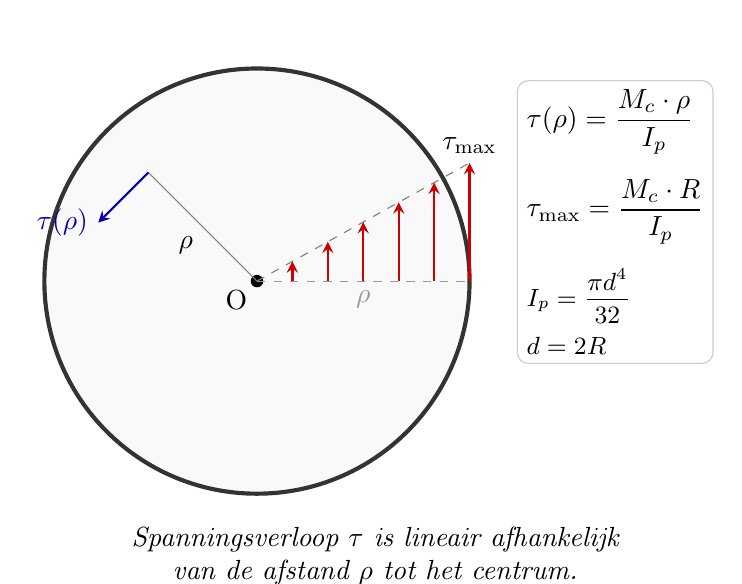
\begin{tikzpicture}[
			scale=1.5,
			>=stealth,
			% Styles
			shaft/.style={line width=1.5pt, draw=black!80},
			stress/.style={->, red!80!black, thick},
			profileLine/.style={dashed, gray, thin},
			dim/.style={<->, gray, thin}
		]

		% --- 1. DE AS (DOORSNEDE) ---
		\def\R{1.8}
		\draw[shaft, fill=gray!5] (0,0) circle (\R);
		\fill (0,0) circle (1.5pt) node[below left] {O};

		% --- 2. DE LINEAIRE SPANNINGSVERDELING (PROFIEL) ---
		% We tekenen de verdeling langs een horizontale as voor maximale duidelijkheid
		\draw[dashed, black!40] (0,0) -- (\R,0) node[midway, below] {$\rho$};

		% De "envelop" van de spanning (de schuine lijn die de lineaire groei toont)
		\draw[profileLine] (0,0) -- (\R, 1.0);

		% Reeks pijlen die de lineaire groei van tau tonen
		\foreach \x in {0.3, 0.6, 0.9, 1.2, 1.5, 1.8} {
				% Bereken de lengte van de pijl (lineair: lengte = constante * x)
				\pgfmathsetmacro{\len}{\x * (1.0 / \R)}
				\draw[stress] (\x, 0) -- (\x, \len);
			}

		% Label voor de maximale spanning aan de rand
		\node[anchor=south] at (\R, 1.0) {$\tau_{\text{max}}$};

		% --- 3. REPRESENTATIEVE PUNTEN (WILLEKEURIGE RADIUS) ---
		% Om aan te tonen dat het overal geldt, voegen we één willekeurige straal toe
		\def\ang{135}
		\def\rhoVal{1.3}
		\draw[gray, thin] (0,0) -- (\ang:\rhoVal) node[midway, below left, black] {$\rho$};
		\draw[stress, blue!70!black] (\ang:\rhoVal) -- ++(\ang+90:0.6) node[pos=1, left] {$\tau(\rho)$};

		% --- 4. FORMULES IN EEN NET KADER ---
		\node[draw=black!20, fill=white, rounded corners, anchor=west, align=left] at (2.2, 0.5) {
			$\tau(\rho) = \dfrac{M_c \cdot \rho}{I_p}$ \\[8pt]
			$\tau_{\text{max}} = \dfrac{M_c \cdot R}{I_p}$ \\[8pt]
			\small $I_p = \dfrac{\pi d^4}{32}$ \\[4pt]
			\small $d = 2R$
		};

		% --- 5. ONDERSCHRIFT ---
		\node[below=3cm, align=center, font=\itshape] at (1,0) {
			Spanningsverloop $\tau$ is lineair afhankelijk \\ van de afstand $\rho$ tot het centrum.
		};

	\end{tikzpicture}
	\caption{Torsiediagram: schuifspanning $\tau$ neemt lineair toe met de straal $\rho$; relevante formule staat buiten de doorsnede.}
	\label{fig:torsie_cirkel}
\end{figure}
Met het traagheidsmoment berekent als volgt (zie statica):
\newline
\theoriebox{\textbf{Polair traagheidsmoment voor een cirkelvormige doorsnede:} $I_p = \frac{\pi d^4}{32}$}

De combinatie van deze formules:

\frm{Maximale schuifspanning bij Draaien}{M_d = C_b \cdot d^{x_w}}{waarbij $M_d$ de maximaal toelaatbare schuifspanning is [\si{N.mm}], $C_b$ de schuifspanningcoëfficiënt [\si{N/mm^2}], $d$ de diameter [\si{mm}] en $x_w$ de schuifspanningsexponent [-].}


\frm{Maximale verspanningsmoment}{M_c = a\cdot M_b}{waarbij $M_c$ het verspaningsmoment is [\si{N.mm}], $a$ een factor [-] en $M_b$ het maximale verspanningsmoment [\si{N.mm}].}


Samen met het verspanningsmoment:

\medskip
\noindent\textbf{Afleiding van de maximale voeding $f_{\max}$ (twee methodes)}

\paragraph{1) Via het schuifspanningscriterium}
De maximale schuifspanning in de buitenvezel van een ronde doorsnede is
\[
	\tau_{\max}=\dfrac{16\,M_c}{\pi\,d^3}.
\]
Eis \(\tau_{\max}\le\tau_{\mathrm{allow}}\):
\[
	M_c \le \dfrac{\tau_{\mathrm{allow}}\,\pi\,d^3}{16}.
\]
Met \(M_c = C_m\,d^{x_M}\,f^{y_M}\) volgt
\[
	f_{\max} = \left(\dfrac{\tau_{\mathrm{allow}}\,\pi}{16\,C_m}\right)^{1/y_M} d^{(3-x_M)/y_M}.
\]

\paragraph{2) Via een momentlimiet}
Als \(M_c\le M_d=C_b\,d^{x_w}\) dan volgt
\[
	f_{\max} = \left(\dfrac{C_b}{C_m}\right)^{1/y_M} d^{(x_w-x_M)/y_M}.
\]

\paragraph{Speciale geval -- lineair}\hfill\\
Wanneer \(y_M=1\) en \(x_w-x_M=1\) volgt
\[
	f_{\max} = \dfrac{C_b}{C_m}\; d,
\]
wat overeenkomt met de eenvoudige vorm \(f_{\max}=C\cdot d\).




\frm{Maximale voeding bij boren}{f_{max} = C \cdot d}{waarbij $C$ een constante is [-], $d$ de diameter [\si{mm}] en $f_{max}$ de maximale voeding [\si{mm/omw}].}


\frm{Kracht $F_f$ is de kracht recht naar boven bij een boormachine}{F_f = C_f \cdot d^{X_f} \cdot f^{y_f}}{waarbij $F_f$ de voedingskracht is [\si{N}], $C_f$ de voedingskrachtcoëfficiënt [\si{N/mm^2}], $d$ de diameter [\si{mm}], $f$ de voeding [\si{mm/omw}] en $X_f, y_f$ de voedingskrachtsexponenten [-].}

Deze kracht zal een moment creeëren op de machine die hem kan buigen.
Dit is vooral bij C vormige structuren.

\begin{figure}[H]
	\centering
	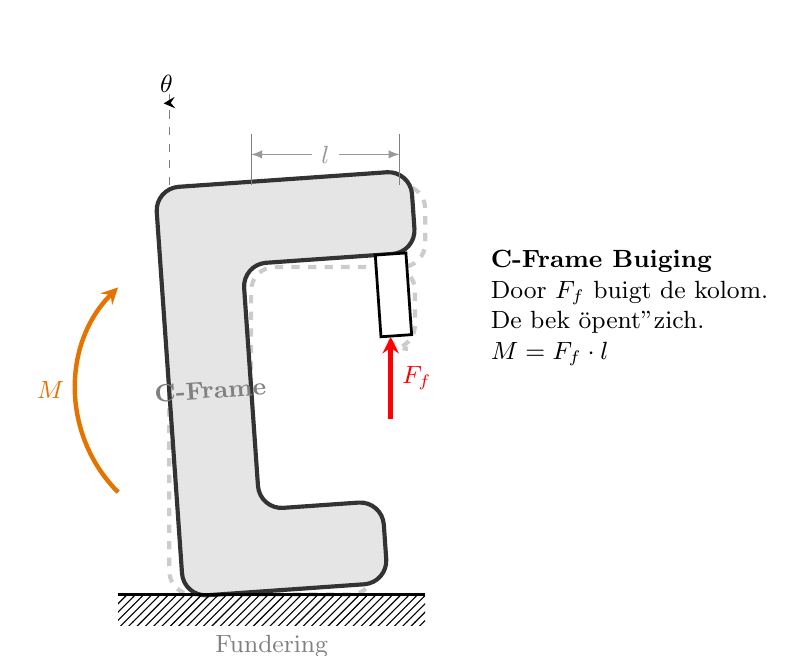
\begin{tikzpicture}[
			scale=1.3,
			>=stealth,
			every node/.style={font=\small},
			% Stijlen
			machine/.style={fill=gray!20, draw=black!80, line width=1.5pt, rounded corners=3mm},
			phantom/.style={draw=gray!40, line width=1.5pt, dashed, rounded corners=3mm},
			force/.style={->, ultra thick, red},
			dim/.style={<->, thin, gray!80, >=latex},
			ground/.style={fill, pattern=north east lines, draw=none}
		]

		% --- Parameters ---
		\def\bedL{2.0}      % Lengte onderbed
		\def\colW{0.8}      % Breedte kolom
		\def\colH{4.0}      % Hoogte kolom
		\def\armL{2.5}      % Lengte bovenarm (incl kolombreedte)
		\def\armThick{0.8}  % Dikte arm/bed
		\def\rotAngle{4}    % Rotatiehoek voor deformatie

		% --- Coördinaten ---
		\coordinate (BaseBL) at (0,0); % Linksonder

		% --- 1. GHOST (Oorspronkelijke staat) ---
		% We tekenen de outline van de C-vorm in dashed grijs
		% Vorm: L-shape onder + kolom + arm boven
		\draw[phantom]
		(0,0) -- (\bedL, 0) -- (\bedL, \armThick) -- (\colW, \armThick)
		-- (\colW, \colH-\armThick) -- (\armL, \colH-\armThick)
		-- (\armL, \colH) -- (0, \colH) -- cycle;

		% Spindel ghost
		\coordinate (SpindleTopGhost) at (\armL - 0.4, \colH-\armThick);
		\draw[phantom, fill=none] (SpindleTopGhost) rectangle ++(0.3, -0.8);

		% --- 2. DEFORMATIE (Vervormde staat) ---
		% Rotatiepunt: ergens in de "oksel" van de C
		\coordinate (Pivot) at (\colW/2, \colH/2);

		\begin{scope}[rotate around={\rotAngle:(Pivot)}]
			% De "open gebogen" machine
			% We simuleren de buiging door het hele bovenstuk iets te kantelen t.o.v. onderstuk? 
			% Nee, bij C-frame buigt de 'rug' (kolom) naar achteren en de bek gaat open.
			% Eenvoudige benadering: roteer de hele C-vorm om een punt laag in de rug.

			\draw[machine]
			(0,0) -- (\bedL, 0) -- (\bedL, \armThick) -- (\colW, \armThick)
			-- (\colW, \colH-\armThick) -- (\armL, \colH-\armThick)
			-- (\armL, \colH) -- (0, \colH) -- cycle;

			% Spindel (Vast aan arm)
			\coordinate (SpindleTop) at (\armL - 0.4, \colH-\armThick);
			\draw[fill=white, draw=black, line width=1pt] (SpindleTop) rectangle ++(0.3, -0.8) coordinate (SpindleTip);
			\node[below, xshift=2mm] at (SpindleTip) {}; % dummy

			% Annotatie op frame
			\node at (\colW/2, \colH/2) [rotate=\rotAngle, text=gray] {\textbf{C-Frame}};
		\end{scope}

		% --- 3. FUNDERING ---
		\draw[ground] (-0.5,-0.3) rectangle (\bedL+0.5, 0);
		\draw[thick] (-0.5,0) -- (\bedL+0.5, 0);
		\node[below, text=gray] at (\bedL/2, -0.3) {Fundering};

		% --- 4. KRACHTEN & MOMENT ---
		% F_f duwt de arm en bed uit elkaar. Hier tekenen we F_f op de spindel (werkstuk duwt terug)
		% De positie is nu geroteerd.
		% We nemen het midden van de onderkant van de spindel rect.
		\coordinate (ForcePos) at ($ (SpindleTop) + (0.15, -0.8) $);
		\draw[force] ($(ForcePos) + (0, -0.8)$) -- (ForcePos) node[midway, right] {$F_f$};

		% Moment M: Buigend moment in de rug
		% Pijl die "open buigen" aangeeft
		\draw[->, ultra thick, orange!90!black] (-0.5, \colH/2 - 1) to[bend left=45] node[left] {$M$} (-0.5, \colH/2 + 1);

		% --- 5. AFMETINGEN & LABELS ---
		% Hoek theta (overdreven weergegeven)
		% Vergelijking verticale lijn
		\draw[dashed, gray] (0, \colH) -- (0, \colH + 1.0);
		\draw[->, thick] (0, \colH + 0.8) arc (90:{90+\rotAngle}:0.8) node[midway, above] {$\theta$};

		% Arm lengte l (keel diepte)
		% Vanaf binnenkant kolom tot spindel as
		\draw[dim] (\colW, \colH + 0.3) -- (\armL - 0.25, \colH + 0.3) node[midway, fill=white] {$l$};
		\draw[gray, thin] (\colW, \colH) -- (\colW, \colH + 0.5);
		\draw[gray, thin] (\armL - 0.25, \colH) -- (\armL - 0.25, \colH + 0.5);

		% --- 6. TEKSTVAK ---
		\node[align=left, anchor=north west, fill=white, inner sep=5pt, rounded corners] at (3.0, 3.5) {
			\textbf{C-Frame Buiging}\\
			Door $F_f$ buigt de kolom.\\
			De bek "opent" zich.\\
			\small $M = F_f \cdot l$
		};

	\end{tikzpicture}
	\caption{C\nobreak\-vormig frame: axiale voedingskracht $F_f$ op het werkstuk (pivot) veroorzaakt een lichte kanteling (\(\theta\)) rond het werkstuk; de gestippelde lijn toont de gedraaide positie van het frame.}
	\label{fig:Cframe_moment}
\end{figure}


\FloatBarrier


\section{Boormachines en booroperaties in de industrie.}
\subsection{NC-gestuurde boormachines}
NC-gestuurde boormachines (Numerical Control) zijn computergestuurde machines die worden gebruikt voor het boren van gaten in materialen met
hoge precisie en herhaalbaarheid.
Deze machines maken gebruik van vooraf geprogrammeerde instructies
om de bewegingen van de boor en het werkstuk te regelen.
\newline

\subsection{Boren}
Hier zijn nog relevante type boren en hun toepassingen:
\begin{itemize}
	\item \textbf{Toepassingen:} verspanen van gaten voor bevestigingsmiddelen, passingen en nabewerkingen (ruimen, kotteren); wordt ook gebruikt als pilot voor grotere bewerkingen.
	\item \textbf{Belangrijke parameters:} snijsnelheid $v_c$, voeding $f$, snedediepte $a$, koelmiddel en spanenvorm.
	\item \textbf{Veelvoorkomende borentypes:}
	      \begin{itemize}
		      \item \textbf{Centerboor / positioneerboor:} korte, stijve boor om een startpunt te maken (voorkomt uitlopen van de boor).
		      \item \textbf{Steekboor (jobber / stub):} standaard boor voor algemene gaten; lengte en spiraaltype kiezen afhankelijk van diepte en spanenafvoer.
		      \item \textbf{Verzinkingsboor (countersink):} maakt een conische uitsparing voor schroefkoppen of voor ontbraamwerk.
		      \item \textbf{Split‑point / conische punt boren:} verbetert centrering en vermindert wander bij start.
	      \end{itemize}
\end{itemize}
\begin{figure}[ht]
	\centering
	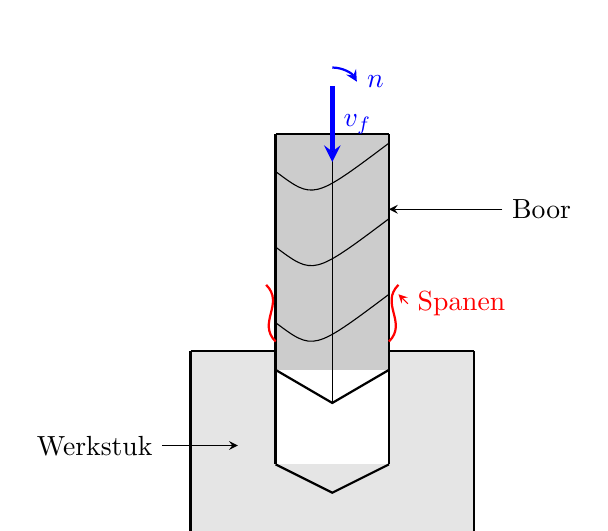
\begin{tikzpicture}[scale=1.2, >=stealth]
		% Werkstuk (doorsnede)
		\fill[gray!20] (-1.5, 0) rectangle (1.5, -2);
		\draw[thick] (-1.5, 0) -- (-0.6, 0);
		\draw[thick] (0.6, 0) -- (1.5, 0);
		\draw[thick] (-1.5, -2) -- (1.5, -2);
		\draw[thick] (-1.5, 0) -- (-1.5, -2);
		\draw[thick] (1.5, 0) -- (1.5, -2);

		% Gat
		\fill[white] (-0.6, 0) rectangle (0.6, -1.2);
		\draw[thick] (-0.6, 0) -- (-0.6, -1.2);
		\draw[thick] (0.6, 0) -- (0.6, -1.2);
		% Conische bodem van het gat
		\draw[thick] (-0.6, -1.2) -- (0, -1.5) -- (0.6, -1.2);

		% Boor (Twist Drill)
		\begin{scope}[yshift=-0.2cm]
			\def\drillW{1.2}
			\def\drillH{2.5}
			% Schacht
			\fill[gray!40] (-\drillW/2, 0) rectangle (\drillW/2, \drillH);
			\draw[thick] (-\drillW/2, 0) -- (-\drillW/2, \drillH);
			\draw[thick] (\drillW/2, 0) -- (\drillW/2, \drillH);
			\draw[thick] (-\drillW/2, \drillH) -- (\drillW/2, \drillH); % Top

			% Punt (118 graden punt)
			\draw[thick] (-\drillW/2, 0) -- (0, -0.35) -- (\drillW/2, 0);
			\draw[thin] (0, -0.35) -- (0, \drillH); % Aslijn

			% Spiralen (schematisch)
			\draw[thin] (-\drillW/2, 0.5) .. controls (-0.2, 0.2) .. (\drillW/2, 0.8);
			\draw[thin] (-\drillW/2, 1.3) .. controls (-0.2, 1.0) .. (\drillW/2, 1.6);
			\draw[thin] (-\drillW/2, 2.1) .. controls (-0.2, 1.8) .. (\drillW/2, 2.4);
		\end{scope}

		% Spanen (Chips)
		\draw[thick, red] (-0.6, 0.1) .. controls (-0.8, 0.3) and (-0.5, 0.5) .. (-0.7, 0.7);
		\draw[thick, red] (0.6, 0.1) .. controls (0.8, 0.3) and (0.5, 0.5) .. (0.7, 0.7);

		% Annotaties
		\draw[->] (1.8, 1.5) node[right] {Boor} -- (0.6, 1.5);
		\draw[->] (-1.8, -1.0) node[left] {Werkstuk} -- (-1.0, -1.0);
		\draw[->, red] (0.8, 0.5) node[right] {Spanen} -- (0.7, 0.6);

		% Beweging
		\draw[->, ultra thick, blue] (0, 2.8) -- (0, 2.0) node[midway, right] {$v_f$};
		\draw[->, thick, blue] (0, 3.0) arc (90:30:0.3) node[right] {$n$};

	\end{tikzpicture}
	\caption{Schematische weergave van een boorproces: een spiraalboor dringt het materiaal binnen, vormt een gat en voert spanen af.}
\end{figure}
\paragraph{Type boren}
\begin{itemize}
	\item \textbf{Verzinkingsboor}: Wordt gebruikt om een conische uitsparing te maken aan het begin van een gat, zodat schroefkoppen gelijk met het
	      oppervlak kunnen liggen.
	\item \textbf{Centerboor}: Wordt gebruikt om een startpunt te creëren.
	\item \textbf{Steekboor}: Wordt gebruikt voor het boren van algemene gaten.
\end{itemize}

\begin{figure}[ht]
	\centering
	\includegraphics[width=0.8\textwidth]{image44.png}
	\caption{Verschillende soorten boren}
\end{figure}

\subsection{Kotteren}
Als je een groot gat hebt en je kunt niet met een boor zo'n groot gat maken, dan kun je kotteren gebruiken.
Je kunt ook eventueel frezen maar dat zie je in het volgende hoofdstuk \ref{chap:Verspanen_Frezen}
Bij kotteren ga je de boor ook nog laten draaien waardoor je een groter oppervlak gaat verspanen.

\subsection{Draadtappen}
Draadtappen is het snijden van interne schroefdraad in een voorgeboord gat.

\begin{table}[ht]
	\centering
	\begin{tabularx}{0.8\textwidth}{|l|X|X|}
		\hline
		\textbf{Schroefdraad} & \textbf{Pitch (mm)} & \textbf{Tap‑boring (mm)} \\
		\hline
		M5~$\times$~0.8       & 0.8                 & 4.2                      \\
		\hline
		M6~$\times$~1.0       & 1.0                 & 5.0                      \\
		\hline
		M8~$\times$~1.25      & 1.25                & 6.75                     \\
		\hline
		M10~$\times$~1.5      & 1.5                 & 8.5                      \\
		\hline
	\end{tabularx}
	\caption{Veelvoorkomende metrische tap‑boringen}
\end{table}
\subsection{Ruimen}
Ruimen is een afwerkingsbewerking om een bestaand gat op nauwkeurige maat en met goede oppervlaktekwaliteit te brengen
Het zorgt ervoor dat je heel precies gaten kunt maken met een goede oppervlaktekwaliteit.
\begin{figure}[ht]
	\centering
	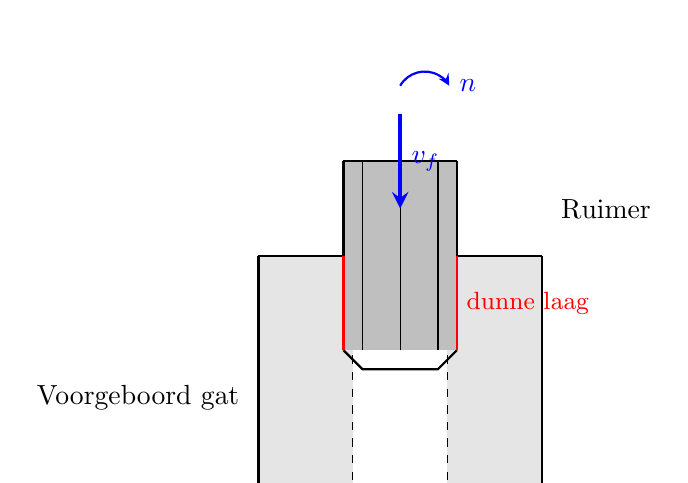
\begin{tikzpicture}[scale=1.2, >=stealth]
		% Werkstuk
		\fill[gray!20] (-1.5, 0) rectangle (1.5, -2.5);
		\draw[thick] (-1.5, 0) -- (1.5, 0);
		\draw[thick] (-1.5, -2.5) -- (1.5, -2.5);
		\draw[thick] (-1.5, 0) -- (-1.5, -2.5);
		\draw[thick] (1.5, 0) -- (1.5, -2.5);

		% Voorgeboord gat (iets kleiner dan de ruimer)
		\def\holeW{1.0}
		\fill[white] (-\holeW/2, 0) rectangle (\holeW/2, -2.5);
		\draw[dashed] (-\holeW/2, 0) -- (-\holeW/2, -2.5);
		\draw[dashed] (\holeW/2, 0) -- (\holeW/2, -2.5);

		% Ruimer (Reamer)
		\def\reamerW{1.2} % Iets breder dan het gat -> neemt materiaal af
		\def\reamerH{2.0}
		\begin{scope}[yshift=-1.0cm]
			\fill[gray!50] (-\reamerW/2, 0) rectangle (\reamerW/2, \reamerH);
			\draw[thick] (-\reamerW/2, 0) -- (-\reamerW/2, \reamerH);
			\draw[thick] (\reamerW/2, 0) -- (\reamerW/2, \reamerH);
			\draw[thick] (-\reamerW/2, \reamerH) -- (\reamerW/2, \reamerH);

			% Rechte tanden (Straight flutes)
			\draw[thin] (-0.4, 0) -- (-0.4, \reamerH);
			\draw[thin] (0, 0) -- (0, \reamerH);
			\draw[thin] (0.4, 0) -- (0.4, \reamerH);

			% Afgeschuinde onderkant (Chamfer)
			\draw[thick] (-\reamerW/2, 0) -- (-\reamerW/2 + 0.2, -0.2) -- (\reamerW/2 - 0.2, -0.2) -- (\reamerW/2, 0);
		\end{scope}

		% Materiaalafname indicatie
		\draw[red, thick] (-\reamerW/2, -1.0) -- (-\reamerW/2, 0);
		\draw[red, thick] (\reamerW/2, -1.0) -- (\reamerW/2, 0);
		\node[red, right] at (\reamerW/2, -0.5) {\small dunne laag};

		% Beweging
		\draw[->, ultra thick, blue] (0, 1.5) -- (0, 0.5) node[midway, right] {$v_f$};
		\draw[->, thick, blue] (0, 1.8) arc (150:30:0.3) node[right] {$n$};

		% Annotaties
		\node[right] at (1.6, 0.5) {Ruimer};
		\node[left] at (-1.6, -1.5) {Voorgeboord gat};

	\end{tikzpicture}
	\caption{Schematische weergave van ruimen: een ruimer verwijdert een dunne laag materiaal uit een voorgeboord gat voor hoge precisie en gladheid.}
\end{figure}


\begin{warningbox}[title=EXAMEN CHECKLIST: BOREN]
    \begin{itemize}
        \item \textbf{Nauwkeurigheid}: Ken de haalbare IT-klassen voor boren, kotteren en ruimen.
        \item \textbf{Krachten}: Begrijp dat bij boren de voedingskracht $F_f$ dominant is (axiale penetratie).
        \item \textbf{Torsie}: Leg uit hoe de maximale voeding $f_{max}$ wordt beperkt door de torsiesterkte van de boor.
        \item \textbf{Gereedschap}: Ken de types (twist drill, reamer, countersink) en hun functie.
        \item \textbf{C-Frame}: Begrijp het effect van de machinebuiging op de haaksheid van het gat.
    \end{itemize}
\end{warningbox}

\chapter{Verspanen: Frezen}
\label{chap:Verspanen_Frezen}

Frezen is een verspaningstechniek waarbij een roterend snijgereedschap, de frees, wordt gebruikt om materiaal van een werkstuk te verwijderen.
Het proces omvat het bewegen van de frees langs het oppervlak van het werkstuk om de gewenste vorm of maat te bereiken.

\textbf{- hoofdbeweging}
\newline
Je gereedschap de \textbf{frees} gaat roteren en het werkstuk kan ook roteren.
\newline
\textbf{- voedingsbeweging}
\newline
Het gereedschap of het werkstuk gaat bewegen om materiaal te verwijderen.
\newline

\subsection{Soorten frezen}
Als je gaat frezen via met de as-richting van de frees in de lengteas van de frees, noem je dit \textbf{mantelfrezen}.
\newline
Als je met de punt van de frees gaat frezen noem je dit \textbf{kopfrezen}.

\subsection{Geometrie van de frees}

Net zoals bij draaien en boren zijn er verschillende vlakken op de frees die verschillende functies hebben.
\begin{itemize}
	\item \textbf{Spaangroef}
	\item \textbf{Vrijloophoek}
	\item \textbf{Snijkant}
	\item \textbf{Snijvlak}
	\item \textbf{wighoek}
\end{itemize}

Deze hebben dezelfde eigenschappen als bij boren en draaien.
Je kunt meer info vinden bij Algemeen verspanen~\ref{chap:Algemeen verspanen}.

\begin{figure}[ht]
	\centering
	\includegraphics[width=0.6\textwidth]{image45.png}
	\caption{Geometrie van een mantelfrees}
\end{figure}


\section{krachtwerking bij frezen}

Net zoals bij draaien en boren zijn er verschillende krachten die op het werkstuk
en de frees werken tijdens het frezen.
Ze worden met de theorie van Kienzle berekend.

\begin{figure}[H]
	\centering
	\includegraphics[width=0.60\textwidth,trim=20 8 14 10,clip]{image46.png}
	\caption{Krachten op een frees}
	\label{fig:frees_krachten}
\end{figure}
\FloatBarrier

{\small
	De krachten op de frees zijn voornamelijk de snijkracht $F_c$ en de voedingskracht $F_f$; de terugdrukkracht $F_p$ is meestal kleiner en minder kritisch. Een goed begrip van deze krachten is essentieel voor het optimaliseren van snijparameters en het waarborgen van gereedschapslevensduur.
}
\begin{itemize}
	\item Snijkracht $F_c$: hoofdkracht die het snijproces aandrijft.
	\item Voedingskracht $F_f$: kracht die de voeding van de frees aandrijft.
	\item Terugdrukkracht $F_p$: kracht loodrecht op $F_c$ en $F_f$, meestal kleiner.
\end{itemize}

De snededikte is niet constant omdat je frees ronddraait. Voor berekeningen wordt de gemiddelde snededikte gebruikt.
\newline
\textbf{BELANGRIJK VOOR EXAMEN}\\
Je krachten op je frees zijn dus niet constant; zorg dat je dit weet voor het examen. Daarom nemen we het gemiddelde snededikte $h_{gem}$ zodat we toch een berekening hebben voor de kracht.

\theoriebox{\textbf{Gemiddelde snededikte bij Frezen:} $h_{gem} = f_z \cdot \sqrt{\dfrac{a}{d}}$\\\small}
\newline
waarbij $f_z$ de voeding per tand is, $a$ de snedediepte en $d$ de diameter van de frees.

\theoriebox{\textbf{Voeding per tand bij Frezen:} $f_z = \dfrac{f}{z_i}$\\\small}
\newline
waarbij $f$ de voeding is en $z_i$ het aantal tanden van de frees.

\theoriebox{\textbf{Snijsnelheid bij Frezen:} $v_c = \pi \cdot d \cdot n$\\\small}
\newline
waarbij $d$ de diameter van de frees is en $n$ het toerental.

\theoriebox{\textbf{Ingrijpingshoek bij Frezen:} $\displaystyle \phi = \arccos\!\left(1 - \dfrac{2a}{d}\right) \;\Rightarrow\; \cos\phi = 1 - \dfrac{2a}{d}$.\\\small}
\newline
waarbij $a$ de snedediepte is en $d$ de diameter van de frees.

\theoriebox{\textbf{Tanden per ingrijping}{$z_i = \frac{Q}{360}\cdot z$}}
\newline
waarbij $z_i$ het aantal tanden per ingrijping is,
$Q$ de ingrijpingshoek in graden en $z$ het totaal aantal tanden van de frees.
\newline

\frm{Snijkracht bij Frezen}{F_c = k_c \cdot b \cdot h_{gem}^{(1-e)} \cdot z_i}{waarbij $F_c$ de snijkracht is [\si{N}], $k_c$ de snijkrachtcoëfficiënt [\si{N/mm^2}], $b$ de snedebreedte [\si{mm}], $h_{gem}$ de gemiddelde snededikte [\si{mm}], $z_i$ het aantal tanden in de snede [-] en $e$ de snijkrachtexponent [-].}

\frm{Snijmoment bij Frezen}{M_c = C_m \cdot d^{x_M} \cdot f_z^{y_M} \cdot z_i}{waarbij $M_c$ het snijmoment is [\si{N.mm}], $C_m$ de momentcoëfficiënt [-], $d$ de diameter [\si{mm}], $f_z$ de voeding per tand [\si{mm/tand}], $z_i$ het aantal tanden in de snede [-] en $x_M, y_M$ de momentexponenten [-].}

\frm{Voedingskracht bij Frezen}{F_f = k_f \cdot b \cdot h_{gem}^{(1-e)} \cdot z_i}{waarbij $F_f$ de voedingskracht is [\si{N}], $k_f$ de voedingskrachtcoëfficiënt [\si{N/mm^2}], $b$ de snedebreedte [\si{mm}], $h_{gem}$ de gemiddelde snededikte [\si{mm}], $z_i$ het aantal tanden in de snede [-] en $e$ de voedingskrachtexponent [-].}

Bij frezen zijn de krachten op je frees niet constant.
De kracht op één tand per draaiing is parabolisch en als je de invloed van alle tanden samentelt krijg je een heuvelachtige
krachtcurve.
\begin{figure}[ht]
	\centering
	\includegraphics[width=0.5\textwidth]{47.png}
	\caption{Krachtcurve bij frezen}
\end{figure}

\section{Richting van frezen}
Er zijn twee richtingen van frezen:
\begin{itemize}
	\item \textbf{Meelopend frezen}: De frees draait in dezelfde richting als de voeding. Dit zorgt voor een betere oppervlaktekwaliteit en minder gereedschapsbelasting.
	\item \textbf{Tegenlopend frezen}: De frees draait in de tegenovergestelde richting van de voeding. Dit kan leiden tot een ruwer oppervlak en hogere gereedschapsbelasting.
\end{itemize}

\begin{figure}[ht]
	\centering
	\includegraphics[width=0.8\textwidth]{image48.png}
	\caption{Tegenlopend en meelopend frezen en de krachten die ze creëren}
	\label{fig:meelopend_tegenlopend}
\end{figure}

\begin{table}[ht]
	\centering
	\caption{Vergelijking: Tegenlopend vs Meelopend frezen}
	\label{tab:meelopend_vs_tegenlopend}
	\begin{tabularx}{\textwidth}{|l|X|X|}
		\hline
		\textbf{Kenmerk}      & \textbf{Tegenlopend}                               & \textbf{Meelopend}                                    \\
		\hline
		\textbf{Aandrijving}  & $F_h$ drukt werkstuk weg van frees.                & $F_h$ trekt werkstuk naar frees toe.                  \\
		\hline
		\textbf{Speling}      & Geen compensatie nodig; veiliger bij backlash.     & Spelingcompensatie onmisbaar.                         \\
		\hline
		\textbf{Spaanvorming} & Dun $\rightarrow$ dik (chip groeit tijdens snede). & Dik $\rightarrow$ dun (chip neemt af richting einde). \\
		\hline
		\textbf{Snijkracht}   & Stijgt geleidelijk tijdens ingreep.                & Stijgt sneller; hogere piekbelasting.                 \\
		\hline
		\textbf{Snijgedrag}   & Eerst wrijving, later snijden (meer smearing).     & Meteen snijden (scherpere insnijding).                \\
		\hline
		\textbf{Oppervlakte}  & Meestal matig.                                     & Meestal beter (glad).                                 \\
		\hline
		\textbf{Stabiliteit}  & Neiging tot klapperen / chatter.                   & Werkstuk wordt 'in klem' getrokken.                   \\
		\hline
		\textbf{Precisie}     & Minder voorspelbaar.                               & Kan preciezer zijn.                                   \\
		\hline
	\end{tabularx}
\end{table}
\FloatBarrier

\subsection{Wanneer kiezen: meelopend vs tegenlopend}
\textbf{Praktische richtlijnen:}
\begin{itemize}
	\item \textbf{Meelopend (climb milling)} -- kies dit bij een stijve machine en goede opspanning, vooral voor afwerking. De chipdikte neemt af tijdens de ingreep (dik $\rightarrow$ dun), er is minder wrijving bij de instap en doorgaans een betere oppervlaktekwaliteit en langere gereedschapslevensduur; vereist minimale backlash in de aandrijving.
	\item \textbf{Tegenlopend (conventional milling)} -- kies dit bij oudere of minder stijve machines, bij ruwe bewerkingen of wanneer er speling is. De chipdikte neemt toe tijdens de ingreep (dun $\rightarrow$ dik); bij de instap is er meer wrijving en kans op BUE, maar de methode is vaak veiliger voor onstabiele opstellingen of dunwandige onderdelen.
\end{itemize}

\paragraph{Effecten op oppervlakte en snedediepte}
\begin{itemize}
	\item \textbf{Oppervlaktekwaliteit:} Meelopend geeft doorgaans een gladdere afwerking; tegenlopend geeft meer wrijving bij instap en vaak een ruwere afwerking.
	\item \textbf{Snedediepte/productiviteit:} In een stijve opstelling maakt meelopend vaak hogere snededieptes en hogere voedingen mogelijk zonder kwaliteitsverlies; tegenlopend wordt vaak gebruikt voor grove, hoge‑volume snedes of wanneer de machine/opstelling de voorkeur geeft aan een voorzichtige instap.
\end{itemize}

\section{Soorten frezen}
\begin{itemize}
	\item \textbf{Mantelfrezen}: Hierbij wordt de zijkant van de frees gebruikt om materiaal te verwijderen. Dit is geschikt voor het maken van vlakke oppervlakken en contouren.
	\item \textbf{Kopfrezen}: Hierbij wordt de bovenkant van de frees gebruikt om materiaal te verwijderen. Dit is geschikt voor het maken van gaten, sleuven en andere complexe vormen.
	\item \textbf{Bolfrezen}: Hierbij wordt een frees met een bolvormige snijkant gebruikt, geschikt voor het maken van gebogen oppervlakken en complexe 3D-vormen.
	\item \textbf{Vormfrezen}: Hierbij wordt een frees met een specifieke vorm gebruikt om profielen en vormen in het materiaal te frezen.
	\item \textbf{Circulair frezen}: Hierbij wordt een cirkelvormige beweging gebruikt om gaten of cirkelvormige uitsparingen te maken.
	\item \textbf{Trekfrezen of Brootsen}: Hierbij wordt een speciaal gereedschap gebruikt om nauwkeurige vormen en profielen te maken door het materiaal te trekken.
\end{itemize}

\section{De Freesmachine}
Een freesmachine heeft een bank waar je werkstuk wordt op geklemd. Hierop steek je de mantel of kopfrees.
De frees gaat roteren en de bank gaat bewegen in de x,y en z-richting.


\begin{figure}[ht]
	\centering
	\includegraphics[width=0.8\textwidth]{image49.png}
	\caption{Weergave van een freesmachine}
\end{figure}

\begin{warningbox}[title=EXAMEN CHECKLIST: FREZEN]
    \begin{itemize}
        \item \textbf{Krachten}: Begrijp dat snijkrachten bij frezen variëren (heuvelachtig verloop) en dat we $h_{gem}$ gebruiken voor berekeningen.
        \item \textbf{Richting}: Ken het cruciale verschil tussen \keyterm{meelopend} (dik naar dun chip) en \keyterm{tegenlopend} (dun naar dik chip) frezen.
        \item \textbf{Geometrie}: Weet wat de ingrijpingshoek $\phi$ is en hoe die de belasting van de tanden bepaalt.
        \item \textbf{Technieken}: Onderscheid mantelfrezen (omtrek) en kopfrezen (kopse kant).
    \end{itemize}
\end{warningbox}

\chapter{Verspanen:Hybridetechnieken}

\section{Honen}

\begin{conceptbox}[title=Honen]
    Honen is een nabewerkingsproces voor cilindrische oppervlakken (zoals motorcilinders) om de nauwkeurigheid (IT3-IT5) en de oppervlaktekwaliteit te perfectioneren. Het kenmerkt zich door een roterende en axiaal oscillerende beweging, wat een karakteristiek kruislingse slijppatroon achterlaat.
\end{conceptbox}

Honen is een slijpoperatie met twee componenten en een heen een weergaande bewegingen.
\newline
\textbf{Hoofdbeweging}: Bij honen is de hoofdbeweging een roterende beweging.
\newline
\textbf{Voedingsbeweging}: Dit is de beweging waarmee het gereedschap of het
werkstuk langzaam wordt verplaatst om het slijpproces voort te zetten.
\newline
\textbf{Kasterpatronen}: Bij honen worden vaak specifieke kasterpatronen gebruikt om een gelijkmatige slijpoppervlakte te verkrijgen.
Honen helpt met het oppervalktekwaliteit tot en met (IT3)

\subsection{Lange-slag Honen}

\begin{figure}[ht]
	\centering
	\includegraphics[width=0.8\textwidth]{image56.png}
	\caption{Lange-slag honen}
	\label{fig:lange-slag-honen.png}
\end{figure}

Een hoonsteen wordt gebruikt om het oppervlakte van een cilinder te verbeteren.
De hoonsteen heeft een lange slag en beweegt heen en weer in de lengte van de cilinder.
Dit zorgt voor een betere oppervlaktekwaliteit en nauwkeurigheid van de cilinder.

Bij het honen ga je de toppen van de oppervalkteruwheid verwijderen.
Dit is anders bij het slijpen omdat die ook een licht oneven oppervlakte kan achterlaten.
\newline

% --- Illustratie: ruw oppervlak en resultaat na honen (scherpe toppen, geclipt) ---
\begin{figure}[ht]
	\centering
	\makebox[\textwidth][c]{%
		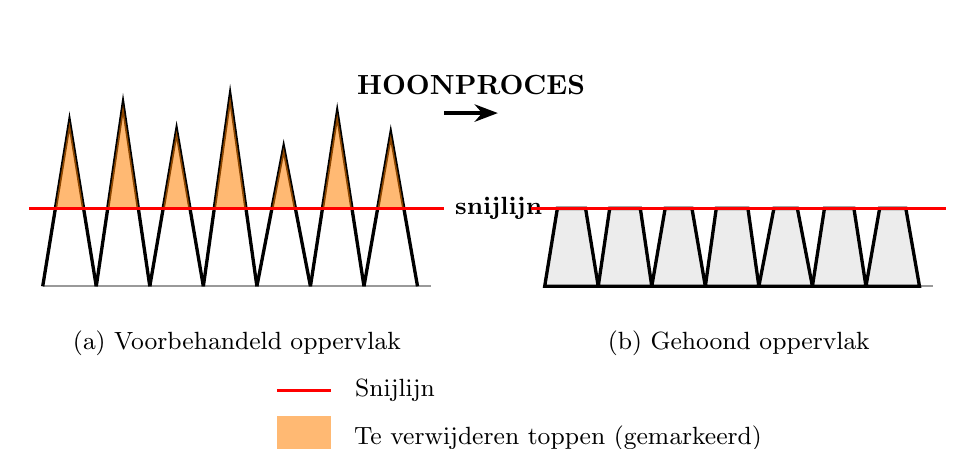
\begin{tikzpicture}[x=0.85cm, y=2.2cm, >=Stealth, every node/.style={font=\small}]
			% Parameters
			\def\L{5.8} % totale lengte
			\def\cut{0.45} % hoogte van de snijlijn (y-waarde)

			% --- (a) Voorbehandeld oppervlak ---
			\begin{scope}[shift={(0,0)}]
				% Basislijn
				\draw[black!40, thick] (0,0) -- (\L,0);

				% De toppen tekenen en de oranje delen inkleuren
				% Formaat: x-positie / hoogte
				\foreach \x/\h in {0.4/0.95, 1.2/1.05, 2.0/0.9, 2.8/1.1, 3.6/0.8, 4.4/1.0, 5.2/0.88} {
						% Teken de driehoek (contour)
						\draw[very thick, black] (\x-0.4, 0) -- (\x, \h) -- (\x+0.4, 0);

						% Bereken de snijpunten voor het oranje driehoekje (lineaire interpolatie)
						% x_breedte_op_snijlijn = 0.4 * (1 - cut/h)
						\pgfmathsetmacro{\xoffset}{0.4 * (1 - \cut/\h)}
						\fill[orange, opacity=0.55] (\x-\xoffset, \cut) -- (\x, \h) -- (\x+\xoffset, \cut) -- cycle;
					}

				% Snijlijn
				\draw[very thick, red] (-0.2, \cut) -- (\L+0.2, \cut) node[right, black]{\textbf{snijlijn}};

				% Label
				\node[below] at (\L/2, -0.2) {(a) Voorbehandeld oppervlak};
			\end{scope}

			% --- Hoonprocess pijl ---
			\draw[->, very thick] (6.0, 1.0) -- (6.8, 1.0);
			\node[above, font=\bfseries] at (6.4, 1.05) {HOONPROCES};

			% --- (b) Gehoond oppervlak (Trapezoïdes) ---
			\begin{scope}[shift={(7.5,0)}]
				\draw[black!40, thick] (0,0) -- (\L,0);

				\foreach \x/\h in {0.4/0.95, 1.2/1.05, 2.0/0.9, 2.8/1.1, 3.6/0.8, 4.4/1.0, 5.2/0.88} {
						% Bereken de breedte van de platte top op de snijlijn
						\pgfmathsetmacro{\xoffset}{0.4 * (1 - \cut/\h)}

						% Teken de trapezoïde (het restant onder de snijlijn)
						\draw[very thick, black, fill=gray!15]
						(\x-0.4, 0) -- (\x-\xoffset, \cut) -- (\x+\xoffset, \cut) -- (\x+0.4, 0) -- cycle;
					}

				% Snijlijn
				\draw[very thick, red] (-0.2, \cut) -- (\L+0.2, \cut);

				% Label
				\node[below] at (\L/2, -0.2) {(b) Gehoond oppervlak};
			\end{scope}

			% --- Legende ---
			\begin{scope}[shift={(3.5, -1.0)}]
				\draw[very thick, red] (0, 0.4) -- (0.8, 0.4) node[right=5pt, black] {Snijlijn};
				\fill[orange, opacity=0.55] (0, 0) rectangle (0.8, 0.25);
				\node[right=5pt] at (0.8, 0.125) {Te verwijderen toppen (gemarkeerd)};
			\end{scope}

		\end{tikzpicture}
	}

	\caption{(a) Voorbehandeld, ruw oppervlak met scherpe toppen; (b) resultaat na honen waarbij de bovenste delen van de toppen zijn verwijderd.}
	\label{fig:hoonprocess_schematic}
\end{figure}

\subsection{Korte-slag Honen}
Het enige verschil met lange-slag honen is de kinematica van het systeem.
Je werkstuk is opgespannen tussen twee tegenpunten die roteren.
Deze tegenpunten worden daan aangedreven met de hoonsteen op het oppervlakte.
Je gaat hier de hoonsteen op een cilindrisch oppervlakte toepassen zoals bij het nabewerkgen van zuigerstangen.
Je gaat sinusoïdale bewegingen maken met een korte slag.
De oppervlakte kwaliteit is enorm fijn.
\newline
\begin{figure}[ht]
	\centering
	\includegraphics[width=0.8\textwidth]{image57.png}
	\caption{Kortslag honen van een werkstuk}
	\label{fig:kortslag-honen.png}
\end{figure}

\section{Leppen}
Bij het leppen heb je enorm fijne korrels die in een paste, olie of gelei zitten.
De werstukken zitten in een cilinder of vat waarbij de stukken bewogen worden.

\subsection{Met vloeistof}
Het lepvloeistof beweegt tussen de stukken die het oppervlakte enorm fijn maken.
Tot en met \textbf{Ra = 0,1 µm, IT1} is mogelijk.

\textbf{Toepassingen}:
\newline
Bepaalde stukken hebben dit nodig zoals kogellagers of klepzittingen

\textit{Kijk zeker de video's op toledo om dit proces beter ge begrijpen}

\subsection{Finisheren met pasta}
Je drukt het werkstuk samen en pompt dan de gelei in het werkstuk om het oppervlakte te verbeteren.

\section{Geadvaseerde verspaningstechnieken en hybride technieken}

\subsection{hoge snelheid verspanen}
Bij hoge snelheid verspanen ga je enorm hoge snijsnelheden gebruiken in vergelijking met
conventionaleel verspanen.
\newline
\begin{figure}[ht]
	\centering
	\includegraphics[width=0.8\textwidth]{image58.png}
	\caption{Hoge snelheid verspanen in vergelijking met conventioneel verspanen}
	\label{fig:hoge_snelheid_verspanen.png}
\end{figure}

Deze spindles gaan tot 20,000 tot 30,000 RPM afhankelijk van het materiaal dat
je verspaand.

\subsection*{Extra}
Herinner je bij algemeen verspanen~\ref{chap:Algemeen verspanen} dat bij heel hoge
snijsnelheden je een \textbf{Softening effect} had die het makkelijker maakte om te verspanen.
Bij hoge snelheid verspanen zie je dit effect ook terugkomen. Alle warmte die ook gegenerateerd wordt gaan ook in
de spanen en gaan dus niet in het werkstuk defunderen en het oppervlakte aantasten.
\newline
\textbf{Toepassignen}
\newline
Je wilt enorm snel verspanningen doen.
Je moet dus je voeding $f$ en snijsnelheid $v_c$ enorm hoog zetten.
Deze techniek wordt vooral gebruikt bij aluminium en lichte metalen.
\newline
De tools zijn van hardmetaal gemaakt die ductiel genoeg zijn om de krachten te weerstaan.


\subsection{Hardverspanen}

\begin{conceptbox}[title=Hardverspanen]
    Hardverspanen is het direct draaien of frezen van geharde materialen ($>45$ HRC) die voorheen enkel geslepen konden worden. Dit vereist extreem stijve machines en gereedschappen zoals PCBN (Polycrystalline Cubic Boron Nitride).
\end{conceptbox}

Hardverspanen is het verspanen van harde materialen zoals gehard staal, keramiek en andere harde legeringen.
De ontwikkeling van hoge snelheidsfrezen en veel stevigere machines maakte dit mogelijk.
\newline
Je moet een negatieve spaanhoek gebruiken die meer kracht vraagt omdat de
afschuifhoek kleiner wordt. Als compensatie gebruik je kleine snededieptes om de krachten te beperken.
\newline
Nieuwe harde beitels en stevige machines die de hevige drukken aankan zorgt ervoor dat
hardverspanen niet eeuwig duurt.

\section{Hybrideprocessen}
hybride processen is een ruim domein waarbij je verschillende technieken toepast om
werkstukken te verspanen.
Je gaat dus twee technieken toepassen om bijvoorbeeld dingen makkelijker te verspanen
of om betere oppervlaktekwaliteit te krijgen.
\newline
Dit zijn vooral experimentele technieken die nog in ontwikkeling zijn.

\subsection {Laserondersteuning bij verspanen}
Je warmt het materiaal op met een laser. Het oppervlakte wordt warmer
en dus makkelijker om te verspanen.
\newline
Het is energie efficient omdat het warmere materiaal minder kracht kost om te verspanen.

\begin{figure}[ht]
	\centering
	\includegraphics[width=0.8\textwidth]{image59.png}
	\caption{Laserondersteuning bij verspanen}
	\label{fig:laserondersteuning-bij-verspanen.png}
\end{figure}

Het bepaal materiaal dat je moet gebruiken moet licht absorberen. Je wilt geen of zo weinig mogelijk reflectie of transmissie.
\newline
frm{Wat er gebeurt met licht die schijnt op een materiaal}{1 = $A+R+T$}{waarbij $A$ = absorptie, $R$ = reflectie en $T$ = transmissie}

\subsection{Draadvonken en slijpen}
\textit{(je ziet meer over draadvonken in een ander hoofdstuk)}
Het vonkproces is een thermisch proces. Je gaat eerst een stukje thermisch wegnemen. Bij normaal draadvonken
blijft een stuk gesmoleten materiaal achter op het oppervlakte maar door het slijpen ga je dit stuk wegnemen.

\subsection{ECM (Electro Chemical Machining) en slijpen}
Bij ECM ga je materiaal wegnemen door elektrochemische reacties.
Je hebt een anode en kathode die in een elektrolyt zitten.
Dit chemisch proces laat een ruw oppervlakte achter en oxidelagen.
Door het slijpen ga je dit ruw oppervlakte verbeteren en die laag verwijderen.

\subsection{Combinatie van ECM en frezen}
Je gaat frezen combineren met ECM.
De chemische bewerkingen laten een oxidelaag achter die je met frezen gaat verwijderen.

\textit{(Deze technieken zijn niet super belangrijk om vanbuiten te kennen maar je moet zien dat je nadelen van een proces kunt oplossen met een ander proces)}

\begin{warningbox}[title=EXAMEN CHECKLIST: HYBRIDETECHNIEKEN]
    \begin{itemize}
        \item \textbf{Honen}: Weet dat dit dient voor het verwijderen van toppen in cilinders (IT3-IT5).
        \item \textbf{Leppen}: Begrijp dat dit werkt met vrije korrels in een pasta voor extreme gladheid (IT1).
        \item \textbf{Hoge Snelheid Verspanen (HSM)}: Leg uit waarom de warmte bij HSM grotendeels in de spaan gaat (Softening effect).
        \item \textbf{Hardverspanen}: Ken de noodzaak voor negatieve spaanhoeken en stijve machines.
        \item \textbf{Hybride Concept}: Begrijp hoe lasers of ECM kunnen helpen om krachten te verlagen of oppervlakken te finishen.
    \end{itemize}
\end{warningbox}

\chapter{Verspanen:Slijpen}

\begin{conceptbox}[title=Onbepaalde snijkant]
    In tegenstelling tot draaien of frezen, heeft slijpen geen vaste snijkantgeometrie. Het oppervlak van de slijpsteen bestaat uit ontelbare, willekeurig georiënteerde korrels die materiaal afnemen met een sterk negatieve spaanhoek.
\end{conceptbox}

Slijpen is een verspaningstechniek waarbij een roterend schijfvormig gereedschap,
de slijpschijf, wordt gebruikt om materiaal van een werkstuk te verwijderen.
Verspannen gebeurt door een slijpsteen die kleine deeltjes materiaal \textbf{Snijkorrels} van het werkstuk afneemt.
Dit oppervlakte is onbepaald en dus is de geometrie niet gekent.
\newline
De snijkorrels kunnen oftewel vrij liggen of gebonden zijn in een matrix.
\newline
\textbf{Vrije snijkorrels:} losse korrels die losjes op het werkstuk inwerken of in suspensie of pasta. Voorbeelden:
\begin{itemize}
	\item \textbf{Leppen}: korrels in een pasta om zeer nauwkeurige oppervlakken te verkrijgen.
	\item \textbf{Stralen}: korrels in een straal om vuil of roest te verwijderen.
\end{itemize}
Je kunt dus korrels door het werkstuk sturen om het oppervlaktekwaliteit te verbeteren.
\newline
Korrel kunnen ook gebonden zijn in een matrix.
\newline
\textbf{Gebonden snijkorrels:} korrels die vastzitten in een matrixmateriaal. Voorbeelden:
\begin{itemize}
	\item \textbf{Slijpschijven}: korrels gebonden in een harde matrix voor het slijpen van metalen.
	\item \textbf{Schuurpapier}: korrels gebonden op papier of stof voor handmatig schuren.
	\item \textbf{Honen}: korrels gebonden in een zachte matrix voor het verbeteren van de oppervlakteafwerking en nauwkeurigheid van gaten.
\end{itemize}


\subsection{Frezen met onbepaalde snijkanten}
Bij slijpen heb je een grote negatieve \textbf{Spaanhoek} wat het moeilijker maakt om te verspanen.
De krachtwerking is dus veel hoger. Maar je \textbf{Snedediepte} is veel kleiner dus die combenseren elkaar.

Een slijpsteen kun je definieren als een frees met onbepaalde snijkanten.
\newline

\begin{figure}[ht]
	\centering
	\includegraphics[width=0.8\textwidth]{image50.png}
	\caption{Spaanvorming bij slijpen}
	\label{Spaanvorming bij slijpen}
\end{figure}

De korrel hier heeft een enorm negatieve spaanhoek. De spaanvorming is enorm klein maar omdat de korrels
zo klein en hard zijn kun je zelfs heel harde materialen slijpen.
\newline
\subsection{Eigenschappen van slijpen}
\begin{enumerate}
	\item \textbf{Snijsnelheid $v_c$}: De snelheid is ongeveer 25 tot 60 m/s, Heel hoge snelheden.
	\item \textbf{Krachten $F_c$}: De krachten zijn hoog door de negatieve spaanhoek en omdat je harde materialen kunt slijpen.
	\item \textbf{Warmteontwikkeling}: Veel energie gaat verloren als warmte, slijpen kan aan het oppervlakte een temperatuur van \textbf{800 tot 900°C} veroorzaken.
	      Dit kan leiden tot thermische beschadiging van het werkstuk. Je hebt dus materiaalveranderingen aan het oppervlakte.
	      Intensieve koeling is dus nodig.
	\item \textbf{Snedediepte $a$}: Zeer kleine snededieptes, typisch in de orde van micrometers.
	\item \textbf{Slijtage van de slijpkorrel}: Slijpkorrels worden bot en vallen er dan af.
	      Je moet de slijpschijf dus regelmatig vernieuwen of terug op maat brengen. Je neemt dan een stuk van het oppervlakte af.
	      Dit noemt(dressing).
	\item \textbf{Oppervlaktekwaliteit}: Slijpen kan zeer fijne oppervlakteafwerkingen bereiken, vaak in de orde van enkele micrometers $R_a$.
	\item \textbf{Nauwkeurigheid}: Slijpen gaat op machine die enorm stevig zijn en dus niet veel bewegen tijdens het slijpen.
	      Hierdoor kun je zeer nauwkeurige afmetingen bereiken.
	\item \textbf{Toepassingen}: Slijpen kan toegapast worden op zelfs zeer harde materialen zoals gehard staal, keramiek en zelfs diamant.
\end{enumerate}

\subsection{Parameters slijpsteen}

\begin{itemize}
	\item \textbf{Korrelgrootte}: Grotere korrels
	      verwijderen materiaal sneller maar geven een ruwere afwerking; kleinere korrels geven een fijnere afwerking.
	\item korrelgrote
	\item \textbf{Bindmiddel}: Het materiaal dat de korrels bij elkaar houdt, beïnvloedt de slijpsteen's hardheid en duurzaamheid.
	\item Hardheid van de slijpsteen: Hardere slijpstenen zijn duurzamer maar kunnen ook sneller de korrels verliezen.
	\item Structuur
\end{itemize}

\begin{figure}[ht]
	\centering
	\includegraphics[width=0.8\textwidth]{image51.png}
	\caption{Doorsnede van een slijpschijf}
	\label{fig:slijpsteen doorsnede.png}
\end{figure}
\subsubsection{Korrelmateriaal}
\textbf{Natuurlijke korrels} zijn kwarts, korundum en diamant.
\newline
\textbf{Kunstmatige korrels} zijn siliciumcarbide en aluminiumoxide.
\newline
\subsubsection{Korrelgroot}
De korrelgrootte bepaald hoeveel je kunt afnemen.
Grote korrels -> meer afnemen maar je oppervlaktekwaliteit is slechter.
Kleine korrels -> minder afnemen maar je oppervlaktekwaliteit is beter.
\newline
Korrelgrootte wordt aangegeven door mazen per $\text{inch}^2$.

\subsection{Hardheid van de slijpsteen}

\begin{conceptbox}[title=Slijpverhouding (G-ratio)]
    De slijpverhouding $G$ wordt gedefinieerd als het volume verwijderd materiaal gedeeld door het volume verloren slijpsteen. Een hoge $G$-waarde duidt op een efficiënt proces waarbij weinig gereedschapsslijtage optreedt.
    \[ G = \frac{V_{verwijderd}}{V_{steen}} \]
\end{conceptbox}

De hardheid is de sterkte van de korrels.
De slijpverhouding $G$ = $\frac{\text{volume verspaand materiaal}}{\text{volume slijpschijf per tijdseenheid}}$.
Een grote $G$ kan je veel materiaal afnemen tegenover hoeveel slijpschijf je verliest.
\newline
een kleine $G$ betekent dat je veel slijpschijf verliest tegenover hoeveel materiaal je afneemt.
\newline
Je kunt geen hard materiaal slijpen met een zachte slijpsteen omdat de korrels dan te snel bot worden.
\subsubsection{Bindmiddel}
Het bindmiddel houdt de korrels bij elkaar.
een paar voorbeelden zijn keramisch klei, mineralen, metaal en elastische materialen.
\newline
\theoriebox{Bijvoorbeeld bij pasta slijpen word een elastisch bindmiddel zodat de korrels overal op het werkstuk kunnen bewegen. We spreken dan niet van een slijpverhouding $G$ omdat die niet relevant is}

\subsubsection{Structuur}
De grote van de porien in verhouding tot het volumeaandeel bindmiddel en korrels.
\newline
Die porien zijn belangrijk. Die zijn kleine openingen tussen de korrels.
Stukjes spaan gaan in die porien. De poriegrootte moet je aanpassen afhankelijk van de operatie en het contacttijd van de slijpschijf op het werkstuk.
\newline

Met al deze dingen kunnne een slijpsteen karateriseren.

\textbf{WETEN DAT AL DEZE DIINGEN EEN SLIJPSTEEN KARATERISEREN}

\begin{figure}[ht]
	\centering
	\includegraphics[width=0.8\textwidth]{image52.png}
	\caption{}
	\label{fig:karateriseren van slijpsteen.png}
\end{figure}

\section{temperaturen bij slijpen}

$70{\%}$ van de energie die je inbrengt bij het slijpen gaat verloren als warmte.
dit kan leiden tot thermische beschadiging van het werkstuk.
Je moet oppassen voor
\begin{itemize}
	\item \textbf{Vonken}
	\item \textbf{Structuurveranderingen}
	\item \textbf{Verbranding}
	\item \textbf{Scheurtjes}
	\item \textbf{Residuële spanningen}
\end{itemize}

Je moet dus voldoende koelen of nog een laatste warmtebehandeling doen na het slijpen.
\begin{figure}[ht]
	\centering
	\includegraphics[width=0.6\textwidth]{image53.png}
	\caption{Warmte bij Slijpen}
	\label{fig:warmte_bij_slijpen.png}
\end{figure}

\section{Slijptechnieken}

\begin{figure}[ht]
	\centering
	\includegraphics[width=0.6\textwidth]{image54.png}
	\caption{Alle soorten slijptechnieken}
	\label{fig:Slijptechnieken.png}
\end{figure}

Profielslijpen is slijpen van een bepaald profiel. Je slijpsteen heeft dus een gewenste vorm,
waar je het werkstuk mee slijpt.
\newline

\textit{Tip, is hij niet veel op ingegaan.}


\section{De slijpmachine}
Slijpmachines zijn enorm stijve machines omdat je enorm
je snedediepte enorm klein is kan kleine bewegingen ervoor zorgen dat je ineens niet meer slijpt.
Je moet dus in orde van micrometer werken.

\subsection{Centerloos slijpen}
Centerloos slijpen is een slijptechniek waarbij het werkstuk niet wordt vastgehouden door een as of klem, maar in plaats daarvan wordt ondersteund door twee rollen en aangedreven door een derde rol.
\begin{figure}[ht]
	\centering
	\includegraphics[width=0.8\textwidth]{image55.png}
	\caption{Centerloos slijpen}
	\label{fig:centerloos_slijpen.png}
\end{figure}

\subsection{Profielslijpen}
Zoals hiervoor gezegd. Je slijpt een bepaald profiel met een slijpsteen die dat profiel heeft.

\begin{warningbox}[title=EXAMEN CHECKLIST: SLIJPEN]
    \begin{itemize}
        \item \textbf{Onbepaalde snijkant}: Begrijp het verschil met gedefinieerde snijkanten en de impact van de negatieve spaanhoek.
        \item \textbf{Karakterisering}: Ken de 5 factoren: korrelmateriaal, korrelgrootte, hardheid, bindmiddel en structuur (porositeit).
        \item \textbf{Warmte}: Weet dat $70\%$ van de energie in warmte gaat ($900^\circ$C) en ken de risico's (TAZ, scheuren).
        \item \textbf{Dressing}: Leg uit waarom een slijpsteen regelmatig "gedressed" moet worden (scherp maken en profileren).
        \item \textbf{Centerloos slijpen}: Begrijp het principe en de voordelen voor massaproductie.
    \end{itemize}
\end{warningbox}

\chapter{Fysische, Chemische afnemende bewerkingen}

\section{Vonkerosie}

\begin{conceptbox}[title=EDM (Electro Discharge Machining)]
    EDM verwijdert materiaal door gecontroleerde elektrische ontladingen (vonken) tussen een elektrode en het werkstuk in een isolerend diëlektricum. Het proces is thermisch: materiaal wordt lokaal gesmolten en verdampt zonder mechanische krachten.
\end{conceptbox}

\textbf{EDM (Electro Discharge Machining)} of \textbf{vonkerosie} is een \textbf{verspaningstechniek} waarbij materiaal wordt
verwijderd door middel van \textbf{elektrische vonken}.
Je hebt een \textbf{elektrode} en een \textbf{werkstuk} die in een \textbf{vloeistof} (die als \textbf{isolator} fungeert zoals bijvoorbeeld gedestilleerd water) zitten.
Wanneer er een \textbf{hoge spanning} wordt aangelegd tussen de elektrode en het werkstuk, ontstaat
een elektrische vonk die het materiaal op het werkstuk smelt en wegneemt.
\newline
Je kunt geen normaal water gebruiken omdat er mineralen in zitten die wel geleiden.

\begin{figure}[ht]
	\centering
	\includegraphics[width=0.5\textwidth]{image60.png}
	\caption{Vonkerosie proces}
	\label{fig:vonkerosie_proces.png}
\end{figure}

\begin{figure}[ht]
	\centering
	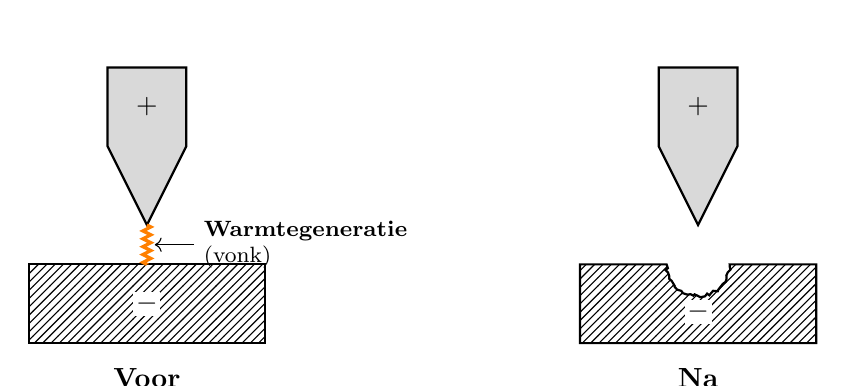
\begin{tikzpicture}
		\tikzset{
			elec/.style={fill=gray!30, draw=black, thick},
			work/.style={fill=gray!10, draw=black, thick, pattern=north east lines},
			spark/.style={decoration={zigzag, segment length=1mm, amplitude=0.5mm}, decorate, draw=orange, very thick},
			rough/.style={decorate, decoration={random steps, segment length=0.4mm, amplitude=0.2mm}}
		}

		% LEFT: BEFORE
		\begin{scope}[local bounding box=before]
			% Electrode (Top +)
			\draw[elec] (-0.5, 2.5) -- (-0.5, 1.5) -- (0, 0.5) -- (0.5, 1.5) -- (0.5, 2.5) -- cycle;
			\node at (0, 2) {$+$};

			% Workpiece (Bottom -)
			\draw[work] (-1.5, 0) rectangle (1.5, -1);
			\node[fill=white, inner sep=1pt] at (0, -0.5) {$-$};

			% Spark
			\draw[spark] (0, 0.5) -- (0, 0);
			% Text moved to the right with a pointer to the spark
			\node[right, font=\footnotesize, align=left] (lbl) at (0.6, 0.25) {\textbf{Warmtegeneratie}\\(vonk)};
			\draw[->, thin] (lbl.west) -- (0.1, 0.25);

			\node[below=0.2cm] at (0, -1) {\textbf{Voor}};
		\end{scope}

		% RIGHT: AFTER
		\begin{scope}[xshift=7cm, local bounding box=after]
			% Electrode (Top +)
			\draw[elec] (-0.5, 2.5) -- (-0.5, 1.5) -- (0, 0.5) -- (0.5, 1.5) -- (0.5, 2.5) -- cycle;
			\node at (0, 2) {$+$};

			% Workpiece (Bottom -) with ROUGH crater
			% Replaced smooth arc with a decorated path for roughness
			\draw[work] (-1.5, 0) -- (-0.4, 0)
			decorate[rough] { arc[start angle=180, end angle=360, radius=0.4] }
			-- (1.5, 0) -- (1.5, -1) -- (-1.5, -1) -- cycle;

			\node[fill=white, inner sep=1pt] at (0, -0.6) {$-$};

			\node[below=0.2cm] at (0, -1) {\textbf{Na}};
		\end{scope}

	\end{tikzpicture}
	\caption{Principe van vonkerosie: warmtegeneratie door elektrische ontlading zorgt voor materiaalafname (ruw oppervlak).}
	\label{fig:vonkerosie_principe}
\end{figure}

\subsection{Componenten van een EDM-systeem}
Bij een vonkerosie-opstelling (zoals in \cref{fig:vonkerosie_proces.png}) zijn de volgende componenten cruciaal:
\begin{itemize}
	\item \textbf{Pulsgenerator}: De energiebron die hoogfrequente DC-pulsen levert. Hij regelt de aan-tijd ($t_{on}$) en uit-tijd ($t_{off}$), wat de ruwheid en snelheid bepaalt.
	\item \textbf{Diëlektricum}: De isolerende vloeistof. Het zorgt voor isolatie tot de doorslagspanning wordt bereikt, koelt het proces en spoelt de deeltjes weg.
	\item \textbf{Pomp \& Filtersysteem}: De vloeistof wordt rondgepompt. Het filter is essentieel om de verwijderde metaaldeeltjes (swarf) uit het diëlektricum te halen. Vervuild diëlektricum leidt tot instabiele vonken of kortsluiting (arc-ing).
	\item \textbf{Servosysteem}: Handhaaft een constante, zeer kleine afstand (gap) tussen elektrode en werkstuk.
\end{itemize}

\begin{figure}[ht]
	\centering
	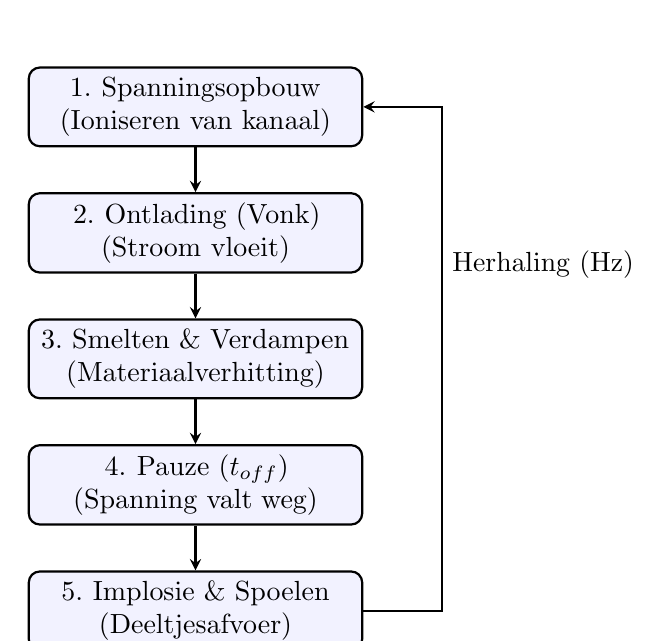
\begin{tikzpicture}[node distance=1.6cm, auto,
			procstep/.style={rectangle, draw=black, thick, fill=blue!5, text width=4cm, align=center, rounded corners, minimum height=1cm},
			arrow/.style={thick, ->, >=stealth}
		]
		\node (start) [procstep] {1. Spanningsopbouw \\ (Ioniseren van kanaal)};
		\node (spark) [procstep, below of=start] {2. Ontlading (Vonk) \\ (Stroom vloeit)};
		\node (heat)  [procstep, below of=spark] {3. Smelten \& Verdampen \\ (Materiaalverhitting)};
		\node (off)   [procstep, below of=heat] {4. Pauze ($t_{off}$) \\ (Spanning valt weg)};
		\node (flush) [procstep, below of=off] {5. Implosie \& Spoelen \\ (Deeltjesafvoer)};

		\draw [arrow] (start) -- (spark);
		\draw [arrow] (spark) -- (heat);
		\draw [arrow] (heat) -- (off);
		\draw [arrow] (off) -- (flush);
		\draw [arrow] (flush.east) -- ++(1,0) |- node[anchor=west, yshift=-2cm] {Herhaling (Hz)} (start.east);

	\end{tikzpicture}
	\caption{Cyclus van één EDM-puls: van spanningsopbouw tot spoelen.}
	\label{fig:edm_puls_flow}
\end{figure}

Je benedenplaat wordt \textbf{negatief geladen} en de elektrode \textbf{positief}.
Er is dan een puls van \textbf{discharge} die een stukje materiaal wegneemt.
\textbf{Pulsen} hebben een \textbf{frequentie} tussen de 100khz tot 1Mhz.
Je genereert dan veel discharges die opbouwen zodat je lijnen stap per stap kunt wegnemen.
\newline
De afstand tussen de elektrode en het werkstuk is enorm klein maar enorm belangrijk.
Moest de elektrode op het werkstuk komen, dan zou er een \textbf{kortsluiting} zijn.
\newline
De \textbf{spaanvorming} is bolvormig.
\newline
De pulsenergie wordt gegeven door de formule
\frm{Pulsenergie tijdens vonkfrezen}{W_e = \int_0^{t_e} U_e I_e \, dt}{waarbij $W_e$ de pulsenergie is [\si{J}], $U_e$ de doorslagspanning [\si{V}], $I_e$ de stroom [\si{A}] en $t_e$ de pulstijd [\si{s}].}
\begin{figure}[ht]
	\centering
	\includegraphics[width=0.45\textwidth]{image61.png}
	\includegraphics[width=0.45\textwidth]{image62.png}
	\caption{Stapsgewijs een puls en de bijbehorende spannings- en stroomcurves en tabel van alle parameters.}
	\label{fig:edm_elektrode_vormen.png}
\end{figure}

Het vonkproces verloopt in drie cyclische fases die zich duizenden keren per seconde herhalen:

\begin{figure}[ht]
	\centering
	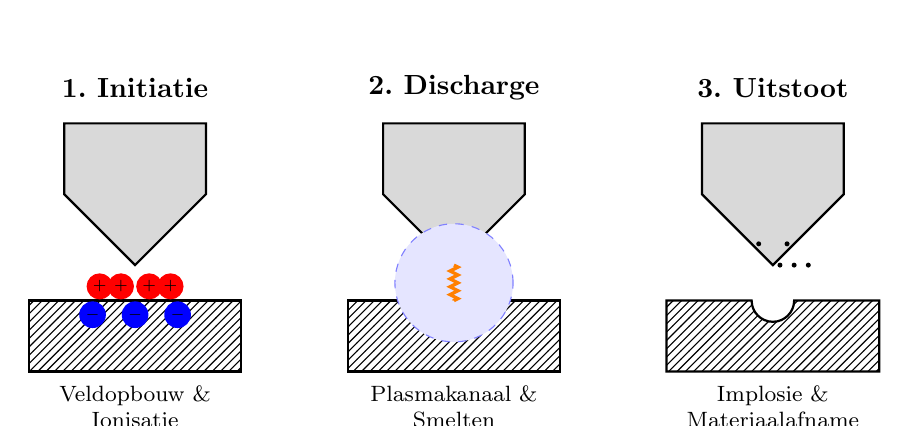
\begin{tikzpicture}[scale=0.9,
			elec/.style={fill=gray!30, draw=black, thick},
			work/.style={fill=gray!10, draw=black, thick, pattern=north east lines},
			gas/.style={circle, draw=blue!50, fill=blue!10, dashed, minimum size=1.5cm},
			spark/.style={decoration={zigzag, segment length=1mm, amplitude=0.5mm}, decorate, draw=orange, very thick}
		]
		% Phase 1: Initiation
		\begin{scope}[local bounding box=p1]
			\node at (0, 3) {\textbf{1. Initiatie}};
			\draw[elec] (-1, 2.5) -- (-1, 1.5) -- (0, 0.5) -- (1, 1.5) -- (1, 2.5) -- cycle;
			\draw[work] (-1.5, -1) rectangle (1.5, 0);

			% Ions
			\foreach \x in {-0.5, -0.2, 0.2, 0.5} \node[circle, fill=red, inner sep=1pt] at (\x, 0.2) {\tiny $+$};
			\foreach \x in {-0.6, 0, 0.6} \node[circle, fill=blue, inner sep=1pt] at (\x, -0.2) {\tiny $-$};
			\node[font=\footnotesize, align=center] at (0, -1.5) {Veldopbouw \& \\ Ionisatie};
		\end{scope}

		% Phase 2: Discharge
		\begin{scope}[xshift=4.5cm, local bounding box=p2]
			\node at (0, 3) {\textbf{2. Discharge}};
			\draw[elec] (-1, 2.5) -- (-1, 1.5) -- (0, 0.5) -- (1, 1.5) -- (1, 2.5) -- cycle;
			\draw[work] (-1.5, -1) rectangle (1.5, 0);

			% Gas bubble & Spark
			\node[gas] at (0, 0.25) {};
			\draw[spark] (0, 0.5) -- (0, 0);

			\node[font=\footnotesize, align=center] at (0, -1.5) {Plasmakanaal \& \\ Smelten};
		\end{scope}

		% Phase 3: Ejection
		\begin{scope}[xshift=9cm, local bounding box=p3]
			\node at (0, 3) {\textbf{3. Uitstoot}};
			\draw[elec] (-1, 2.5) -- (-1, 1.5) -- (0, 0.5) -- (1, 1.5) -- (1, 2.5) -- cycle;
			% Crater
			\draw[work] (-1.5, 0) -- (-0.3, 0) arc(180:360:0.3) -- (1.5, 0) -- (1.5, -1) -- (-1.5, -1) -- cycle;

			% Debris
			\foreach \r in {0.1, 0.3, 0.5} \fill[black] (\r, 0.5) circle (1pt);
			\foreach \r in {-0.2, 0.2} \fill[black] (\r, 0.8) circle (1pt);

			\node[font=\footnotesize, align=center] at (0, -1.5) {Implosie \& \\ Materiaalafname};
		\end{scope}
	\end{tikzpicture}
	\caption{De drie fases van een EDM-puls.}
	\label{fig:edm_phases}
\end{figure}

\begin{enumerate}
	\item \textbf{De initiatiefase (Ontsteking):}
	      Er wordt een spanning aangelegd tussen elektrode en werkstuk. Het elektrisch veld zorgt ervoor dat
	      vrije elektronen en ionen in het diëlektricum versnellen en botsen.
	      Dit creëert een \emph{sneeuwbaleffect} (lawine-ionisatie), waardoor er een geleidend ionisatiekanaal ontstaat.

	\item \textbf{De dischargefase (Ontlading):}
	      Zodra het kanaal geleidend is, volgt de hoofdontlading (de vonk).
	      De stroomsterkte piekt en er ontstaat een \textbf{gasbel} van plasma rondom de vonk.
	      De ionen botsen met hoge kinetische energie op het werkstuk, wat wordt omgezet in extreme hitte ($8000\text{--}12000\,^\circ\text{C}$).
	      Hierdoor smelt en verdampt een klein deel van het werkstuk (en in mindere mate de elektrode).

	\item \textbf{De uitstootfase (Implosie):}
	      De stroom wordt plotseling onderbroken (shutdown).
	      De temperatuur daalt en de gasbel implodeert krachtig.
	      Door deze implosie wordt het gesmolten materiaal uit de krater weggeschoten in het diëlektricum,
	      waar het stolt tot kleine bolletjes (swarf). Het diëlektricum spoelt de opening schoon voor de volgende puls.
\end{enumerate}

\begin{figure}[ht]
	\centering
	\includegraphics[width=0.6\textwidth]{image63.png}
	\caption{Een vonk in vergelijking met meerdere vonken}
	\label{fig:1vonkenmeerderevonken.png}
\end{figure}

\section{Performance van EDM}

De materiaal afnamen (material removal rate) gaat over quibice centermeter per minuut.
Deze materiaalafname is veel lager dan bij spanen.
\newline
Gereedsschap slijtage is ook een probleem bij EDM. Ratio
\frm{Gereedschapslijtage bij EDM}{\vartheta = \frac{\text{Volume gereedschap versleten}}{\text{Volume werkstuk verspaand}}}{waarbij $\vartheta$ de relatieve slijtage is [-]. Deze is typisch tussen $1\%$ en $5\%$.}
De oppervlaktekwaliteit $R_a$ is afhankelijk van je settings. Je kunt afhankelijk van de stroom die je gebruikt andere oppervlaktekwaliteit krijgen.
\newline
\textbf{Hoge energie -> hoge materiaalafname maar slechte oppervlaktekwaliteit.}
\textbf{Lage energie -> lage materiaalafname maar goede oppervlaktekwaliteit.}
\newline
Je kunt ook een \textbf{harde warmte aangetaste zone} krijgen aan het oppervlakte.
Dit is een zone die thermisch veranderd is door de hitte van de vonk.

\begin{figure}[ht]
	\centering
	\includegraphics[width=0.5\textwidth]{image64.png}
	\caption{TAZ, thermisch aangetaste zone bij EDM}
	\label{fig:taz_edm.png}
\end{figure}
-> deze zone warmt op en stolt dan terug. Het oppervlakte krijgt hierdoor microscheuren.
Dit is enorm slecht voor het oppervlakte. Deze moeten weggewerkt worden door te slijpen of frezen. Zie hybrideprocessen.

\section{Spleetregeling}
De grootte van de spleet hangt af van de tijd van de opbouw td.
Hoe langer hoe groter de spleet.
Als deze te lang is en je gasbel blijft groeien betekent dat je afstand te groot is.
Als deze te klein is krijg je kortsluiting.
Je moet dus een goede regeling hebben die de afstand tussen elektrode en werkstuk regelt.
\newline
Door $t_d$ te meten kun je de afstand regelen.
\newline
Vroeger werd dat handmatig gedaan maar nu gebeurt dat automatisch met computers.
\subsection{Electodemateriaal}
\begin{figure}[ht]
	\centering
	\includegraphics[width=0.8\textwidth]{image65.png}
	\caption{Elektrode materialen voor EDM}
	\label{fig:image65.png}
\end{figure}

Je wilt een materiaal die Erosievast is zodat je elektrode minder snel slijt. Gegeven met deze formule:
\frm{Erosievastheid van elektrode (schematische benadering)}{E = \lambda \cdot \rho \cdot c \cdot T_m}{waarbij $E$ de erosievastheid is [\si{J^2 \cdot s^{-1} \cdot m^{-4} \cdot K}], \(\lambda\) de warmtegeleidingscoëfficiënt [\si{W/(m.K)}], \(\rho\) de massadichtheid [\si{kg/m^3}], \(c\) de soortelijke warmte [\si{J/(kg.K)}] en \(T_m\) de smelttemperatuur [\si{K}].}

\section{Effecten van pulsduur en stroomsterkte}
\begin{figure}[ht]
	\centering
	\includegraphics[width=0.8\textwidth]{image66.png}
	\caption{Effecten van pulsduur en stroomsterkte bij EDM}
	\label{fig:Effecten_pulsduur_stroomsterkte.png}
\end{figure}

Dikkere lijnen zijn grotere elektrodeslijtage. Bij kortere pulsen heb je grotere slijtage.
Dit komt omdat je de elektronen nog in het diëlektricum zitten terwijl de vonk gebeurt. Er zijn dus meer negatieve
ionen die op de elektrode botsen en materiaal wegnemen.


\subsection{Toepassingen}
\begin{itemize}
	\item   Vonkerosie laat bewerken van harde materialen toe.
	\item Je kunt complexe vormen maken die met andere processen moeilijk te maken zijn. Je kunt profielen maken
	      met hoge nauwkeurigheid die dan caviteiten maken.
	\item Slanke gereedschappen en dunne wanden zijn mogelijk omdat er geen mechanische krachten optreden tijdens het bewerken.
\end{itemize}

\subsection{Types}
\begin{figure}[ht]
	\centering
	\includegraphics[width=0.8\textwidth]{image67.png}
	\caption{Verschillende types vonkerosie}
	\label{fig:verschillende_types_vonkerosie.png}
\end{figure}
\subsubsection{Zinkvonkerosie}

\begin{figure}[ht]
	\centering
	\includegraphics[width=0.3\textwidth]{image68.png}
	\includegraphics[width=0.3\textwidth]{image69.png}
	\caption{Zinkvonkenrosie proces}
	\label{fig:Zinkvonkenrosie.png}
\end{figure}

Zinkvonken gebeurt een geleidend profiel die in het werstuk verzonken wordt.
Je moet de spanen uit het diëlektricum spoelen zodat het diëlektricum niet begint te geleiden.
Je kunt dus het inverse profiel maken van de elektrode in het werkstuk.
\newline
Je kunt ook enorm kleine delen maken rond de 6 micrometer. Zolang dat de elektrode ook die grote heeft kan je dat maken.

Zinkvonken is
\newline
\subsubsection{Draadvonkerosie}
Je moet eerst via een gat maken in het werkstuk via zinkvonken of een ander process. Je kunt dan je draad door dat gat steken.
Je kunt dan op het oppervlakte zagen met die draad.
\newline
Draadvonken mag geen lange pulsen hebben omdat de draad zo klein is, anders zou je elektrode smelten. Dus je moet werken met korte pulsen in de megahertz range.
Maar kortere pulsen eroderen de elektrode sneller, zie de figuur hierboven.
Wat je kunt doen is de polariteit omdraaien
zodat je alleen met elektronen erodeerd en niet met ionen.
Zo beschadig je de draad minder.
\newline
\subsubsection{Vonkerosie Milling}
Je hebt een ronde elektrode die ronddraait en zo materiaal weghaalt.
\newline

\subsubsection{WEDG}
\textbf{Wire Electro Discharge Grinding} is een proces waarbij een draad als elektrode wordt gebruikt om zeer nauwkeurige en fijne bewerkingen uit te voeren op harde materialen.

\subsubsection{Die sinking EDM}
Je hebt een elektrode die de vorm heeft van wat je wilt maken.
\newline
Je laat die elektrode naar beneden zakken en zo maak je een caviteit in het werkstuk.
\subsubsection{Milling EDM}
Je hebt een ronde elektrode die ronddraait en zo materiaal weghaalt.
\subsubsection{Planteair Vonken}
Je gaat je elektrode laten ronddraaien en zo grotere caviteiten maken als de elektrode zelf is.
\subsubsection{Contour Vonken}
Via NC sturing kan je heel kleine dingen maken zoals matrijzen voor kleine tandwielen.
Enorm veel microbewerkignen kunnen zo gemaakt worden.

\textbf{Belangrijk}
\newline
Vonkerosie zet geen enkele kracht op het werkstuk.
De materialen waar je mee moet werken moeten wel elektrisch geleidend zijn. Lager dan <100$\Omega$cm.

\begin{figure}[ht]
	\centering
	\includegraphics[width=0.3\textwidth]{image70.png}
	\caption{}
	\label{fig:image70.png}
\end{figure}

Keramieken zijn van nature isolerend en
kunnen daarom normaal niet met EDM worden bewerkt.
Om ze toch bewerkbaar te maken,
worden ze geleidend gemaakt door toevoeging van geleidende deeltjes
(zoals siliciumcarbide of titaannitride).
Tijdens het \textbf{sinteren} wordt dit mengsel van poeders
onder hoge temperatuur en druk samengeperst tot een solide massa.
Door dit proces ontstaat een intern netwerk van geleidende paden,
waardoor de elektrische weerstand voldoende daalt (typisch < $100\,\Omega\text{cm}$) om het vonkproces mogelijk te maken.
\newline
Wat kan gebeuren als je dit gaat vonkfrezen is dat je scheuren gaat krijgen in het oppervlakte van het
keramiek. Keramieken zijn bros en dus die hitte kan ervoor zorgen dat er scheuren ontstaan.
Als er nog eens op gevonkt wordt kunnen er stukken afbreken. We noemen dit \textbf{Spoling}.
\newline
In de industrie zagen ze dat als ze probeerde keramieken accurater te maken met EDM dat ze enorm veel spoiling hadden.
Je oppervlakte bij het proberen om het nauwkeuriger te maken werd alleen maar slechter.
\newline

\begin{figure}[ht]
	\centering
	\includegraphics[width=0.3\textwidth]{image71.png}
	\caption{Ruw oppervlak met scheuren door spoiling bij keramieken}
	\label{fig:vonken_keramieken.png}
\end{figure}

\section{Elektrochemische bewerkingen}

\begin{conceptbox}[title=ECM (Electro Chemical Machining)]
    ECM is gebaseerd op gecontroleerde elektrolyse (anodische oplossing). In tegenstelling tot EDM is ECM een \keyterm{chemisch} proces zonder warmteontwikkeling of gereedschapsslijtage. Het werkstuk fungeert als anode en lost op in een geleidend elektrolyt.
\end{conceptbox}

Je neemt een werkstuk en een elektrode. Je gaat dat dompelenen in een elektrolytische vloeistof.
Je laat het werkstuk en de elektrode contact hebben en laat dan een stroom lopen. Deze stromen zijn in orde
50--1000A/cm$^2$.
Het werkstuk is de anode en de elektrode is de kathode.
Je beweegt het werkstuk stap voor stap naar beneden om materiaal chemisch te verwijderen.
\newline
-> Je krijgt een \textbf{Electrolyse} reactie tussen de twee.
\newline
\begin{figure}[ht]
	\centering
	\includegraphics[width=0.45\textwidth]{.png}
	\includegraphics[width=0.45\textwidth]{image72.png}
	\label{fig:.png}
\end{figure}
De anode (het werkstuk) lost op in de elektrolyt door oxidatie.
De kathode (de elektrode) blijft intact door reductie.
\newline
Voorbeeld bij anode van ijzer in een zoutoplossing \ce{NaCl}, \ce{H2O} als elektrolyt:
\begin{itemize}
	\item \textbf{Anode (Werkstuk) - Oxidatie:}
	      \[ \ce{Fe -> Fe^{2+} + 2 e-} \]
	      Het ijzer gaat in oplossing als positieve ionen.
	\item \textbf{Kathode (Gereedschap) - Reductie:}
	      \[ \ce{2 H2O + 2 e- -> H2 ^ + 2 OH-} \]
	      Waterstofgas ontsnapt en hydroxylionen worden gevormd.
	\item \textbf{Totaalreactie in elektrolyt:}
	      \[ \ce{Fe^{2+} + 2 OH- -> Fe(OH)2 v} \]
	      Je krijgt een neerslag van ijzerhydroxide, deze moet worden weggepompt.
\end{itemize}

Het verschil met vonkerosie is dat je bij vonkerosie een
isolerend diëlektricum hebt en bij elektrochemisch bewerken
een geleidend elektrolyt. Je hebt dus geen
slijtage van de elektrode bij elektrochemisch bewerken.
\newline

\subsection{Eigenschappen van elektrochemisch bewerken}
\begin{itemize}
	\item Heel goede oppervlaktekwaliteit (laag $R_a$)
	\item Geen gereedschapslijtage
	\item geen beinvloede zone (geen TAZ), je oppervlakte is niet aangetast door iets
	\item Niet super nauwkeurig door dat het elektrode meer afneemt dan de vorm van de elektrode (typisch rond $\pm (1.0 - 0.1) mm$)
	\item Niet goed voor het milieu
\end{itemize}

Het naadeel is dat je meer materiaal gaat afnemen dan je de vorm van je werkstuk.
\begin{figure}[ht]
	\centering
	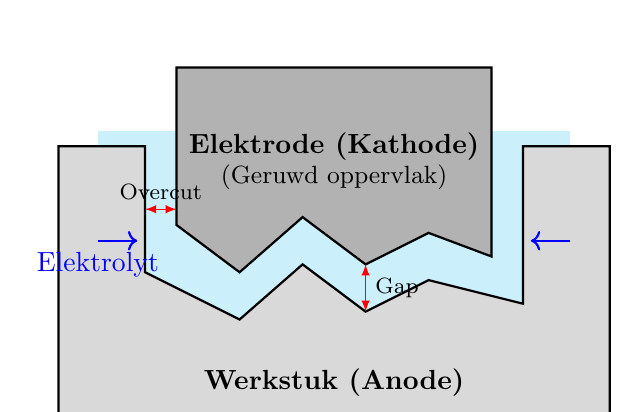
\begin{tikzpicture}
		% Styles
		\tikzset{
			tool/.style={fill=gray!60, draw=black, thick},
			workpiece/.style={fill=gray!30, draw=black, thick},
			electrolyte/.style={fill=cyan!20},
			dim/.style={draw=red, <->, >=latex, font=\footnotesize}
		}

		% Tool Coordinates (Rough bottom)
		\coordinate (T1) at (-2.0, 1.0);
		\coordinate (T2) at (-1.2, 0.4);
		\coordinate (T3) at (-0.4, 1.1);
		\coordinate (T4) at (0.4, 0.5);
		\coordinate (T5) at (1.2, 0.9);
		\coordinate (T6) at (2.0, 0.6);

		% Draw Electrolyte (Background in gap)
		\fill[electrolyte] (-3, -1) rectangle (3, 2.2);

		% Draw Tool
		\draw[tool] (-2, 3) -- (2, 3) -- (2.0, 0.6) -- (1.2, 0.9) -- (0.4, 0.5) -- (-0.4, 1.1) -- (-1.2, 0.4) -- (-2.0, 1.0) -- cycle;
		\node at (0, 2) {\textbf{Elektrode (Kathode)}};
		\node at (0, 1.6) {\small (Geruwd oppervlak)};

		% Draw Workpiece
		\draw[workpiece] (-3.5, 2.0) -- (-2.4, 2.0) -- (-2.4, 0.4) -- (-1.2, -0.2) -- (-0.4, 0.5) -- (0.4, -0.1) -- (1.2, 0.3) -- (2.4, 0.0) -- (2.4, 2.0) -- (3.5, 2.0) -- (3.5, -1.5) -- (-3.5, -1.5) -- cycle;
		\node at (0, -1) {\textbf{Werkstuk (Anode)}};

		% Dimensions / Annotations
		% Side Overcut
		\draw[dim] (-2.4, 1.2) -- (-2.0, 1.2) node[midway, above] {Overcut};
		% Bottom Gap
		\draw[dim] (0.4, -0.1) -- (0.4, 0.5) node[midway, right] {Gap};

		% Electrolyte flow
		\draw[->, blue, thick] (-3, 0.8) -- (-2.5, 0.8);
		\draw[->, blue, thick] (3, 0.8) -- (2.5, 0.8);
		\node[blue] at (-3, 0.5) {Elektrolyt};

	\end{tikzpicture}
	\caption{Schematische weergave van elektrochemisch bewerken (ECM) met een ruwe elektrode. De ontstane caviteit in het werkstuk is groter dan de elektrode door de "overcut" en de chemische werking.}
	\label{fig:ecm_overcut}
\end{figure}

Dit kan dus wel handig zijn bij zinkvonken. Het oppervlakte van vonkeroderen is een geharde laag door de opwarming en dan afkoeling van het materiaal.
EMC kan dit wegnemen en een goede oppervlaktekwaliteit geven.
Typische overcut-waarden bij ECM liggen tussen ongeveer 0,13 en 1,0 mm;
bij micro-ECM zijn waardes rond 0,02 mm mogelijk.
\newline

\subsection{Afnamen bij ECM}
\frm{Afnamesnelheid bij ECM}{M_{\mathrm{ECM}} = \dfrac{I \cdot A}{F \cdot V}\cdot \eta}{waarbij $M_{\mathrm{ECM}}$ de afnamesnelheid is [\si{g/s}], $I$ de stroomsterkte [\si{A}], $A$ de atoommassa [\si{g/mol}], $V$ de valentie [-], $F$ de Faraday-constante (\(96485\,\mathrm{C/mol}\)) en $\eta$ de efficiëntie [-].}
Voorbeeld bij Titaan:
A = 48A, V = 3, I = 2000A en \(\eta = 0.9\)
\[M_{ECM} = \dfrac{2000 \cdot 48}{96485 \cdot 3} \cdot 0.9 = 0.297 g/s\]
Omrekenen naar cm$^3$/min:
\[ \text{Dichtheid Titaan} = 4.51 g/cm^3 \]
\[ M_{ECM} = \dfrac{0.297 g/s}{4.51 g/cm^3} \cdot 60 s/min = 3.95 cm^3/min \]


\subsection{Toepassingen van ECM}
Je kunt ECM gebruiken voor:
\begin{itemize}
	\item Het bewerken van harde materialen zoals titanium en superlegeringen.
	\item Het maken van complexe vormen en fijne details die moeilijk te bereiken zijn met conventionele methoden.
	\item Het produceren van onderdelen met hoge oppervlaktekwaliteit zonder thermische of mechanische schade.
	\item Is gebruikt voor het maken van turbinebladen, raketonderdelen, medische implantaten, en micro-elektronische componenten.
\end{itemize}


\textbf{Afname zonder Stroom}
Je zet een masker op het werkstuk zodat alleen de delen die je wilt bewerken blootgesteld zijn aan de elektrolyt.
met je \textbf{Etsvloeistof} ga je de delen die dan geen masker hebben worden weggeërodeerd.
Je gaat iets meer wegnemen dan wat je wilt langs de binnenkant. Dit noemt \textbf{ondersnijding}.
\begin{figure}[ht]
	\centering
	\includegraphics[width=0.3\textwidth]{image75.png}
	\caption{Wegeroderen van materiaal zonder stroom met etsvloeistof}
	\label{fig:eroderen_etsvloeistof.png}
\end{figure}

De etstijd gaat bepalen hoeveel materiaal je wegneemt en de grote van de ondersnijding.
\newline

\textbf{Fotoetsen} is een gelijkaardig proces. Dit wordt vooral toegepast op
hele kleine delen. Je maskeert ook de oppervlakte met een laklaag.
Je legt dan nog een deel van transparante en niet transparante laag op.
UV-licht zal door de transparante laag gaan en de lak verwijderen.
Je kunt deze patronen dan etsen met een etsvloeistof.
Deze patronen kunnen enorm klein zijn, rond de micrometer.
Dit wordt toepast in micro-elektronica.
\newline
Net zoals bij normaal etsen krijg je ook ondersnijding waar je rekening mee moet houden.


\begin{figure}[ht]
	\centering
	\includegraphics[width=0.3\textwidth]{image73.png}
	\caption{Fotoetsen van een complex onderdeel met ECM}
	\label{fig:foto_etsen_ecm.png}
\end{figure}


\section{Ultrasoon bewerken (Ultrasonic Machining)}
Ultrasoon bewerken is een bewerkingsproces waarbij hoge-frequentie trillingen worden gebruikt om materiaal van een werkstuk te verwijderen.
Het proces maakt gebruik van een sonotrode die ultrasone trillingen (typisch tussen 20 kHz en 40 kHz) met een heel kleine amplitude genereert.
De trillingen creeëren kleine scheurtjes op het materiaaloppervlak en dan wordt dat materiaal uitgebroken.
Deze techniek werkt goed voor harde en bros materialen zoals keramiek, glas, en harde metalen omdat die niet
goed tegen scheurtjes kunnen. Je hammert dus als het ware op het materiaal met die ultrasone trillingen.

\begin{figure}[ht]
	\centering
	\includegraphics[width=0.4\textwidth]{image74.png}
	\caption{Principe van ultrasoon bewerken}
	\label{fig:principe_ultrasoon_bewerken.png}
\end{figure}

Ductiele materialen zoals metalen zijn ook bewerkbaar:
Door de enorm grote trillingen krijg je een \textbf{vermoeiingsproces} in het materiaal waardoor je ook materiaal kunt wegnemen.

\begin{figure}[ht]
	\centering
	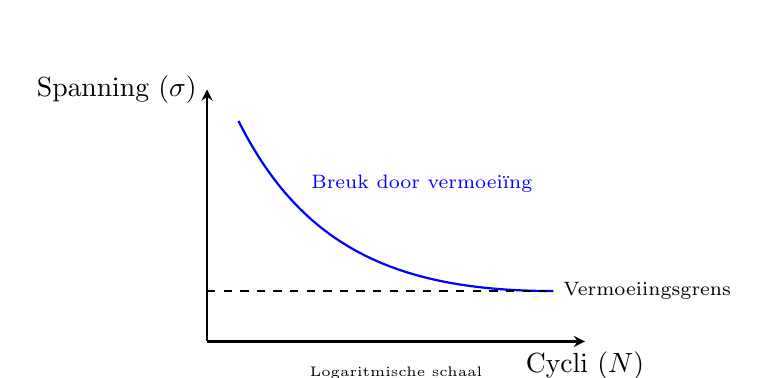
\begin{tikzpicture}[scale=0.8]
		% Axes
		\draw[thick,->,>=stealth] (0,0) -- (6,0) node[below] {Cycli ($N$)};
		\draw[thick,->,>=stealth] (0,0) -- (0,4) node[left] {Spanning ($\sigma$)};

		% Curve
		\draw[blue, thick] (0.5,3.5) .. controls (1.5,1.5) and (3,0.8) .. (5.5,0.8);

		% Annotations
		\node[blue, font=\scriptsize, anchor=west] at (1.5,2.5) {Breuk door vermoeiïng};
		\draw[dashed] (0,0.8) -- (5.5,0.8) node[right, font=\scriptsize] {Vermoeiingsgrens};

		% Labels
		\node[font=\tiny] at (3,-0.5) {Logaritmische schaal};
	\end{tikzpicture}
	\caption{S-N curve (Wöhler-curve) die het vermoeiingsproces bij metalen weergeeft.}
	\label{fig:vermoeiing_sn}
\end{figure}
\FloatBarrier

Het gegreedschap is gemaakt van harde materialen zodat het niet snel slijt.
\newline
Het wordt vooral toegepast op harde materialen die moeilijk te bewerken zijn met conventionele methoden.
\newline
Je kunt ook een profiel maken van het gereedschap en dan dat profiel in het werkstuk maken.
\newline


\section{Straalbewerkingen}
Straalbewerkingen zijn processen waarbij een geconcentreerde straal van energie of materiaal wordt gebruikt om materiaal van een werkstuk te verwijderen of te bewerken.


\begin{table}[ht]
	\centering
	\caption{Overzicht van verschillende straalbewerkingen.}
	\label{tab:straalbewerkingen}
	\begin{tabularx}{\textwidth}{|l|X|X|}
		\hline
		\textbf{Energiedrager} & \textbf{Bewerkingen}               & \textbf{Toepassingen}                                      \\
		\hline
		Vloeistof (Water)      & Waterstraalsnijden (WJM)           & Snijden van zachte materialen (plastic, textiel, voedsel). \\
		\hline
		Vloeistof + Abrasief   & Abrasief waterstraalsnijden (AWJM) & Snijden van harde materialen (metaal, glas, steen).        \\
		\hline
		Licht (Fotonen)        & Laserstraalbewerking (LBM)         & Snijden, lassen en boren van bijna alle materialen.        \\
		\hline
		Elektronen             & Elektronenstraalbewerking (EBM)    & Zeer nauwkeurig boren en snijden (in vacuüm).              \\
		\hline
		Ionen                  & Ionenstraalbewerking (IBM)         & Etsen op nanoschaal en oppervlaktebewerking.               \\
		\hline
		Gas / Plasma           & Plasmastralen (PAM)                & Ruw snijden van dikke metaalplaten.                        \\
		\hline
	\end{tabularx}
\end{table}

\subsection{Shotpeening}
Korrels worden met hoge snelheid op het oppervlak van een werkstuk geschoten.
Dit veroorzaakt plastische vervorming aan het oppervlak, wat leidt tot een verhoogde vermoeiingssterkte
door de inwendige spanningen die worden geïnduceerd.
\subsection{abrasief stralen}
Je gebruikt een straal van abrasieve deeltjes (zoals zand)
die met hoge snelheid op het oppervlak van een werkstuk worden gespoten.
Dit wordt vaak gebruikt voor het \textbf{reinigen, ontroesten of matten} van oppervlakken.
Het process werkt door de wet van bernoulli. (zie stromingen)
\theoriebox{Wet van Bernoulli}{
	In een stromend fluïdum is de som van de drukenergie, kinetische energie en potentiële energie per eenheid volume constant langs een stroomlijn:
	\[
		P + \frac{1}{2} \rho v^2 + \rho gh = \text{constant}
	\]
	waarbij \(P\) de druk is, \(\rho\) de dichtheid van het fluïdum, \(v\) de stroomsnelheid, \(g\) de zwaartekrachtversnelling en \(h\) de hoogte boven een referentieniveau.
}

Je deeltjes moeten hun kinetische energie kwijt kunnen op het oppervlakte.
Ze nemen dus materiaal weg.
\subsection{Waterstraalsnijden}
water wordt bij \textbf{4000 bar} door een kleine opening gepompt.
Deze kracht is om materiaal te snijden.
Je kunt hier dikke stukken materiaal mee wegsnijden.
\newline
Je hebt geen beinvloede zone, geen hitte dus geen TAZ.
Het is ook bruikbaar op andere industrieën zoals voedselindustrie.

\begin{figure}[ht]
	\centering
	\includegraphics[width=0.5\textwidth]{image76.png}
	\caption{Waterstraal snijden proces}
	\label{fig:image76.png}
\end{figure}

Een extra mogelijk is het gebruik van ijsbollejes om opervlakte te reinigen inplaats van zand.
Het ijs smelt gewoon weg en je moet geen zand opruimen.

\subsection{Laserstraalbewerking (LBM)}
\subsubsection{Hoe werk een laser?}
Een Laser is een geconcentreerde lichtbron die op één specifieke golflengte licht uitzendt met hoge intensiteit en coherentie.
\newline
\frm{Laser}{\textbf{L}ight \textbf{A}mplification by \textbf{S}timulated \textbf{E}mission of \textbf{R}adiation}{is een apparaat dat licht versterkt door gestimuleerde emissie van straling.}
Voor een laser te maken wordt materiaal hun atomen naar een hogere energietoestand gebracht door energie toe te voeren (pompproces).
Wanneer deze atomen terugvallen naar hun lagere energietoestand, zenden ze fotonen uit.
Dit process noemt \textbf{spontane emissie}.
\newline
Als deze fotonen andere aangeslagen atomen treffen,
kunnen ze deze atomen stimuleren om ook fotonen uit te zenden
die identiek zijn aan de oorspronkelijke fotonen (zelfde frequentie, fase en richting).
Dit process noemt \textbf{gestimuleerde emissie}.
\newline
Het resultaat is een coherente en monochromatische lichtstraal met hoge intensiteit.
\newline
\textbf{Workflow: Hoe een laser wordt gecreëerd}
\begin{figure}[ht]
	\centering
	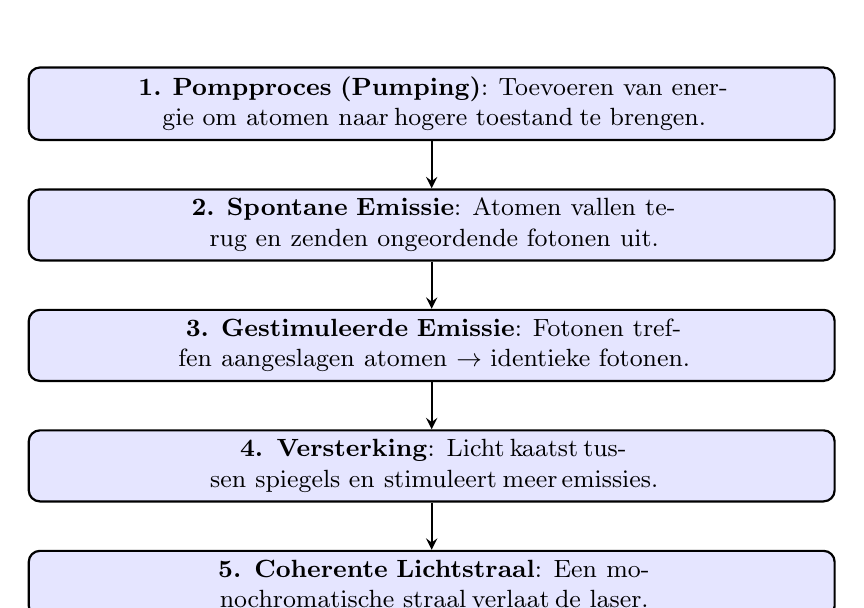
\begin{tikzpicture}[
			node distance=0.6cm and 2cm,
			block/.style={rectangle, draw, fill=blue!10, text width=10cm, text centered, rounded corners, minimum height=0.8cm, thick, font=\small},
			line/.style={draw, thick, ->, >=stealth}
		]
		% Nodes using relative positioning to avoid overlap
		\node (pumping) [block] {\textbf{1. Pompproces (Pumping)}: Toevoeren van energie om atomen naar hogere toestand te brengen.};

		\node (spontaneous) [block, below=of pumping] {\textbf{2. Spontane Emissie}: Atomen vallen terug en zenden ongeordende fotonen uit.};

		\node (stimulated) [block, below=of spontaneous] {\textbf{3. Gestimuleerde Emissie}: Fotonen treffen aangeslagen atomen $\to$ identieke fotonen.};

		\node (amplification) [block, below=of stimulated] {\textbf{4. Versterking}: Licht kaatst tussen spiegels en stimuleert meer emissies.};

		\node (output) [block, below=of amplification] {\textbf{5. Coherente Lichtstraal}: Een monochromatische straal verlaat de laser.};

		% Lines
		\draw [line] (pumping) -- (spontaneous);
		\draw [line] (spontaneous) -- (stimulated);
		\draw [line] (stimulated) -- (amplification);
		\draw [line] (amplification) -- (output);
	\end{tikzpicture}
	\caption{Stapsgewijze workflow van de werking van een laser.}
	\label{fig:laser_workflow_improved}
\end{figure}

\begin{figure}[ht]
	\centering
	\includegraphics[width=0.7\textwidth]{image77.png}
	\caption{Creeren van een laserstraal door gestimuleerde emissie.}
	\label{fig:creeren_laserstraal.png}
\end{figure}

De laserstraal heeft een paar problemen
\newline
Er wordt veel energie omgezet in warmte en de lichtkwaliteit moet je in
rekening houden.
\newline
Classificatie van lasers:
\begin{itemize}
	\item \textbf{Lasermedium:}
	      gas, vast, vloeistof, halfgeleider
	\item \textbf{Golfengte:}
	      infrarood, zichtbaar, ultraviolet
	\item \textbf{Aard van uitgaande straal:}
	      continue, gepulst
	\item \textbf{Het vermogen:}
	      van lasers in miliwat tot multi-kilowatt
	\item \textbf{Vorm lasercaviteit:}
	      langwerpig, rond, ringvormig, fiber en disklasers

	\item \textbf{De pompmethode:}
	      elektrisch, optisch
\end{itemize}

Lasers kunnen getransporteerd worden via lucht, glasvezel of spiegels.
Glasvezels kunnen ook lasers exiteren in de kabel.
Wanneer men spreekt over een fibrelaser betekent dat gewoon het medium die de laser doorbrengt.
\newline
\textbf{De golflengte $\lambda$} gaat je laser bepalen.
Kleinere golflengtes zijn preciezer maar zijn ook duurder te maken.
Vele lasertechnologie zijn recente ontwikkelingen (het jaar 2000).
Een yag laser is recent en door de korte golflengte kan je preciezer werken.
\newline
Hieronder zijn alle relevante type lasers voor het bewerken van materialen:
\begin{figure}[ht]
	\centering
	\includegraphics[width=0.8\textwidth]{Type_lasers.png}
	\caption{}
	\label{fig:Type_lasers.png}
\end{figure}

\textbf{absorbtie van laserlicht}
\newline
Je wilt zoveel mogelijk van de laserenergie laten absorberen door het werkstuk.
$R+T+A=1$ met R = reflectie, T = transmissie en A = absorptie.
Je wilt dus een hoge A hebben.
\newline

\begin{figure}[ht]
	\centering
	\includegraphics[width=0.4\textwidth]{Reflecteren in functie van de golflengte.png}
	\caption{}
	\label{fig:Reflecteren in functie van de golflengte.png}
\end{figure}
\FloatBarrier

In de figuur zie je dat bij staal dat 90 $\%$ van de CO2 laser wordt gereflecteerd. Niet zoals een YAG laser die maar 50 $\%$ reflecteert.
Hoe ze dit vroeger oploste was de CO2 laser met enorm grote vermogens gebruiken zodat er toch genoeg energie werd geabsorbeerd.
\newline

Deze verschillen in absorptie komt door de kristalstructuur/moleculaire structuur van het materiaal.

\begin{figure}[ht]
	\centering
	\includegraphics[width=0.4\textwidth]{Absorptie van polycarbonaat.png}
	\caption{}
	\label{fig:Absorptie van polycarbonaat.png}
\end{figure}

Bij kunststoffen is zoals polycarbonaat zie je dat bij een CO2 laser bijna alles wordt geabsorbeerd maar enorm veel gereflecteerd bij een YAG laser.
Bij deze toepassing wil je dus liever een CO2 laser gebruiken.

\subsubsection{kwaliteit van de laserstraal}
De BBP (Beam Parameter Product) is een maat voor de kwaliteit van een laserstraal.
\frm{BBP = Beam Parameter Product}{BBP = \omega_0 \cdot \dfrac{\theta}{2}}{waarbij $BBP$ het Beam Parameter Product is [\si{mm \cdot mrad}], \(\omega_0\) de straal van de bundeltaille (focuspunt) [\si{mm}] en $\theta$ de volledige divergentiehoek [\si{mrad}].}
Hoe kleiner $\theta$ is, hoe beter de kwaliteit van de laserstraal.

Je moet dus je laser focussen als je materiaal wilt bewerken.
Deze afstand moet precies zijn of je krijgt een groter focuspunt en dus minder intensiteit.

\begin{figure}[ht]
	\centering
	\includegraphics[width=0.5\textwidth]{Kwaliteit laserstraal.png}
	\caption{}
	\label{fig:Kwaliteit laserstraal.png}
\end{figure}

\textbf{Het intensiteitsprofiel van een laserstraal}
Een perfecte laser zou een perfecte cilinder zijn.
In de praktijk is dat niet zo. De laserintensiteit gaat een gaussiaans profiel hebben. -> Je intensiteitprofliel ziet er als volgt uit:

de intensiteit wordt gegeven door:
\[I = \frac{I_0}{e^{2}}\]
met I0 de maximale intensiteit in het midden van de bundel.

\begin{figure}[ht]
	\centering
	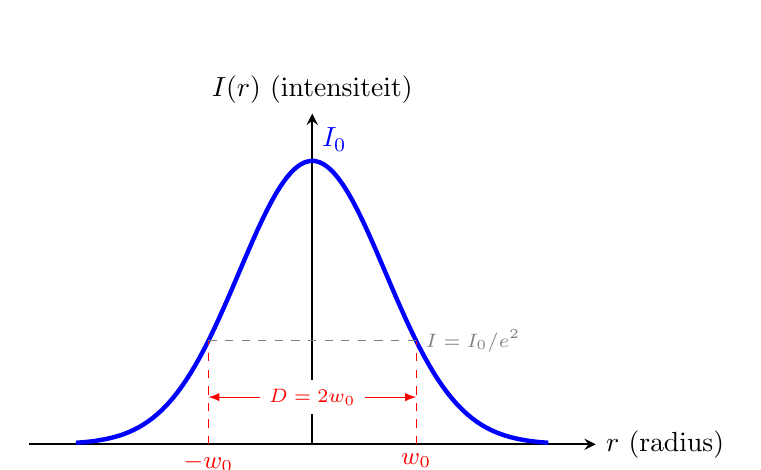
\begin{tikzpicture}[scale=1.2]
		% Assen
		\draw[thick,->,>=stealth] (-3,0) -- (3,0) node[right] {$r$ (radius)};
		\draw[thick,->,>=stealth] (0,0) -- (0,3.5) node[above] {$I(r)$ (intensiteit)};

		% Gaussiaanse curve (parabolische vorm nabij de top)
		\draw[ultra thick, blue, domain=-2.5:2.5, samples=100] plot (\x, {3*exp(-\x*\x/1.2)});

		% Annotaties
		\node[anchor=south west, blue] at (0,3) {$I_0$};

		% Bundelstraal w0 aanduiding
		% Bij x = 1.1 is de waarde ongeveer I0/e^2
		\draw[dashed, red] (-1.1, 0) -- (-1.1, {3*exp(-1.1*1.1/1.2)}) node[below, pos=0, font=\small] {$-w_0$};
		\draw[dashed, red] (1.1, 0) -- (1.1, {3*exp(-1.1*1.1/1.2)}) node[below, pos=0, font=\small] {$w_0$};
		\draw[<->, red, >=latex] (-1.1, 0.5) -- (1.1, 0.5) node[midway, fill=white, font=\scriptsize] {$D = 2w_0$};

		% Niveau I0/e^2
		\draw[dashed, gray] (-1.1, {3*exp(-1.1*1.1/1.2)}) -- (1.1, {3*exp(-1.1*1.1/1.2)}) node[right, font=\scriptsize] {$I = I_0/e^2$};

	\end{tikzpicture}
	\caption{Parabolische/Gaussiaanse intensiteitsverdeling van een laserbundel op het focuspunt.}
	\label{fig:laser_focus_intensity}
\end{figure}

voor een guassiaans profiel is het BBP:
\[BBP = \frac{\lambda}{\pi}\]
met $\lambda$ de golflengte van de laser.

Een kleinere golflengte $\lambda$ geeft dus een betere bundelkwaliteit van de laserstraal.

Om de bundel te focussen gebruik je een lens met een focuslengte \(f\).
De straal wordt dan gefocusseerd tot een straal met een straal \(w_0\) gegeven door:
\[w_0 = \frac{4 \lambda f}{\pi D}\]
Kleine verschillen in hoogte kan dus een groot verschil maken in de grootte van het focuspunt.
\begin{figure}[ht]
	\centering
	\includegraphics[width=0.5\textwidth]{Laserfocussen.png}
	\caption{Laserfocussen met verschillende focusafstanden \(f\).}
	\label{fig:Laserfocussen.png}
\end{figure}7

De $w_0$ kun je meten met warmtecamera's die de warmte van de laser opneemt. Hieruit kan je dan de BBP berekenen.

\subsubsection{Toepassingen}
\begin{itemize}
	\item \textbf{Snijden}: Het materiaal wordt lokaal gesmolten of verdampt door de hoge energiedichtheid, vaak ondersteund door een snijgas om de smelt te verwijderen.
	\item \textbf{Lassen}: Het verbinden van twee delen door ze op het contactvlak te smelten, wat resulteert in een smalle, diepe lasnaad met minimale thermische vervorming.
	\item \textbf{Boren}: Gebruik van korte laserpulsen met zeer hoge intensiteit om materiaal te verdampen en zo nauwkeurige gaten te creëren.
	\item \textbf{Oppervlaktebehandeling}: Aanpassen van de textuur of chemie van de toplaag, zoals het reinigen van oppervlakken of het creëren van specifieke ruwheidspatronen.
	\item \textbf{Harden}: Het lokaal verhitten van staal boven de kritische temperatuur,
	      gevolgd door zelf-afschrikking door de omringende koude massa, om de slijtvastheid te verhogen. Je kunt de randen van tandwielen harden zodat de punten sterker zijn.
	      Harden met een laser kreeg je minder deformatie als het harden in een oven.
	\item \textbf{Cladding}: Een laag van een ander materiaal (poeder of draad) op het werkstuk smelten om eigenschappen zoals corrosiebestendigheid of hardheid te verbeteren.
	\item \textbf{Solderen}: Het smelten van een toevoegmateriaal met de laser om een verbinding te maken, waarbij het basismateriaal zelf niet smelt (soldeerverbinding).
\end{itemize}

Afhankelijk van de toepassing met je de BBP en het vermogen aanpassen.

\subsubsection{machine gestuurde Lasers, NC lasers}
\begin{figure}[ht]
	\centering
	\includegraphics[width=0.8\textwidth]{NC-lasers.png}
	\caption{NC laser snijmachine}
	\label{fig:NC-lasers.png}

\end{figure}

\textbf{Belangrijke parameters bij laser snijden}
\newline
\textbf{Lasersmeltsnijden}: Snijgas (stikstof, argon) wordt tijdens het lasersnijden zodat de bewerking sneller afkloelt en dat er geen oxidatie optreedt en kans op brand verminderd.
De laser in een interte atmosfeer brengen zoals argon of stikstof kan ervoor zorgen dat je geen enkele oxidatie hebt.

\textbf{Laserbrandsnijden}: Je kunt ook het omgekeerde doen en zuurstof toevoegen om het snijproces te versnellen.

In beide gevallen is het belangrijk om het verwijderde materiaal (smelt) weg te blazen met het snijgas.

\subsubsection{Toepassingen}
Lasersnijden is snel en nauwkeurig en kan enorm kleine dingen maken.
\begin{figure}[ht]
	\centering
	\includegraphics[width=0.4\textwidth]{Kleinefiguurdoorlasersnijden.png}
	\caption{Toepassingen van lasersnijden in verschillende industrieën}
	\label{fig:Laser_toepassingen.png}
\end{figure}
\FloatBarrier
grote platen kun je ook snijden met lasers.

\subsubsection{Nadelen}
\begin{itemize}
	\item \textbf{Dross}: Tijdens het snijden kan er een ophoping van gesmolten materiaal aan de onderkant van het snijvlak ontstaan, wat resulteert in een ruwe afwerking die vaak nabewerking vereist.
	\item \textbf{burning defecten}: Bij het snijden van bepaalde materialen bij een te lage snijsnelheid, zoals bij kunststoffen, kan overmatige hitte leiden tot verbranding of verkoling langs de snijranden, wat de kwaliteit van het eindproduct vermindert.
	\item \textbf{Loss of full penetration}: Bij het snijden van dikkere materialen kan het voorkomen dat de laserstraal niet volledig door het materiaal heen dringt, wat resulteert in onvolledige sneden die opnieuw bewerkt moeten worden.
	\item \textbf{Aanhechting van gesmolten materiaal}: Bij brandsnijden aan hoge snijsnelheden kan gesmolten materiaal aan de snijkant blijven plakken, wat leidt tot onregelmatige randen en mogelijke structurele zwaktes in het gesneden onderdeel.
\end{itemize}

\begin{warningbox}[title=EXAMEN CHECKLIST: NIET-CONVENTIONELE BEWERKINGEN]
    \begin{itemize}
        \item \textbf{EDM vs. ECM}: Ken het fundamentele verschil (thermisch vs. chemisch) en de vloeistof (diëlektricum vs. elektrolyt).
        \item \textbf{EDM Fases}: Begrijp de cyclus: ontbranding $\to$ ontlading (plasma) $\to$ implosie (swarf afvoer).
        \item \textbf{EDM Slijtage}: Begrijp waarom de elektrode wel slijt bij EDM (ionenbombardement) maar niet bij ECM.
        \item \textbf{ECM Afname}: Leg uit waarom de afnamesnelheid afhangt van de stroom ($I$) en de atoommassa, niet van de hardheid van het materiaal.
        \item \textbf{Laser}: Begrijp de energiebalans ($A+R+T=1$) en waarom golflengte cruciaal is voor materiaalkeuze.
        \item \textbf{Ultrasoon}: Weet dat dit ideaal is voor brosse materialen (keramiek) door microscheur-initiatie.
    \end{itemize}
\end{warningbox}

\chapter{Scheiden}

\begin{conceptbox}[title=Knippen vs. Ponsen]
    \begin{itemize}
        \item \textbf{Knippen}: Scheiden langs een open lijn (meestal recht) met twee langs elkaar bewegende messen.
        \item \textbf{Ponsen}: Scheiden langs een gesloten contour met behulp van een stempel en een matrijs.
    \end{itemize}
\end{conceptbox}

Bij Scheiden ga je knippen of ponsen. Hierbij heb je geen spanen.
Je kunt alle vorige technieken gebruiken om te scheiden.
Het afgenome materiaal is dus nog steeds bruikbaar.
\newline
\section{Ponsen en knippen}
Bij Ponsen ga je met een gesloten profiel een gat maken in een plaat.
\newline
Bij knippen ga je met een rechte snede je materiaal scheiden.
\newline
\subsection{Algemeen Knippen en Ponsen}:
Je gaat pas vervorming krijgen als je plastisch gaat vervormen.
Om het te vervormen heb je een afschuifkracht.
\newline
\frm{Afschuifkracht bij ponsen}{\ensuremath{F_{th} = \tau_{max} \cdot L \cdot s_0}}{Waarbij 
\(\!F_{th}\!\) de afschuifkracht is [\si{N}], \(\tau_{max}\) de maximale schuifspanning [\si{N/mm^2}],
	\(L\) de omtrek van het profiel [\si{mm}] en \(s_0\) de plaatdikte [\si{mm}].}

Je materiaal gaat afschuiven tot dat het doorbreekt en dan het je je materiaal verwijderd.

\begin{figure}[ht]
	\centering
	\includegraphics[width=0.45\textwidth]{Kracht-wegdiagram van Ponsen.png}
	\includegraphics[width=0.45\textwidth]{Het Ponsprocess.png}
	\caption{}
	\label{fig:Kracht-wegdiagram van Ponsen.png}
\end{figure}
\FloatBarrier
Je ziet bij de grafiek dus eerst verhogingen van de kracht. Dit is de schuifkracht, het bereikt dan een piekbelasting.
Daarna gaat de kracht dalen omdat het materiaal begint te breken.
De Z-waarde is hier de afstand dat het stuk beweegt tot dat het doorbreekt.
\newline

Bij knippen en ponsen heb je drie fases:
\begin{enumerate}
	\item \textbf{Elastische vervorming}: Het materiaal ondergaat een tijdelijke vervorming die verdwijnt wanneer de kracht wordt verwijderd.
	\item \textbf{Plastische vervorming}: Het materiaal begint permanent te vervormen zodra de vloeigrens is overschreden.
	\item \textbf{De scheidingsfase}: Uiteindelijk bereikt het materiaal zijn breekpunt, wat resulteert in het scheiden van het materiaal.
\end{enumerate}

De vorm en kwaliteit van de snede hangt af van de breette van de snijpleet.
\begin{figure}[ht]
	\centering
	\includegraphics[width=0.45\textwidth]{image80.png}
	\caption{Afschuiving door knippen}
	\label{fig:image80.png}
\end{figure}



\subsection{Knippen}
Knippen is een spaanloze bewerking.
Je hebt inplaats van een spaanhoek een snijhoek $\gamma$ en een vrijloophoek $\alpha$.
Een voorbeeld van een knipmachine is een guillotineschaar.
\frm{Schuifkracht bij knippen}{\ensuremath{F = 0.5 \cdot \dfrac{s^2}{\tan\varepsilon} \cdot \tau}}{waarbij \(F\) de afschuifkracht is [\si{N}], \(s\) de plaatdikte [\si{mm}], \(\varepsilon\) de snijhoek [$^\circ$] en \(\tau\) de schuifspanning van het materiaal [\si{N/mm^2}].}

De \textbf{snijspeelt} is de afstand tussen het mes en het tegenmes.
Als deze niet goed is ingesteld krijg je slechte sneden.
\newline
Dit is de rede waarom versleten scharen slechte sneden geven.

\begin{figure}[ht]
	\centering
	\includegraphics[width=0.8\textwidth]{snijspleetbelang.png}
	\caption{Het belang van de juiste snijspleet bij knippen}
	\label{fig:snijspleetbelang.png}
\end{figure}

Nog voorbeelden van knipmachines zijn:
\begin{itemize}
	\item \textbf{strokenschaar} - Een knipmachine speciaal ontworpen voor het verwerken van langwerpige stroken metaal. Deze machines zijn ideaal voor het afkorten van platen tot breedte en maken lange, rechte sneden met hoge precisie.

	\item \textbf{rolschaar} - Een knipmachine die werkt met twee tegenover elkaar geplaatste, ronddraaiende messen. Hierdoor wordt een continue knipvorming gecreëerd wat bijzonder geschikt is voor het produceren van lange rechte sneden en het verwerken van dikke platen met minder krachtinspanning.

	\item \textbf{figuurschaar} - Een geavanceerde knipmachine in staat om complexe vormen en contouren te snijden. Deze machines worden vaak CNC-gestuurd en kunnen zowel rechte als gebogen sneden maken, ideaal voor het produceren van op maat gemaakte onderdelen en profielen.
\end{itemize}


\subsection{Ponsen}
Ponsen is ook een spaanloze bewerking. Een simpel voorbeeld is een perforator.

\frm{Eerste formule Schuifkracht bij ponsen}{\ensuremath{F = s_0 \cdot l \cdot \tau}}
{waarbij \(F\) de afschuifkracht is [\si{N}], \(s_0\) de plaatdikte [\si{mm}], \(l\) de omtrek van het profiel [\si{mm}] en \(\tau\) de schuifspanning van het materiaal [\si{N/mm^2}].}

Bij ponsen is er geen enkele opbouw. Je hebt direct een indrukking en dus snel een vergroting
van de schuifspanningen.

\begin{figure}[ht]
	\centering
	\includegraphics[width=0.45\textwidth]{Schuifspanningen bij Ponsen.png}
	\caption{Ponsen proces met de verschillende fases}
	\label{fig:Ponsen proces.png}
\end{figure}
\FloatBarrier

De eerste formule is een benadering.
Een betere formule is:
\frm{Tweede formule Schuifkracht bij ponsen}{\ensuremath{F = 1.1 \cdot y_s \cdot s_0 \cdot l \cdot \tau \cdot k_s}}
{waarbij \(F\) de afschuifkracht is [\si{N}], \(y_s\) een correctiefactor [-], \(\tau\) de schuifspanning [\si{N/mm^2}],
	\(s_0\) de plaatdikte [\si{mm}], \(l\) de omtrek [\si{mm}] en \(k_s\) de specifieke snijkracht [-].}

\textbf{$k_s$ de specifieke snijkracht}
\newline
De specifieke snijkracht \(k_s\) is een maat voor de kracht die nodig is om een eenheid van materiaal te snijden.
Het wordt uitgedrukt in N/mm\(^2\) en hangt af van het materiaaltype en de dikte van het werkstuk.
\[
	k_s = X_f \cdot R_m
\]
met \(X_f\) de snijfactor en \(R_m\) de treksterkte van het materiaal.



\subsection{Fijnstancen}

\begin{conceptbox}[title=Fijnstansen]
    Fijnstansen is een precisie-ponsproces waarbij de snijspleet extreem klein is ($<1\%$ van de plaatdikte) en het materiaal volledig wordt vastgeklemd. Dit resulteert in een volledig glad snijvlak over de hele dikte, zonder de typische breukzone van normaal ponsen.
\end{conceptbox}

Fijnstancen is snijden en ponsen met een heel kleine
snijspleet. rond de 1-0.01mm.
Bij normaal ponsen en knippen heb je ruimte 
rond je snede langs boven. De tool zijn hoek werd 
op dezelfde hoek gelegt als de onderplaat en zo werd er gesneden of geponst.
\newline
Bij fijnstancen heb je geen ruimte meer. 
De plaat wordt dus volledig vastgeklemd tussen de boven en onderplaat
en de pons wordt dan heel precies geleid.
e snijspleet is klein maar is ook constant.
\newline
\begin{figure}[ht]
    \centering
    \includegraphics[width=0.8\textwidth]{Fijnsnijden.png}
    \caption{}
    \label{fig:Fijnsnijden.png}
\end{figure}

Het is duurder om te zien maar je oppervlaktekwaliteit van 
je afbreukzone is veel beter. Beter dan lasersnijden en normaalponsen.

\subsection{Volgsnijstempel}
Bij volgsnijstempel heb je een soort lopende band van ponsen.
Stel je wilt een sleutelgat maken. Je gaat stap per stap vier gaten maken op een lange plaat aluminium sheet.
en dan het sleutelgat. De plaat kan blijven bewegen zodat je snel velle producten kunt maken.
Je verdeeld verschillende operaties over verschillende stempels.
Deze stempels zijn niet alleen voor door te ponsen maar kunnen ook 
het product een bepaald oppervlakte geven.
\newline
Deze techniek wordt gebruikt wanneer je grote aantallen van een product moet maken.
De stempels (gemaakt uit hard staal met wolframcarbide) zijn duur maar je kunt er wel enorm snel mee werken.

\textbf{Examenvraag}
\newline
Hoe zou je de geleiders maken voor een volgsnijstempel?
\newline
Met draadvonken kun je heel precies openingen uit hardmetaal maken in dezelfde vorm als de stempel.
Je maakt de toppen van de geleiders uit keramiek zodat ze niet slijten.
\subsection{Revolvermachine}
Je kunt computergestuurd ponsen op een grote aluminium plaat.
Je plaat kan rondbewegen langs de x-en y-as en de pons kan operaties doen.
Dit gaan enorm snel.
Het is sneller dan een lasersnijmachine dus als je grote aantallen moet maken is dit ideaal.

\subsection{Knabbelen}

Bij knabbelen ga je rond een contour ponsen om iets uit te knippen.
Afhankelijk van de stapgrootte tussen de ponsen krijg je een grovere of fijnere rand.
Dit is enorm snel, rond 10 slagen per seconde.
\begin{figure}[ht]
  \centering
  \includegraphics[width=0.4\textwidth]{Ruw oppervlakte Knappelen.png}
  \caption{}
  \label{fig:Knabbelen.png}
\end{figure}
\FloatBarrier
De pons kun je combineren met verschillende vormen: cirkel, vierkant, driehoek enz.
\newline

\section{Mechanisch Scheiden, verspannen}
Bij mechanisch scheiden ga je materiaal wegnemen door te verspannen.
Je gaat niet de structuur van je materiaal veranderen. 
Je hebt verschillende technieken:
\begin{itemize}
  \item \textbf{Zagen}: Gebruik van een zaagblad met tanden om materiaal te verwijderen door middel van een snijbeweging.
  \item \textbf{Schuren}: Verwijderen van materiaal met schuurpapier of schuurbanden door wrijving.
  \item \textbf{Slijpen}: Gebruik van een slijpschijf om materiaal te verwijderen en een glad oppervlak te creëren.
  \item \textbf{Polijsten}: Fijnere afwerking van oppervlakken door gebruik van polijstmiddelen en doeken.
  \item \textbf{Boren}: Creëren van ronde gaten in materialen met behulp van een boor.
\end{itemize}


\section{Fysische scheiding}
Bij fysische scheiding ga je materiaal wegnemen door fysische processen.
Je hebt opnieuw verschillende technieken:
\begin{itemize}
  \item \textbf{Brandnsijden}: Metaal snijden door verbranding met behulp van een zuurstofstraal.
  Het materiaal wordt verhit tot boven de ontbrandingstemperatuur en vervolgens wordt zuurstof toegevoegd om het metaal te oxideren en weg te blazen.
  Als je te weinig zuurstof gebruikt krijg je aanhechting van gesmolten materiaal.
  Als je te veel zuurstof gebruikt krijg je een ruwe rand en een te grote snijholte.
  \item \textbf{Draadvonken}: Gebruik van elektrische vonken tussen een elektrode en het werkstuk om materiaal te verwijderen.
  \item \textbf{Stralen}: Gebruik van abrasieve deeltjes om materiaal te verwijderen of oppervlakken te reinigen.
  \item \textbf{Laser snijden}: Gebruik van een geconcentreerde laserstraal om materiaal te smelten of te verdampen.
  \item \textbf{Waterstraalsnijden}: Gebruik van een hogedruk waterstraal om materiaal te snijden zonder thermische effecten.
  \item \textbf{Plasmasnijden}: Gebruik van een plasmaboog om metaal te snijden door het te verhitten en te smelten.
  Plasma creert een vlam van geïoniseerd gas die extreem heet is.
\end{itemize}

\begin{table}[ht]
    \centering
    \caption{Vergelijking van scheidingsprocessen}
    \label{tab:scheidingsprocessen}
    \scriptsize
    \setlength{\tabcolsep}{3pt}
    \begin{tabularx}{\textwidth}{@{} l >{\raggedright\arraybackslash}X l >{\raggedright\arraybackslash}X c c @{}}
        \toprule
        \textbf{Processen} & \textbf{Toepassing} & \textbf{Snelheid} & \textbf{Voor- en nadelen} & \textbf{Nauwk.} & \textbf{WBZ} \\
         & & & & \textbf{(mm)} & \textbf{(mm)} \\
        \midrule
        Knippen & Plaat 0,2--10mm & lengte/knip & + grote lengten \newline -- bramen & $>0,1$ & -- \\
        \addlinespace
        Ponsen & Plaat 0,2--10mm & $\le$ 30 sl/s & + massa \newline -- bramen & $>0,1$ & -- \\
        \addlinespace
        Knabbelen & Plaat 0,2--10mm & $\le$ 0,1 m/s & + massa/kl. prod. \newline + contouren \newline -- bramen/ruw & 0,1 & -- \\
        \addlinespace
        Uitsnijden & Plaat 0,2--3mm & $\le$ 30 sl/s & + massa \newline + kleine prod. & 0,05 & -- \\
        \addlinespace
        Zagen & Plaat/buis/staf $>1$mm & $\le$ 0,05 m/s & + enk. st./massa \newline -- bramen & $>0,3$ & -- \\
        \addlinespace
        Doorslijpen & Harde mat. (tot 90mm) & ? & + enk. st./massa \newline -- bramen & 0,05 & $<0,1$ \\
        \addlinespace
        Omtrekfrezen & Platen (tot 12mm) & ? & + glad contour \newline -- enk. stuks & 0,05 & -- \\
        \addlinespace
        Waterstraal- & Plaat/buis/staf $>1$mm & $\le$ 0,08 m/s & + flexibel/geen WBZ \newline + enk. st./series \newline -- lawaai & 0,1 & -- \\
        snijden & & & & & \\
        \addlinespace
        Brandsnijden & Staal $>500$mm, buis & $\le$ 0,05 m/s & + flexibel \newline + enk. st./series \newline -- lawaai/WBZ & $>0,5$ & $>2$ \\
        \addlinespace
        Plasmasnijden & Geleidende mat. $>10$mm & $\le$ 0,2 m/s & + flexibel \newline + enk. st./series \newline -- WBZ & 0,5 & $>1$ \\
        \addlinespace
        Lasersnijden & Plaat/buis/prof. $\le$ 5mm & $\le$ 0,2 m/s & + flexibel/kwaliteit \newline + enk. st./series \newline + kleine WBZ & 0,2 & $>0,1$ \\
        \addlinespace
        Draadvonken & Harde geleidende mat. & $\le$ 0,7 mm$^2$/s & + flexibel \newline + enk. st./series \newline + kwaliteit & 0,05 & $<0,1$ \\
        \bottomrule
    \end{tabularx}
\end{table}

Deze tabel is enorm belangrijk want hij kan vragen. Welke van deze technieken zijn het 
snelste, goedkoopste, meest precieze enz.

Je ziet dat enorm veel technieken die we al gezien hebben terugkomen bij dit hoofdstuk. 
Niet echt super handig maar het is een goede herhaling.

\begin{warningbox}[title=EXAMEN CHECKLIST: SCHEIDEN]
    \begin{itemize}
        \item \textbf{Ponsen \& Knippen}: Begrijp het proces (elastisch $\to$ plastisch $\to$ breuk) en de invloed van de snijspleet.
        \item \textbf{Schuifkracht}: Ken de formule $F = \tau \cdot L \cdot s_0$ en weet hoe de snijhoek de kracht vermindert.
        \item \textbf{Fijnstansen}: Leg uit waarom de precisie hier veel hoger is en ken de noodzaak voor een drievoudige krachtwerking.
        \item \textbf{Volgsnijstempel}: Begrijp het principe van opeenvolgende bewerkingen in één matrijs voor massaproductie.
        \item \textbf{Brandsnijden}: Weet dat dit een chemisch proces is (oxidatie) en ken de beperkingen (grote TAZ, ruwe rand).
    \end{itemize}
\end{warningbox}

\chapter{Oervormen (Gieten van metalen)}

\begin{conceptbox}[title=Slink vs. Krimp]
    \begin{itemize}
        \item \textbf{Slink}: Volumevermindering tijdens de faseovergang van vloeibaar naar vast. Dit wordt gecompenseerd door \keyterm{opkomers} (voedingsreservoirs).
        \item \textbf{Krimp}: Volumevermindering tijdens de verdere afkoeling van het gestolde metaal naar kamertemperatuur. Dit wordt gecompenseerd door de \keyterm{krimptoeslag} op het model.
    \end{itemize}
\end{conceptbox}

\section{Inleiding}

\begin{conceptbox}[title=Directionele stolling]
    Om slinkholtes te voorkomen, moet het gietstuk zo ontworpen zijn dat de stolling begint bij de dunste delen en eindigt bij de opkomer. De opkomer moet als laatste stollen om het krimpend metaal in het gietstuk aan te vullen.
\end{conceptbox}

Bij oervormen ga je een vormloos materiaal (vloeistof, pasta, poeder) in een profiel gieten 
en dan laten afkoelen en stollen zodat het zijn vorm behoudt.
In dit hoofdstuk hebben we het vooral over metaalgieten.
Metaalgieten is al eeuwenoud en is toegepast in het oude Rome, China enz.

Je gaat vaak meerdere stukken gieten.
Je hebt ook enorm veel vrijheid in de vorm die je kunt gieten.

De materialen die we kunnen gebruiken:
\begin{itemize}
	\item ferro-materialen: lamellair gietijzer, nodulair gietijzer, gietstaal, enz. 
	\item niet-ferro-materialen: aluminiumlegeringen, koperlegeringen, magnesiumlegeringen, titaniumlegeringen, enz.
	\item niet-metalen: kunststoffen, keramiek, composieten, enz.
\end{itemize}

Je hebt dus een grote keuze aan materialen.

\begin{figure}[ht]
	\centering
	\includegraphics[width=0.8\textwidth]{Tabel van soorten legeringen die gegoten worden.png}
	\caption{Tabel van soorten legeringen die gegoten worden.}
	\label{fig:Tabel van soorten legeringen die gegoten worden.png}
\end{figure}

De stappen om een gietstuk te maken zijn:
\begin{enumerate}
	\item Smelten van materiaal
	\item Vullen van een vormholte -> afkoeling van het materiaal
	\item Uitnemen van het stuk
\end{enumerate}

\begin{conceptbox}
	\textbf{Volumevermindering bij stollen}
	Volumevermindering door stollen noemt men \textbf{Slink}. Een slink is een microscopisch gaatje in het gietstuk dat ontstaat tijdens het stollen en wordt gecompenseerd door opkomers.
	Dit zijn extra stukken materiaal die je toevoegt aan je gietstuk.

	De volumevermindering door het afkoelen noemt men \textbf{Krimp}. -> gecompenseerd door krimptoeslag.
	Dit is een extra maat die je aan je gietstuk toevoegt zodat het na afkoeling de juiste maat heeft.

	De krimphoeveelheid hangt af van:
	\begin{itemize}
		\item de geometrie
		\item legering
	\end{itemize}
	Grotere stukken krimpen meer dan kleine stukken.
\end{conceptbox}

\subsection{Maken van een vormholte}
Je hebt twee soorten vormen:
\begin{itemize}
	\item \textbf{Permanent vormen}: Je kunt deze vormen meerdere keren gebruiken. Gemaakt uit metaal.
	\item \textbf{Eenmalige vormen}: Je kunt deze vormen maar één keer gebruiken. Gemaakt uit zand of keramiek.
\end{itemize}
\textbf{Eenmalige vormen:}

Je gaat je vorm maken uit zand en dan gieten in het zand. 
Je verwijdert dan het zand maar dan gaat je vorm verloren.

\textbf{Permanent vormen:}

Je gaat je vorm maken uit metaal.
Je kunt dan spuitgieten, coquillegieten of andere speciale giettechnieken gebruiken.

De keuze hangt af van de smelttemperatuur waarmee je gaat gieten.

\section{Gieten in zand}
Gieten in zand is niet heel precies maar er is geen limiet aan de grootte van het product dat je kunt maken 
en het is goedkoop. In de industrie gaan ze dus vaak voor zandgieten en daarna nabewerken om de ruwheid en precisie te verbeteren.
Het zand dat ze gebruiken is niet echt zand maar een mengsel van zand, klei en water die steviger is dan gewoon zand.

\begin{figure}[ht]
	\centering
	\includegraphics[width=0.45\textwidth]{Zandgieten.png}
	\caption{Zandgieten proces: maken van eenmalige zandvormen voor metaalgieten}
	\label{fig:Zandgieten proces.png}
\end{figure}
\FloatBarrier

\begin{center}
	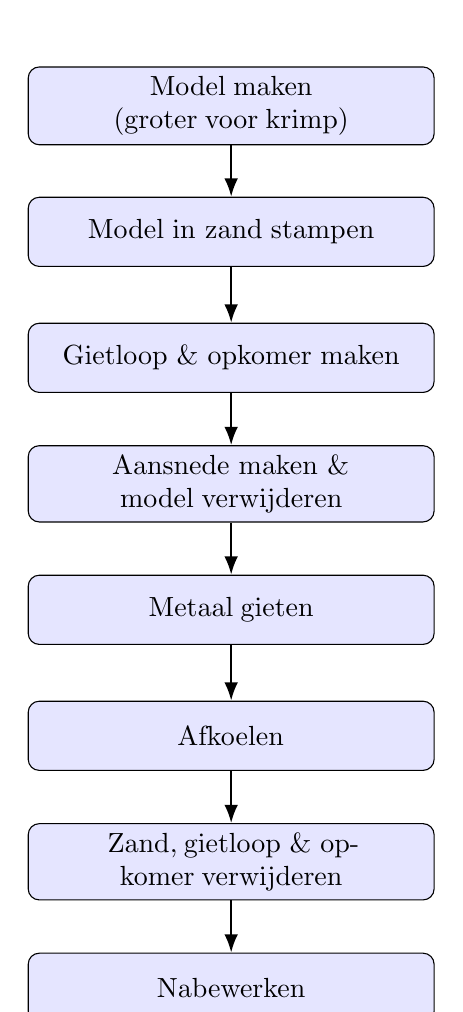
\begin{tikzpicture}[node distance=1.6cm, auto,
		block/.style={rectangle, draw, rounded corners, fill=blue!10, text width=14em, align=center, minimum height=2.5em},
		line/.style={draw, -Latex, thick}]
		% Nodes
		\node [block] (model) {Model maken\\(groter voor krimp)};
		\node [block, below of=model] (zand) {Model in zand stampen};
		\node [block, below of=zand] (kanalen) {Gietloop \& opkomer maken};
		\node [block, below of=kanalen] (aansnede) {Aansnede maken \& model verwijderen};
		\node [block, below of=aansnede] (gieten) {Metaal gieten};
		\node [block, below of=gieten] (afkoelen) {Afkoelen};
		\node [block, below of=afkoelen] (verwijderen) {Zand, gietloop \& opkomer verwijderen};
		\node [block, below of=verwijderen] (nabewerken) {Nabewerken};

		% Paths
		\path [line] (model) -- (zand);
		\path [line] (zand) -- (kanalen);
		\path [line] (kanalen) -- (aansnede);
		\path [line] (aansnede) -- (gieten);
		\path [line] (gieten) -- (afkoelen);
		\path [line] (afkoelen) -- (verwijderen);
		\path [line] (verwijderen) -- (nabewerken);
	\end{tikzpicture}
\end{center}

Het model moet iets groter zijn dan het uiteindelijke product om krimp te compenseren. 
Nadat het model in het zand is gestampt, wordt er een aansnede gemaakt in de bovenkant van de zandvorm zodat het model verwijderd kan worden. 
Na het gieten en afkoelen wordt het zand verwijderd en worden de gietloop en opkomer afgebroken.

\begin{conceptbox}
	\textbf{Gietloop en opkomer}

	De \textbf{gietloop} is het kanaal waardoor het gesmolten metaal in de vormholte stroomt.
	Het ontwerp van de gietloop is cruciaal om een gelijkmatige vulling van de vorm te garanderen en om turbulentie te minimaliseren, wat kan leiden tot defecten in het gietstuk.

	De \textbf{opkomer} is een extra reservoir dat is verbonden met de vormholte en dient als een bron van extra metaal tijdens het stollingsproces.
	Dit helpt om volumevermindering door \textbf{slink} te compenseren en voorkomt het ontstaan van holtes of insluitingen in het uiteindelijke gietstuk.
	De opkomer helpt ook de operator te laten zien of het gietstuk volledig is gevuld.
\end{conceptbox}

\subsection{slink, krimp en lossing}
\begin{conceptbox}
	\begin{enumerate}
		\item \textbf{Slink}: Volumevermindering door stollen. Gecompenseerd door opkomers.
		\item \textbf{Krimp}: Volumevermindering door afkoelen. Gecompenseerd door krimptoeslag.
		\item \textbf{Lossing}: Het proces van het verwijderen van het gietstuk uit de vorm.
		      Belangrijk om te zorgen dat het gietstuk niet beschadigd raakt tijdens het verwijderen.
	\end{enumerate}
\end{conceptbox}

Om deze dingen te voorkomen zetten we opkomers. Materialen kunnen complexe geometrie hebben. 
Soms moet je dus meerdere opkomers zetten zodat de vorm overal goed gevuld wordt.

\begin{figure}[ht]
	\centering
	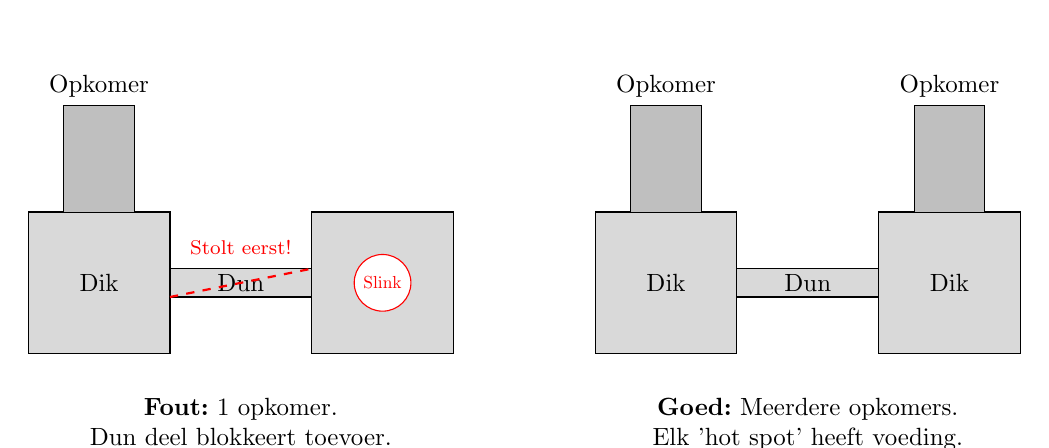
\begin{tikzpicture}[scale=0.9, every node/.style={transform shape}]
		% Bad scenario
		\begin{scope}[xshift=0cm]
			% Casting parts 
			\draw[fill=gray!30] (0,0) rectangle (2,2) node[midway] {Dik};
			\draw[fill=gray!30] (2,0.8) rectangle (4,1.2) node[midway] {Dun};
			\draw[fill=gray!30] (4,0) rectangle (6,2) node[midway] {Dik};

			% Riser on left only
			\draw[fill=gray!50] (0.5,2) -- (0.5,3.5) -- (1.5,3.5) -- (1.5,2);
			\node[above] at (1,3.5) {Opkomer};

			% Solidification/Defect
			\draw[dashed, red, thick] (2,0.8) -- (4,1.2); % Blockage indication
			\node[text=red, font=\footnotesize, align=center] at (3,1.5) {Stolt eerst!};

			\draw[fill=white, draw=red] (5,1) circle (0.4) node[scale=0.7, text=red] {Slink};

			\node[below=0.5cm, align=center] at (3,0) {\textbf{Fout:} 1 opkomer.\\Dun deel blokkeert toevoer.};
		\end{scope}

		% Good scenario
		\begin{scope}[xshift=8cm]
			% Casting parts 
			\draw[fill=gray!30] (0,0) rectangle (2,2) node[midway] {Dik};
			\draw[fill=gray!30] (2,0.8) rectangle (4,1.2) node[midway] {Dun};
			\draw[fill=gray!30] (4,0) rectangle (6,2) node[midway] {Dik};

			% Riser on left 
			\draw[fill=gray!50] (0.5,2) -- (0.5,3.5) -- (1.5,3.5) -- (1.5,2);
			\node[above] at (1,3.5) {Opkomer};

			% Riser on right
			\draw[fill=gray!50] (4.5,2) -- (4.5,3.5) -- (5.5,3.5) -- (5.5,2);
			\node[above] at (5,3.5) {Opkomer};

			\node[below=0.5cm, align=center] at (3,0) {\textbf{Goed:} Meerdere opkomers.\\Elk 'hot spot' heeft voeding.};
		\end{scope}
	\end{tikzpicture}
	\caption{Directionele stolling: dunne secties stollen sneller en kunnen de toevoer naar dikkere secties afsluiten, wat meerdere opkomers noodzakelijk maakt.}
	\label{fig:meerdere_opkomers}
\end{figure}

Wanneer een gietstuk bestaat uit dikke delen die verbonden zijn door dunnere secties, 
treedt een probleem op bij het stollen.
De dunnere sectie zal sneller stollen dan de dikke delen (vanwege een lagere modulus $V/A$). 
Als dit gebeurt, wordt de toevoer van vloeibaar metaal vanuit de centrale opkomer naar het achterliggende dikke deel afgesneden. 
Omdat dit dikke deel nog vloeibaar is en krimpt tijdens het verdere stollingsproces,
maar geen vers metaal meer kan ontvangen, ontstaat er een vacuüm of \textbf{slinkholte}. 

Om dit te verhelpen, moet elk geïsoleerd dik deel (hot spot) voorzien worden van zijn eigen opkomer, 
zodat directionele stolling naar de opkomer toe gewaarborgd blijft.

Je kunt hiervoor ook compenseren tijdens het ontwerpen zodat dit geen factor is. 

Vandaag de dag zijn er ook computersimulaties om te zien hoe je gietstuk gaat stollen.

\subsection{Hoe complexe modellen uit het zand halen?}
Bij complexe modellen kun je het niet uit het zand verwijderen zonder de zandvorm te beschadigen.
Je gaat hiervoor twee subdelen maken die je op elkaar gaat zetten.
Je maakt een bovenkant en een onderkant. We noemen deze dingen \textbf{Vormkasten}

Deze delingen kunnen specifiek op je model worden aangepast.

\subsection{Kernen}
Je kunt inwendige holtes maken door toepassing van \textbf{kernen}.
Dit zijn stukken zand die je in de vormholte plaatst voordat je gaat gieten zodat je gaten hebt in je product.
\begin{figure}[ht]
	\centering
	\includegraphics[width=1\textwidth]{Kernen_gieten.png}
	\caption{Kernen bij gieten}
	\label{fig:Kernen_gieten.png}
\end{figure}

Je neemt de buitenkant van het product eerst en je plaatst dan je kern in het gietstuk.
Dit is wel wat werk want je moet bij elke keer dat je giet dit herhalen. Vandaag de dag
kunnen veel van deze taken door robots worden gedaan.

\subsection{Automatisch maken van zandvormen}
Je gaat een profiel maken voor je zandvorm.
Deze worden door een machine geperst en dan afgevoerd. Het grote werk van 
zandvormen maken wordt zo geautomatiseerd.

\begin{figure}[ht]
	\centering
	\includegraphics[width=0.6\textwidth]{Autozandvormen.png}
	\caption{Automatisch maken van zandvormen: gebruik van geautomatiseerde systemen om zandvormen te produceren voor metaalgieten}
	\label{fig:Autozandvormen.png}
\end{figure}

Je zand kan kleigebonden, chemisch gebonden of schaalvormend zijn.

\begin{conceptbox}
	\textbf{Soorten zandbinding}
	\begin{itemize}
		\item \textbf{Kleigebonden zand}: Traditioneel zandmengsel met klei en water. Goedkoop en eenvoudig, maar minder sterk en duurzaam.
		\item \textbf{Chemisch gebonden zand}: Zand gemengd met chemische bindmiddelen die uitharden bij kamertemperatuur of door verhitting. Biedt betere sterkte en precisie.
		\item \textbf{Schaalvormend zand}: Fijn zandmengsel dat een harde schaal vormt rond een patroon. Geschikt voor complexe vormen en biedt hoge precisie.
	\end{itemize}
\end{conceptbox}

\subsection{Afwerken van zandgietstukken}
Je moet de opkomers en het oppervlakte bewerken na het gietproces.
Dit kan gedaan worden door brandsnijden, slijpen, schuren of polijsten.

De oppervlaktekwaliteit van zandgieten is slecht (rond de 6-12 micrometer), dus je gaat nog moeten nabewerken.
Schaalvormen geven een beter oppervlakte (rond de 3-6 micrometer).

\begin{examenbox}
	Zorg dat je de kenmerken van zandgieten kent:
	\begin{itemize}
		\item goedkoop
		\item grote maten mogelijk
		\item slechte oppervlaktekwaliteit
		\item lage precisie
		\item geschikt voor grote series
	\end{itemize}
\end{examenbox}

\section{Verloren-modelmethode}
\subsection{Verloren wasmodel}
Je kunt modellen maken uit was.
Dit product ga je dompelen in een keramische slurrie. 
De afgekoelde slurrie vormt een harde schaal rond het wasmodel.
Eenmaal dat die deklaag de gewenste dikte heeft kun je de was eruit smelten.
Je hebt nu een holle keramische vorm.
Je kunt nu metaal gieten in deze keramische vorm en dan de keramische vorm breken om je product eruit te halen.

\begin{figure}[ht]
	\centering
	\includegraphics[width=0.4\textwidth]{verlorenwasgieten.png}
	\caption{Verloren wasmodel proces: maken van keramische vormen door dompelen van wasmodellen voor metaalgieten}
	\label{fig:Verlorenwasmodel.png}
\end{figure}

In tegenstelling tot zandgieten is de oppervlaktekwaliteit en nauwkeurigheid veel beter.
Dit komt omdat de keramische schaal veel fijner is dan zand.
Je kunt ook complexere vormen maken omdat je geen vormkasten nodig hebt.
Je kunt wel niet grotere stukken maken omdat je dan lang moet wachten tot de keramische schaal droog is
en het is moeilijker om de keramische modellen te maken.


\subsection{Verloren schuimmodel}
Je maakt een model uit schuim. Dit is een piepschuim.
Je plaatst dit in een bak of vormkast en je verbrandt dan het schuim.
Je giet dan metaal in de holte die het schuim heeft achtergelaten.
Het is heel gelijkaardig aan verloren wasmodel.
Net zoals bij verloren wasmodel is de oppervlaktekwaliteit en nauwkeurigheid veel beter dan zandgieten.
Je kunt ook complexere vormen maken omdat je geen vormkasten nodig hebt.
Je kunt wel niet grotere stukken maken.

\begin{table}[ht]
	\centering
	\caption{Vergelijking van verschillende gietprocessen}
	\label{tab:gietprocessen}
	\small
	\renewcommand{\arraystretch}{1.1}
	\setlength{\tabcolsep}{4pt}
	\begin{tabularx}{\textwidth}{@{} >{\bfseries}l | X | X | X | X @{}}
		\toprule
		\textnormal{\textbf{Eigenschap}} & \textbf{Zand} & \textbf{Was} & \textbf{Schuim} & \textbf{Matrijs} \\
		\midrule
		Oppervlakte & Ruw ($R_a$ 10-25) & Zeer goed ($R_a$ 1-3) & Goed ($R_a$ 2-10) & Uitstekend ($R_a$ 1-2) \\
		Maattolerantie & $\pm$ 1--2 mm & $\pm$ 0.1 mm & $\pm$ 0.3 mm & $\pm$ 0.1 mm \\
		Vormvrijheid & Hoog & Zeer hoog & Zeer hoog & Beperkt \\
		Min. wanddikte & 3--5 mm & 0.5--1 mm & 2--3 mm & 1--2 mm \\
		Serie grootte & 1 tot groot & Klein tot middel & Middel tot groot & Massa \\
		Matrijskosten & Laag & Gemiddeld & Laag & Zeer hoog \\
		Stukprijs & Hoog & Hoog & Gemiddeld & Laag \\
		Materialen & Alle metalen & Alle metalen & Alle metalen & Non-ferro \\
		\bottomrule
	\end{tabularx}
\end{table}

\section{Gieten in permanente vormen}
Permanente vormen kun je blijven gebruiken. 
Zeker gebruiken voor kunststoffen maar voor metalen kun je geen metalen nemen met een hoge smelttemperatuur dan de vorm zelf.

Je hebt verschillende technieken:
\begin{itemize}
	\item \textbf{Coquillegieten}: Je giet gesmolten metaal in een metalen matrijs die gekoeld wordt. De druk wordt geleverd door zwaartekracht.
	      Gebruikt voor simpele stukken in grote series.
	\item \textbf{lage druk gieten}: Je giet met lage druk (30-100 kPa) gesmolten metaal in een metalen matrijs.
	      Gebruikt voor aluminium wielen. 
	\item \textbf{Spuitgieten}: Je spuit gesmolten metaal onder hoge druk in een metalen matrijs.
	      Gebruikt voor complexe stukken in grote series door zijn hoge snelheid en precisie.
	      Spuitgieten is soort van een wafelijzer waar je vloeibaar metaal in spuit.
\end{itemize}

De verschillen tussen deze technieken zitten vooral in de druk en snelheid van het gieten.
Hoe hoger de druk en snelheid, hoe beter de oppervlaktekwaliteit en nauwkeurigheid.
Deze hangt ook af van de vorm natuurlijk. 

Technieken zoals kernen en opkomers komen hier ook terug.
\begin{examenbox}
	Zorg dat je de kenmerken van permanent gieten kent:
	\begin{itemize}
		\item duur in opstart
		\item hoge precisie
		\item goede oppervlaktekwaliteit
		\item geschikt voor grote series
		\item Betere kwaliteit bij hogere druk/snelheid
	\end{itemize}
\end{examenbox}

\subsection{Verschillende soorten spuitgieten}
Je hebt verschillende soorten spuitgieten:
\begin{itemize}
	\item \textbf{Cold-chamber spuitgieten}: Je giet gesmolten metaal in een koude kamer en dan onder hoge druk in de matrijs.
	      Gebruikt voor metalen met een hoge smelttemperatuur zoals gietijzer en staal.
	      Je werkt met drukken van 15-70 MPa. Je matrijzen hebben een levensduur van 50.000 - 250.000 stukken.
	      Je werkt met mediumsmeltende metalen: aluminium, magnesium.
	\item \textbf{Hot-chamber spuitgieten}: Je giet gesmolten metaal in een hete kamer en dan onder hoge druk in de matrijs.
	      Gebruikt voor metalen met een lage smelttemperatuur zoals zink, tin en lood.
	      Je werkt met drukken van 3-30 MPa. Je matrijzen hebben een levensduur van 250.000 stukken.
	      Wordt toegepast voor laagsmeltende metalen.
\end{itemize}

Het enige verschil tussen deze twee is de temperatuur van de kamer waar het metaal in zit.

\textit{Tip: Bekijk zeker de video's van deze processen terug op toledo. Die kunnen het beter uitleggen dan ik hier kan doen.}

\section{Keuze van gietmethode}
Je kiest een gietmethode op basis van: 
\textbf{de wanddikte}: dunne wanden vereisen permanente vormen.
\textbf{productaantal}: grote series vereisen permanente vormen.
\textbf{oppervlaktekwaliteit}: hoge kwaliteit vereist permanente vormen.
\textbf{nauwkeurigheid}: hoge nauwkeurigheid vereist permanente vormen.
\textbf{complexiteit van de vorm}: complexe vormen vereisen verloren modellen. 
\begin{figure}[ht]
	\centering
	\includegraphics[width=1\textwidth]{Kostenverschillendetechniekengieten.png}
	\caption{Kostenverschillen tussen verschillende giettechnieken: vergelijking van initiële kosten en stukkosten voor zandgieten, verloren wasgieten, verloren schuimgieten en permanent gieten}
	\label{fig:Kostenverschillendetechniekengieten.png}
\end{figure}

Je moet dus je keuze maken afhankelijk van de toepassing en de prijs.

Als je wilt gieten ga je ook je ontwerp moeten aanpassen aan het gieten.
Hou je rekening met volumekrimp, lossing, opkomers, kernen, slink, vormkasten enz.

\begin{warningbox}[title=EXAMEN CHECKLIST: OERVORMEN]
    \begin{itemize}
        \item \textbf{Stollen}: Begrijp het verschil tussen \textbf{Slink} (stollen) en \textbf{Krimp} (afkoelen).
        \item \textbf{Opkomers}: Leg uit waarom opkomers nodig zijn (reservoirs tegen slink) en ken directionele stolling.
        \item \textbf{Zandgieten}: Ken de voordelen (grootte, prijs) en nadelen (precisie, oppervlak).
        \item \textbf{Verloren-model}: Begrijp de was- en schuimmethode voor complexe vormen.
        \item \textbf{Permanent vormen}: Ken spuitgieten (hot vs cold chamber) en de noodzaak voor non-ferro materialen.
    \end{itemize}
\end{warningbox}

\chapter{Productie machines en automatisering}

\begin{conceptbox}[title=Productietijd]
    De totale productietijd per stuk wordt bepaald door:
    \[ T_{totaal} = T_{hoofd} + T_{neven} \]
    \begin{itemize}
        \item \textbf{Hoofdtijd ($T_h$)}: De tijd waarin daadwerkelijk materiaal wordt weggenomen.
        \item \textbf{Neventijd ($T_n$)}: De tijd voor opspannen, toolwissels, instellen en programmeren. Automatisering richt zich vaak op het minimaliseren van $T_n$.
    \end{itemize}
\end{conceptbox}

We hebben nu een groot aantal productieprocessen gezien maar 

hoe werken de machines die deze processen uitvoeren?
\section{Inleiding}
Productiemachines worden een aantal voorwaarden opgesteld afhankelijk van het proces. 
\begin{figure}[ht]
	\centering
	\includegraphics[width=0.8\textwidth]{kenmerkeneneisenmachines.png}
	\caption{De kenmerken en eisen van productiemachines: overzicht van de belangrijkste eigenschappen en vereisten voor machines die worden gebruikt in productieprocessen}
	\label{fig:kenmerkeneneisenmachines.png}
\end{figure}

Welke energie heb je nodig en in welk soort energie wordt die het liefst opgezet. Kinetische, warmte, enz.
Hoe moet de machine ook bewegen?
Een draaimachine moet roteren, een freesmachine moet lineair bewegen langs het oppervlakte en op en neer gaan.
De snelheid van de machines wordt door al deze eisen en kenmerken bepaald.

Hoe worden werkstukken geklemd?
Ze mogen namelijk niet bewegen tijdens het bewerken of alleen bewegen langs gewenste vrijheidsrichtingen.

De stijfheid van de machine is ook belangrijk voor je nauwkeurigheid.

Je hebt dan manuele en automatische machines.

\section{Waarom automatiseren?}
Automatiseren kan bij grote productieaantallen de productiviteit verhogen.

De productietijd = Hoofdtijd + neventijd

\begin{conceptbox}
	\textbf{Hoofdtijd}: Dit is de tijd waarin het werkstuk daadwerkelijk wordt bewerkt.
	\newline
	\textbf{Neventijd}: Dit is de tijd waarin het werkstuk niet wordt bewerkt.
	Dit kan zijn door het in- en uitladen van het werkstuk, het instellen van de machine, onderhoud, programmeren, metingen en correcties, enz.
\end{conceptbox}

\subsection{Starre automatiseringen}
\begin{figure}[ht]
	\centering
	\includegraphics[width=0.45\textwidth]{image85.png}
	\caption{Starre automatisering: gebruik van vaste, niet-aanpasbare systemen voor productieprocessen}
	\label{fig:Starreautomatisering.png}
\end{figure}

Bij een revolverdraaibank ga je een machine mechanisch automatiseren.
Je hebt verschillende koppen die dan automatisch wisselen en een operatie uitvoeren.
Zo kun je meerdere bewerkingen uitvoeren zonder tussenkomst van een operator.
Dit is snel als je het uiteindelijk opgezet hebt maar het programmeren van 
de machine is wel tijdrovend.

\subsection{NC-gestuurde machines}

Vandaag de dag wordt starre automatisering niet meer gebruikt want 
de meeste zijn overgenomen door NC-gestuurde machines.
Deze werken met G-code. Alle NC-gestuurde machines werken met G-code.
Van 3D-printers tot CNC-freesmachines. Meeste G-code is gelijkaardig en
geeft controle over de feedrate, spindelsnelheid, koelvloeistof, bewegingen, enz.

Het probleem is dat G-code niet een overzicht geeft van de bewerkingen die je uitvoert.

NC machines hebben vaak een interface waarbij je visueel bewerkingen kunt maken.
\textit{Denk aan de Visual quick code van de labo's.}

Bij NC-machines kun je met G-code tools switches maken, werkstukken verwisselen,
multispindle bewerkingen uitvoeren, enz.


Voorbeeld van G-code (frezen van een vierkant van 50x50 mm):
\begin{tcolorbox}[colback=black!5,colframe=black!50,title=G-code Voorbeeld]
	\begin{verbatim}
G21          ; Gebruik metrische eenheden (mm)
G90          ; Absolute positionering
M3 S2000     ; Start spindel (2000 RPM)
G0 X0 Y0 Z5  ; Snelverplaatsing naar startpunt boven werkstuk
G1 Z-2 F100  ; Lineaire verplaatsing naar diepte -2mm (voeding 100)
G1 X50 F500  ; Frees naar X=50
T1 			 ; Gereedschapwissel naar gereedschap 1
G1 Y50       ; Frees naar Y=50
G1 X0        ; Frees naar X=0
G1 Y0        ; Frees naar Y=0
G0 Z5        ; Trek gereedschap terug naar veilige hoogte
M5           ; Stop spindel
M30          ; Einde programma
\end{verbatim}
\end{tcolorbox}


\subsection{Toepassingsgebied van productiesystemen (K-grafiek)}
De keuze voor een productiesysteem wordt bepaald door de balans tussen de \textbf{seriegrootte} en de \textbf{moeilijkheidsgraad} (of het afkeurrisico) van het product. In de onderstaande grafiek (vaak ook de K-grafiek genoemd in deze context) zien we hoe verschillende technologieën zich tot elkaar verhouden.

\begin{itemize}
	\item \textbf{Handbediende machines}: Ideaal voor kleine series met een lage moeilijkheidsgraad.
	\item \textbf{Mechanisch bestuurde machines (starre automatisering)}: Geschikt voor zeer grote series met een beperkte complexiteit.
	\item \textbf{NC-machines}: Deze vullen het middengebied in en zijn door hun flexibiliteit uiterst geschikt voor complexe producten.
\end{itemize}

De evolutie in de technologie (weergegeven door de verschuiving van de gestreepte naar de doorgetrokken lijnen) laat zien dat NC-machines een steeds groter gebied bestrijken. Ze worden rendabeler bij zowel kleinere series (door kortere insteltijden) als grotere series (door hogere productiviteit), en kunnen steeds complexere taken aan.

\begin{figure}[ht]
	\centering
	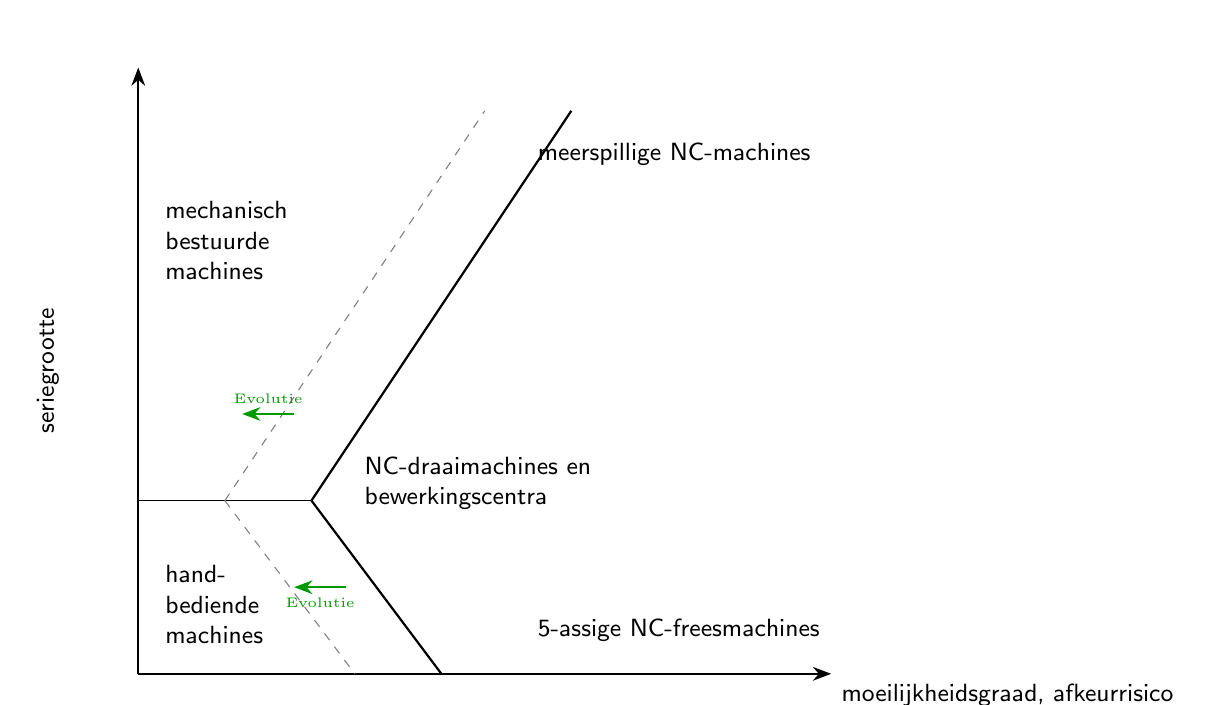
\begin{tikzpicture}[>=Stealth, font=\sffamily\small, scale=1.1]
		% Assen tekenen
		\draw[thick, ->] (0,0) -- (0,7) node[midway, left=25pt, rotate=90, anchor=south] {seriegrootte};
		\draw[thick, ->] (0,0) -- (8,0) node[anchor=north west] {moeilijkheidsgraad, afkeurrisico};

		% De horizontale scheidingslijn aan de linkerkant
		\draw (0, 2) -- (2, 2);

		% De gestreepte lijnen (starten vanaf het midden van de horizontale lijn) - Oude situatie
		\draw[dashed, gray] (1, 2) -- (4, 6.5);
		\draw[dashed, gray] (1, 2) -- (2.5, 0);

		% De doorgetrokken lijnen (starten vanaf het uiteinde van de horizontale lijn) - Nieuwe situatie
		\draw[thick] (2, 2) -- (5, 6.5);
		\draw[thick] (2, 2) -- (3.5, 0);

		% Tekst labels toevoegen
		% Linksboven
		\node[align=left, anchor=west] at (0.2, 5) {mechanisch\\bestuurde\\machines};
		% Rechtsboven
		\node[align=left, anchor=west] at (4.5, 6) {meerspillige NC-machines};
		% Linksonder
		\node[align=left, anchor=west] at (0.2, 0.8) {hand-\\bediende\\machines};
		% Midden rechts
		\node[align=left, anchor=west] at (2.5, 2.2) {NC-draaimachines en\\bewerkingscentra};
		% Rechtsonder
		\node[align=left, anchor=west] at (4.5, 0.5) {5-assige NC-freesmachines};
		% Legenda/Indicatie verschuiving (Arrows reversed: now pointing towards the boundaries to show expansion)
		\draw[<-, green!60!black, thick] (1.2, 3) -- (1.8, 3) node[midway, above, font=\tiny] {Evolutie};
		\draw[<-, green!60!black, thick] (1.8, 1) -- (2.4, 1) node[midway, below, font=\tiny] {Evolutie};
	\end{tikzpicture}
	\caption{K-grafiek: Toepassingsgebied van diverse productiesystemen in functie van seriegrootte en moeilijkheidsgraad. De verschuiving van de grenzen toont de groeiende inzetbaarheid van NC-technologie.}\label{fig:k_grafiek_user}
\end{figure}

\subsection{CAM}
CAD (Computer Aided Design) is het ontwerpen van modellen op de computer.
CAM (Computer Aided Manufacturing) is het omzetten van deze modellen naar bewerkingsprogramma's.
Vandaag de dag werken deze dingen hand in hand met de computer.
Je ontwerpt een model in CAD and dan kun je dit model importeren in CAM-software.
In deze CAM-software kun je dan bewerkingen definiëren zoals frezen, boren, zagen, enz.
De CAM-software genereert dan CL-data, dit is coördinaatcode (geen G-code), daarna wordt er voor de specifieke machine G-code gegenereerd.
\begin{figure}[ht]
	\centering
	\includegraphics[width=0.3\textwidth]{WorkflowCADCAM.png}
	\caption{Workflow van CAD naar CAM: proces van het ontwerpen van modellen in CAD-software en het genereren van bewerkingsprogramma's in CAM-software voor productie}
	\label{fig:WorkflowCADCAM.png}
\end{figure}
\FloatBarrier

In de moderne industrie wordt dit allemaal toegepast.
Je maakt je CAD, je importeert in CAM, je genereert G-code en je stuurt dit naar de machine via een netwerk. NC-machines op het netwerk zetten kan ook helpen voor monitoring en onderhoud. Je kunt stappen via de computer volgen.

\begin{warningbox}[title=EXAMEN CHECKLIST: MACHINES \& AUTOMATISERING]
    \begin{itemize}
        \item \textbf{Tijden}: Ken het verschil tussen hoofdtijd en neventijd en de invloed van seriegrootte op de totale kosten.
        \item \textbf{Automatisering}: Onderscheid starre (mechanische) en flexibele (NC/CNC) automatisering.
        \item \textbf{G-code}: Begrijp de structuur van een G-programma (G0, G1, M-functies).
        \item \textbf{K-grafiek}: Leg uit hoe de inzetbaarheid van NC-machines groeit door lagere instelkosten en hogere flexibiliteit.
        \item \textbf{CAD/CAM}: Begrijp de workflow van digitaal ontwerp naar machine-instructies via CL-data en post-processing.
    \end{itemize}
\end{warningbox}

\chapter{Productie werkvoorbereiding}
\section{Inleiding}
Werkvoorbereiding is het proces waarbij je alle stappen plant en organiseert die nodig zijn om een product te maken.

De centrale vraag bij werkvoorbereiding is: \textbf{Hoe gaan we dit product maken met de beschikbare middelen?}

Niet elk bedrijf heeft alle mogelijke productieprocessen in huis. Je moet dus keuzes maken op basis van wat er beschikbaar is (machinepark, gereedschappen) of beslissen wat eventueel uitbesteed moet worden.

Het totale voortbrengingsproces doorloopt doorgaans de volgende stadia:
\begin{enumerate}
	\item \textbf{Materiaalbereiding}: De winning en basisverwerking van grondstoffen tot halffabricaten.
	\item \textbf{Primaire vormgeving (Oervormen)}: Het creëren van een eerste ruwe vorm uit vormloos materiaal. Een typisch voorbeeld is gieten, wat vaak rendabel is bij grotere series.
	\item \textbf{Secundaire vormgeving (Bewerken)}: De verdere afwerking van de ruwe vorm naar een nauwkeurig product. Dit omvat technieken zoals verspanen (frezen, draaien), lassen of buigen.
	\item \textbf{Materiaalbehandeling}: Het aanpassen van de intrinsieke materiaaleigenschappen, bijvoorbeeld de hardheid verhogen door een warmtebehandeling.
	\item \textbf{Oppervlaktebehandeling}: Het wijzigen van de eigenschappen van het oppervlak, bijvoorbeeld voor corrosiebescherming of esthetiek (coaten, anodiseren, lakken).
	\item \textbf{Montage of assemblage}: Het samenvoegen van de verschillende geproduceerde onderdelen tot één werkend eindproduct.
\end{enumerate}

\textbf{Macrowerkmethode}: Je gaat ruim kijken hoe je het product gaat maken. Welke machines en processen ga je gebruiken.
Welke verspanningen en afnames zijn nodig.

\textbf{Microwerkmethode}: Hier ga je duiken in de details zoals wat is de voeding die ik moet gebruiken. Welke snijsnelheid, welke gereedschappen, welke koelvloeistof, enz.

\section{Het bewerkingsplan. De macrowerkmethode}
Het bewerkingsplan is relevant voor de macrowerkmethode.
Hier ga je kijken naar de verschillende processen die je kunt gebruiken om je product te maken.
Je bewerkingsplan hangt af van heel wat factoren:
\begin{itemize}
	\item \textbf{Seriegrootte en totaalserie}: Hoeveel producten ga je maken. Bij grote series kun je investeren in duurdere machines en processen.
	\item \textbf{Werkstukmateriaal}: Je hebt zacht maar ook harde materialen. Soms limiteert dit je keuze van proces.
	\item \textbf{Toleranties}: Hoe nauwkeurig moet het product zijn.
	\item \textbf{Afmetingen en vorm}: De geometrie van het product kan bepaalde processen uitsluiten of sommige processen vereisen.
	\item \textbf{Beschikbare machines en middelen}: Je moet kijken wat er beschikbaar is in de fabriek en het personeel dat je hebt.
	\item \textbf{Levertijd}: Hoe snel moet het product klaar zijn. Sommige processen zijn sneller dan andere.
\end{itemize}

Je moet duidelijk weten wat mogelijk is en wat de beperkingen zijn. De kosten van deze processen moeten ook in rekening worden gebracht. Bij het opstellen van een bewerkingsplan is er vaak niet één enkel correct antwoord; verschillende keuzes kunnen verdedigbaar zijn, zolang ze goed gemotiveerd worden op basis van factoren zoals de vereiste accuraatheid, de kostprijs, de productiesnelheid en de serie-grootte.

\begin{examenbox}
	Motiveer je keuzes voor een specifiek proces altijd aan de hand van technische en economische criteria.
\end{examenbox}

\subsection{Positionering}

\begin{conceptbox}[title=3-2-1 Methode]
    Om een werkstuk eenduidig vast te leggen in de ruimte (alle 6 vrijheidsgraden beperken), gebruiken we de 3-2-1 regel:
    \begin{itemize}
        \item \textbf{3 punten} bepalen het hoofdvlak (beperkt 3 vrijheidsgraden).
        \item \textbf{2 punten} bepalen de oriëntatie (beperkt 2 vrijheidsgraden).
        \item \textbf{1 punt} bepaalt de positie (beperkt de laatste vrijheidsgraad).
    \end{itemize}
\end{conceptbox}

Bij het positioneren wordt het werkstuk nauwkeurig in de machine geplaatst ten opzichte van een gekozen nulpunt of referentievlak. Het doel is om het werkstuk eenduidig vast te leggen in de ruimte, zodat de machine exact weet waar de bewerkingen moeten plaatsvinden. Hiervoor moet men vaak eerst een referentievlak bepalen door het werkstuk op te meten.

Een fundamenteel principe hierbij is de \textbf{3-2-1 methode}, die wordt gebruikt om de vrijheidsgraden van het werkstuk te minimaliseren en het eenduidig te positioneren:
\begin{itemize}
	\item \textbf{3 punten} bepalen het primaire vlak (meestal het grootste steunvlak).
	\item \textbf{2 punten} bepalen de oriëntatie ten opzichte van een tweede, loodrecht vlak.
	\item \textbf{1 punt} bepaalt de definitieve positie ten opzichte van het derde vlak.
\end{itemize}
Op deze manier ligt de positie van het werkstuk volledig vast zonder dat het systeem overbepaald is.

\autofig[0.45\textwidth]{positioneren.png}{Positioneren van het werkstuk volgens het 3-2-1 principe: bepalen van de juiste oriëntatie en referentiepunten.}

\subsection{Klemmen}
Nadat het werkstuk correct is gepositioneerd, moet het stevig worden vastgezet (opgespannen). Het doel van klemmen is om alle resterende vrijheidsgraden weg te nemen en te garanderen dat het werkstuk niet verschuift of trilt onder invloed van de proceskrachten (zoals de snijkrachten van de frees of beitel). De klemming gebeurt meestal door middel van wrijvingskrachten of directe mechanische klemkracht.

Er zijn verschillende methoden en hulpmiddelen beschikbaar voor het opspannen:
\begin{itemize}
	\item \textbf{Bankschroef}: De meest gebruikte methode voor prismatische werkstukken.
	\item \textbf{T-bouten en klemplaten}: Hiermee kan het werkstuk direct op de machinetafel worden gemonteerd.
	\item \textbf{Magneetklemmen}: Vooral geschikt voor vlakke, ferromagnetische materialen (vaak bij slijpen).
	\item \textbf{Vacuümklemmen}: Ideaal voor het opspannen van dunne platen of niet-magnetische materialen.
\end{itemize}

\autofig[0.3\textwidth]{image82.png}{Klemmen van het werkstuk: diverse methoden om het werkstuk stabiel te fixeren tijdens de bewerking.}

\subsection{Ondersteuning}
Naast positionering en klemmen is ondersteuning cruciaal, zeker bij complexe of minder stijve werkstukken. Ondersteuning dient niet enkel om het eigen gewicht van het stuk te dragen, maar vooral om vervorming door de grote snijkrachten tegen te gaan. 

Zonder de juiste ondersteuning kan het werkstuk gaan doorbuigen of kunnen er trillingen (\textit{chatter}) ontstaan. Dit leidt tot een slecht oppervlaktekwaliteit en afwijkingen in de maatvoering. In de figuur hieronder is te zien hoe ondersteuning helpt om deze buiging te voorkomen.

\autofig[0.3\textwidth]{voorkomenbuiging.png}{Ondersteuning van het werkstuk: het gebruik van steunpunten om doorbuiging en trillingen tijdens de bewerking te minimaliseren.}

\subsection{Universeel en product specifiek opspansysteem}
Een belangrijke keuze in het bewerkingsplan is het type opspansysteem.
Afhankelijk van de seriegrootte en de diversiteit van de producten, kies je tussen een universeel of een productspecifiek systeem.

\begin{itemize}
	\item \textbf{Productspecifiek opspansysteem}: Bij grote series is het rendabel om een opspanning op maat te maken (een mal). Het ontwerpen en maken kost tijd en geld, maar het wisselen van werkstukken gaat daarna zeer snel en nauwkeurig.
	\item \textbf{Universeel opspansysteem}: Bij kleine series of enkelstuks is flexibiliteit belangrijker. Universele systemen (zoals modulaire opspantafels) werken als een bouwdoos met gatenpatronen, klemmen en steunen. Hiermee kun je snel schakelen tussen verschillende producten zonder hoge investeringskosten per product.
\end{itemize}

\autofig[0.3\textwidth]{universeeltegenspecifiek.png}{Universeel klemmen versus productspecifiek klemmen: flexibele modulaire systemen versus op maat gemaakte mallen.}

\subsection{Nauwkeurigheid en ruwheid}
Het bewerkingsplan wordt sterk bepaald door de vereiste toleranties en oppervlaktekwaliteit. Niet elk proces kan elke nauwkeurigheid halen.

\begin{figure}[ht]
	\centering
	\includegraphics[width=0.45\textwidth]{tolerantie.png}
	\includegraphics[width=0.45\textwidth]{Ruwheid.png}
	\caption{Toleranties en ruwheid van verschillende bewerkingsprocessen: overzicht van haalbare maattoleranties en oppervlaktekwaliteiten.}
\end{figure}

\section{Microvoorbereiden en bewerkingsstappen}
Bij de microwerkmethode kijk je naar de specifieke stappen binnen één bewerking. Hierbij maak je onderscheid tussen ruwen en finiseren.

\begin{conceptbox}
	\textbf{Ruwe bewerking (Roughing):} Het doel is om zo snel mogelijk materiaal te verwijderen (hoge \textit{Material Removal Rate}). 
	Hierbij gebruik je grote snededieptes en voedingen. De oppervlaktekwaliteit en maattolerantie zijn hier nog van minder belang.
\end{conceptbox}

\begin{conceptbox}
	\textbf{Finiseren (Finishing):} Na het ruwen volgt de nabewerking om de definitieve maatvoering en oppervlaktekwaliteit te bereiken. 
	Hier werk je met kleinere afnames en fijnere voedingen.
\end{conceptbox}

Vaak zijn er meerdere stappen nodig (bijvoorbeeld: grof ruwen, half-finiseren, finiseren) om de gewenste nauwkeurigheid te halen, zeker als er veel materiaal moet worden weggenomen waardoor interne spanningen kunnen vrijkomen.

\autofig[1\textwidth]{image83.png}{Bewerkingstoegift: Eerst ruwen met grote afnames, gevolgd door finiseren met kleine afnames voor het eindresultaat.}

\subsection{Computerondersteunde werkvoorbereiding (CAPP)}
Computer Aided Process Planning (CAPP) automatiseert het maken van werkvoorbereidingen. We onderscheiden twee hoofdmethoden:

\begin{itemize}
	\item \textbf{Variant methode (Retrieval type)}: Het systeem zoekt in een database naar een bestaand bewerkingsplan van een vergelijkbaar product (een "variant") en past dit aan voor het nieuwe product. Dit is gebaseerd op Groepentechnologie (GT).
	\item \textbf{Generatieve methode}: Het systeem genereert een volledig nieuw bewerkingsplan "from scratch" op basis van het 3D-model, technologieregels, machinespecificaties en logaritmen, zonder terug te grijpen naar oude plannen.
\end{itemize}

\begin{examenbox}
	\textbf{Belangrijke aandachtspunten voor Microvoorbereiding:}
	\begin{itemize}
		\item \textbf{Minimaliseer wissels}: Vermijd onnodige gereedschapswissels en zeker heropspanningen. Elke nieuwe opspanning introduceert onnauwkeurigheden.
		\item \textbf{Referentievlakken}: Kies je referentievlakken slim. Vorm- en plaatstoleranties hangen af van hoe je het stuk vasthoudt.
		\item \textbf{Volgorde}: Bewerk nauwkeurige vlakken (bv. IT7/IT8) pas aan het einde. 
		      Halffabricaten bevatten vaak interne spanningen die vrijkomen bij het wegnemen van materiaal ("werking" van het materiaal), wat tot vervorming kan leiden als je te vroeg finiseert.
	\end{itemize}
\end{examenbox}

\begin{examenbox}
	Op het examen moet je voor producten van verschillende complexiteit (zie figuur \ref{fig:lossestukken}) een bewerkingsplan kunnen opstellen en motiveren aan de hand van de gekende technieken.
\end{examenbox}

	\begin{center}
		\includegraphics[width=0.5\textwidth]{image84.png}
		\captionof{figure}{Producten die verschillen in complexiteit.}
		\label{fig:lossestukken}
	\end{center}

Om een goed plan op te stellen, moet je de eigenschappen (voordelen, nadelen en nauwkeurigheid) kennen van de volgende technieken:
\begin{itemize}
    \item \textbf{Gieten}: Zandgieten, verloren wasmodel, permanent gieten (spuitgieten).
    \item \textbf{Verspanen}: Frezen, draaien en slijpen.
    \item \textbf{Speciale bewerkingen}: Vonkeroderen (EDM), laserbewerking en waterstraalsnijden.
    \item \textbf{Vervormen \& Scheiden}: Ponsen, snijden en kappen.
    \item \textbf{Behandelingen}: Harden en andere warmtebehandelingen.
\end{itemize}

\subsection{Flowchart: Het Werkvoorbereidingsproces}
Onderstaande flowchart geeft een overzicht van de stappen in de werkvoorbereiding, van ontwerp tot productie, met onderscheid tussen de macro- en microfase.

\begin{figure}[ht]
	\centering
	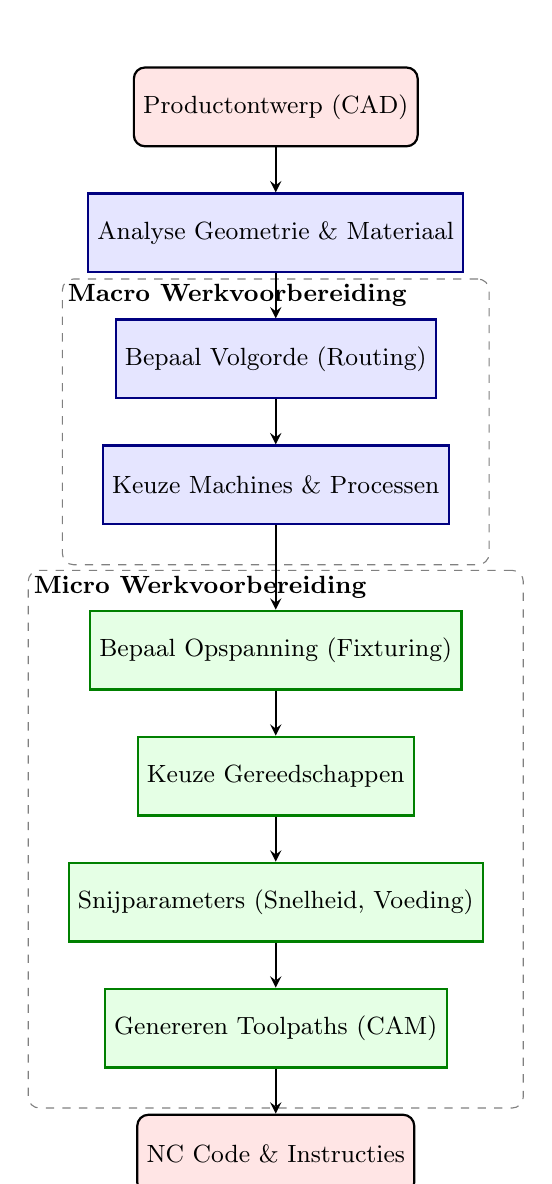
\begin{tikzpicture}[
			node distance=1.6cm,
			every node/.style={font=\small},
			startstop/.style={rectangle, rounded corners, minimum width=3cm, minimum height=1cm, text centered, draw=black, fill=red!10, thick},
			macro/.style={rectangle, minimum width=3.5cm, minimum height=1cm, text centered, draw=blue!50!black, fill=blue!10, thick},
			micro/.style={rectangle, minimum width=3.5cm, minimum height=1cm, text centered, draw=green!50!black, fill=green!10, thick},
			decision/.style={diamond, aspect=2, minimum width=3cm, minimum height=0.8cm, text centered, draw=black, fill=orange!10, thick},
			arrow/.style={thick,->,>=stealth},
			groupbox/.style={draw=gray, dashed, inner sep=0.5cm, rounded corners, label={[anchor=north west, inner sep=2pt]north west:\textbf{#1}}}
		]

		% Nodes
		\node (start) [startstop] {Productontwerp (CAD)};
		\node (analysis) [macro, below of=start] {Analyse Geometrie \& Materiaal};
        
		% Macro Group
		\node (routing) [macro, below of=analysis] {Bepaal Volgorde (Routing)};
		\node (machine) [macro, below of=routing] {Keuze Machines \& Processen};
        
		% Micro Group
		\node (fix) [micro, below of=machine, yshift=-0.5cm] {Bepaal Opspanning (Fixturing)};
		\node (tools) [micro, below of=fix] {Keuze Gereedschappen};
		\node (params) [micro, below of=tools] {Snijparameters (Snelheid, Voeding)};
		\node (cam) [micro, below of=params] {Genereren Toolpaths (CAM)};
        
		\node (end) [startstop, below of=cam] {NC Code \& Instructies};

		% Annotations for Macro/Micro
		\node[fit=(routing)(machine), groupbox={Macro Werkvoorbereiding}] (macrogroup) {};
		\node[fit=(fix)(tools)(params)(cam), groupbox={Micro Werkvoorbereiding}] (microgroup) {};

		% Connections
		\draw [arrow] (start) -- (analysis);
		\draw [arrow] (analysis) -- (routing);
		\draw [arrow] (routing) -- (machine);
		\draw [arrow] (machine) -- (fix);
		\draw [arrow] (fix) -- (tools);
		\draw [arrow] (tools) -- (params);
		\draw [arrow] (params) -- (cam);
		\draw [arrow] (cam) -- (end);

	\end{tikzpicture}
	\caption{Flowchart van de werkvoorbereiding: van Macro-beslissingen (procesniveau) naar Micro-beslissingen (operationeel niveau).}\label{fig:werkvoorbereiding_flowchart_detail}
\end{figure}
\FloatBarrier

\begin{warningbox}[title=EXAMEN CHECKLIST: WERKVOORBEREIDING]
    \begin{itemize}
        \item \textbf{Macro vs. Micro}: Onderscheid beslissingen op procesniveau (routing, machinekeuze) en operationeel niveau (opspanning, tools, parameters).
        \item \textbf{3-2-1 methode}: Leg uit hoe je een werkstuk eenduidig positioneert door vrijheidsgraden te beperken zonder overbepaaldheid.
        \item \textbf{Klemmen}: Begrijp het doel (tegen gaan proceskrachten) en ken de hulpmiddelen (bankschroef, vacuüm).
        \item \textbf{CAPP}: Onderscheid de variant methode (GT-gebaseerd) en de generatieve methode (vanaf nul).
        \item \textbf{Referentievlakken}: Begrijp dat alle toleranties afhangen van het gekozen referentievlak en heropspanningen vermeden moeten worden.
    \end{itemize}
\end{warningbox}

\chapter{Productiegericht ontwerpen}
\section{Inleiding}
Productiegericht ontwerpen (Design for Manufacturing, DFM) is het proces waarbij het productontwerp optimaal wordt afgestemd op de beschikbare productieprocessen en fabricagetechnieken. Het doel is om de totale kosten te minimaliseren en tegelijkertijd de kwaliteit en maakbaarheid te verhogen.

Bij een integraal ontwerp kijkt men niet enkel naar de productie, maar ook naar:
\begin{itemize}
	\item \textbf{Design for Assembly (DFA)}: Het ontwerp optimaliseren voor een snelle en foutloze montage.
	\item \textbf{Design for Logistics}: Optimalisatie van verpakking en materiaalstromen.
	\item \textbf{Design for Recycling/Maintenance}: Rekening houden met de volledige levenscyclus, inclusief onderhoud en demontage voor recyclage (Demanufacturing).
\end{itemize}

\autofig[0.45\textwidth]{gemaaktEnVastgelegdeKosten.png}{Gerealiseerde versus vastgelegde kosten: Hoewel de ontwerpfase zelf relatief weinig kost, wordt hier het grootste deel van de uiteindelijke productiekosten vastgelegd.}

De ontwerper heeft dus een enorme impact op de uiteindelijke kostprijs door rekening te houden met de functie, maakbaarheid, onderhoudbaarheid en duurzaamheid van het product.

\section{Designen voor verspaanbewerkingen}
In de maakwereld is perfectie onmogelijk. Een ontwerper moet begrijpen dat gereedschappen hun beperkingen hebben. Zo is het onmogelijk om een perfecte binnenhoek te frezen met een scherpe rand; de radius van de frees bepaalt altijd de kleinst mogelijke afronding in de hoek.

\autofig[0.4\textwidth]{imperfectiefrezen.png}{Beperkingen bij frezen: De radius van het gereedschap maakt het onmogelijk om perfect scherpe binnenhoeken te creëren.}

\section{Designen voor toeslagen}
Wanneer een product een nabewerking vereist (zoals slijpen na het harden), moet de ontwerper zorgen dat de betreffende oppervlakken goed toegankelijk zijn voor de bewerkingstools. Ook moet er voldoende 'toegift' (extra materiaal) voorzien worden, rekening houdend met de toleranties van de voorgaande bewerkingen.

\autofig[0.6\textwidth]{designenvoortoeslagen.png}{Designen voor toeslagen: Het voorzien van voldoende bewerkingstoegift en toegankelijkheid voor gereedschappen.}

\section{Designen voor matrijzen}
Bij gieten of spuitgieten moet men rekening houden met de lossing (vrijloophoeken), een gelijkmatige wanddikte om slink te voorkomen, en het vermijden van ondersnijdingen die de matrijs complex en duur maken.

\section{Algemene regels bij Design for Manufacturing (DFM)}
\begin{itemize}
	\item \textbf{Vermijd scherpe hoeken}: Deze veroorzaken spanningsconcentraties en verhogen het risico op breuk of scheurvorming. Gebruik afrondingen (fillets).

	\begin{figure}[ht]
		\centering
		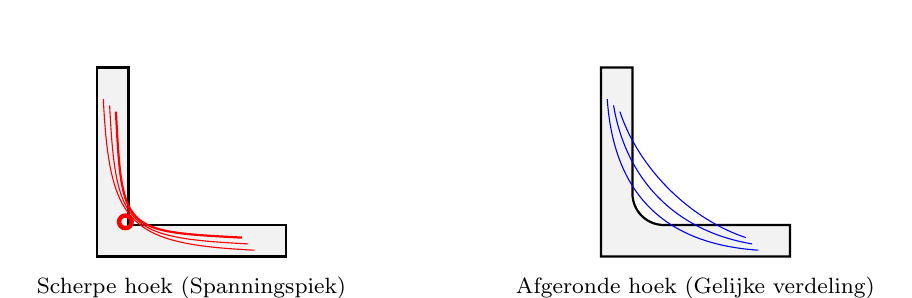
\begin{tikzpicture}[scale=0.8]
			% Sharp corner
			\begin{scope}[xshift=-4cm]
				\draw[thick, fill=gray!10] (0,3) -- (0,0) -- (3,0) -- (3,0.5) -- (0.5,0.5) -- (0.5,3) -- cycle;
				% Stress lines (concentrated at corner)
				\draw[red, thin] (0.1, 2.5) .. controls (0.2, 0.5) and (0.5, 0.2) .. (2.5, 0.1);
				\draw[red, thin] (0.2, 2.4) .. controls (0.3, 0.45) and (0.45, 0.3) .. (2.4, 0.2);
				\draw[red, thick] (0.3, 2.3) .. controls (0.4, 0.4) and (0.4, 0.4) .. (2.3, 0.3);
				\draw[red, ultra thick] (0.45, 0.55) circle (0.1); % Point of concentration
				\node at (1.5, -0.5) {\footnotesize Scherpe hoek (Spanningspiek)};
			\end{scope}

			% Rounded corner
			\begin{scope}[xshift=4cm]
				\draw[thick, fill=gray!10] (0,3) -- (0,0) -- (3,0) -- (3,0.5) -- (1,0.5) arc(270:180:0.5) -- (0.5,1) -- (0.5,3) -- cycle;
				% Stress lines (distributed)
				\draw[blue, thin] (0.1, 2.5) .. controls (0.2, 1) and (1, 0.2) .. (2.5, 0.1);
				\draw[blue, thin] (0.2, 2.4) .. controls (0.4, 1.2) and (1.2, 0.4) .. (2.4, 0.2);
				\draw[blue, thin] (0.3, 2.3) .. controls (0.6, 1.4) and (1.4, 0.6) .. (2.3, 0.3);
				\node at (1.5, -0.5) {\footnotesize Afgeronde hoek (Gelijke verdeling)};
			\end{scope}
		\end{tikzpicture}
		\caption{Visualisatie van spanningsconcentraties: Een scherpe hoek veroorzaakt een ophoping van spanningslijnen. Een afronding verdeelt de krachten gelijkmatiger.}\label{fig:spanningsconcentratie}
	\end{figure}

	\item \textbf{Minimaliseer het aantal onderdelen}: Hoe minder onderdelen, hoe lager de montagekosten en het risico op fouten.
	\item \textbf{Standaardiseer onderdelen}: Gebruik zoveel mogelijk standaardcomponenten (bouten, lagers) om voorraadkosten te drukken.
	\item \textbf{Modulair ontwerp}: Bouw producten op uit herbruikbare modules die in verschillende configuraties toegepast kunnen worden.
	\item \textbf{Multifunctionele onderdelen}: Probeer meerdere functies te integreren in één onderdeel.
	\item \textbf{Kies realistische toleranties}: Te nauwe toleranties verhogen de kostprijs exponentieel zonder altijd functionele meerwaarde te bieden.
	\item \textbf{Kies goed bewerkbare materialen}: Stem de materiaalkeuze af op de gewenste bewerkingstechniek.
\end{itemize}

\begin{figure}[ht]
	\centering
	\includegraphics[width=0.3\textwidth]{regelsDFM.png}
	\caption{Overzicht van DFM-regels: Samenvatting van de belangrijkste richtlijnen voor productiegericht ontwerpen.}
	\label{fig:DFMregels.png}
\end{figure}

\begin{conceptbox}
	\textbf{Design for Manufacturing (DFM) VS Manufacturing for Design (MFD)}:
	\newline
	In dit hoofdstuk hebben we allemaal beperkingen gelegd op het ontwerp ter bevordering van de productie. Dit is DFM.
	\newline
	MFD is het omgekeerde. Hier ga je kijken naar de productieprocessen en hoe je deze kunt aanpassen om beter aan de ontwerpvereisten te voldoen. 
	MFD is duurder maar kan wel technologieën voortduwen en nieuwe productietechnologie mogelijk maken.
	3D printen is ontstaan uit de vraag om makkelijker specifieke eenmalige producten te maken.
\end{conceptbox}

\begin{warningbox}[title=EXAMEN CHECKLIST: PRODUCTIEGERICHT ONTWERPEN]
    \begin{itemize}
        \item \textbf{DFM vs. DFA}: Begrijp het verschil tussen ontwerpen voor maakbaarheid en ontwerpen voor assemblage.
        \item \textbf{Scherpe hoeken}: Leg uit waarom afrondingen (fillets) spanningsconcentraties voorkomen.
        \item \textbf{Standaardisatie}: Weet dat standaardonderdelen en modules de kosten en complexiteit verlagen.
        \item \textbf{Impact}: Onthoud dat de ontwerper tot 70-80\% van de uiteindelijke productiekosten vastlegt.
        \item \textbf{Toleranties}: Begrijp dat over-specificeren van toleranties de prijs onnodig opdrijft.
    \end{itemize}
\end{warningbox}

\chapter{Examentips}

Als je een vraag krijgt, wees dan duidelijk in je antwoord.

Schrijf niet enorm grote paragrafen. Een tekening met een korte uitleg is vaak beter.

Bekijk de laatste video op toledo waar hij over een voorbeeldexamen gaat.



\chapter{Slotwoord}

Ik heb 4-dagen van de blok gestoken in het maken van deze samenvatting.

Ik hoop dat jullie er veel aan hebben gehad en dat het jullie helpt bij het studeren voor

de examens.



\textbf{Ruben out}



\newpage

\chapter*{Succes!}

\vfill

\begin{center}

	\itshape\Huge

	Veel succes met de examens!

	\par\vspace{1cm}

	\normalfont\Large

	--- Ruben Ryckaert

\end{center}



\vspace{3cm}



\begin{quote}

	\centering

	\itshape\Large

	``Yesterday is history, tomorrow is a mystery, but today is a gift. That is why it is called the present.''

	\par\vspace{0.5cm}

	\textup{--- Oogway}

\end{quote}

\vfill



\end{document}